\chapter{Review of CADe and CADx for CaP}\label{chap:3}
% the code below specifies where the figures are stored
\ifpdf
    \graphicspath{{3_review/figures/}}
\else
    \graphicspath{{3_review/figures/}}
\fi


As previously mentioned in the introduction (see \acs{sec}~\ref{sec:intro:cad}), \acp{cad} are developed to advise and backup radiologists in their tasks of \ac{cap} detection and diagnosis, but not to provide fully automatic decisions \cite{Giger2008}.
\acp{cad} can be divided into two different sub-groups either as \ac{cade}, with the purpose to highlight probable lesions in \ac{mri} images, or \ac{cadx}, which focuses on differentiating malignant from non-malignant tumours \cite{Giger2008}.
Moreover, an intuitive approach, motivated by developing a framework combining detection-diagnosis, is to mix both \ac{cade} and \ac{cadx} by using the output of the former mentioned as a input of the latter named.
Although the outcomes of these two systems should differ, the framework of both \ac{cad} systems is similar.
A general \ac{cad} work-flow is presented n \acs{fig}~\ref{fig:wkfcad}. 
%The \ac{cad} work-flow is presented in \acs{fig}~\ref{fig:wkfcad}.

\ac{mri} modalities mentioned in \acs{sec}~\ref{subsubsec:mrimrsi} are used as inputs of \ac{cad} for \ac{cap}.
These images acquired from the different modalities show a large variability between patients: the prostate organ can be located at different positions in images (e.g., patient motion, variation of acquisition plan), and the \ac{si} can be corrupted with noise or artefacts during the acquisition process (eg., magnetic field inhomogeneity, use of endorectal coil).
%It can be noted that \ac{adc} map is not considered as an input since it is a feature derived from the \ac{dw} \ac{mri} images.
To address these issues, the first stage of \ac{cad} is to pre-process multiparametric \ac{mri} images to reduce noise, remove artefacts and standardize the \ac{si}.
At most of the later processes will be only focused on the prostate, it is necessary to segment the prostate in each \ac{mri}-modality to define it as a \acs{roi}.
However, data may suffer from misalignment due to patient motions or different acquisition parameters.
Therefore, a registration step is usually performed so that all the previously segmented \ac{mri} images will be in the same reference frame.
Registration and segmentation can be swapped depending on the strategy chosen.

Some studies do not fully apply the methodology depicted in \acs{fig}.~\ref{fig:wkfcad}.
Details about those can be found in \acs{tab}~\ref{tab:sumpap}.
Some studies proposed methods in which inputs are the \ac{mri} raw data inorder to demostrate the robustness of their approaches to noise or artefacts.
In some cases, prostate segmentation is performed manually as well as registration.
It is also sometimes assumed that no patient motions occur during the acquisition procedure, removing the need of registering the multiparametric \ac{mri} images.

Once the data are regularized, it becomes possible to extract features and classify the data to obtain either the location of possible lesions (\ac{cade}) or/and the malignancy nature of these lesions (\ac{cadx}).

In \iac{cade} framework, \textit{possible lesions will be segmented automatically} and further used as input of \ac{cadx}.
Nevertheless, some works also used a fusion \ac{cade}-\ac{cadx} framework in which a voxel-based features are directly used, allowing to obtain the location of the malignant lesions as results.
On the other hand, manual lesions segmentation are not considered to be part of \ac{cade}.
The output of the \ac{cade} is used as input of the \ac{cadx}.

\Ac{cadx} is composed of the processes allowing to \textit{distinguish malignant from non-malignant tumours}.
Here, \ac{cap} malignancy is defined using the grade of the GS determined after post biopsy or prostatecomy.
As presented in \ac{fig}.~\ref{fig:wkfcad}, \ac{cadx} is usually composed of the three common steps used in classification framework: (i) features detection, (ii) feature extraction/selection and (iii) feature classification.


%% We divided \ac{cadx} into three different stages. First, salient features are extracted, in an pixel-based or region-based manner, from \ac{mri} images to characterize the lesion. Of course, more discriminative features will be associated with a robust and accurate likelihood cancer map. Frequently, the number of features extracted can be large resulting in redundant or insufficient discriminative features which will negatively affect the performances of the further classification. Therefore, a step consists of selecting the best features or/and reducing the number of dimensions is commonly used. Then, this modified feature vector is finally classified using different pattern recognition approaches.

%% As pointed out in the introduction, performance of \ac{cap} detection and diagnosis are affected by observer interpretation and limitations \cite{Giger2008,Hambrock2013}. \ac{cad} offers a possible solution in order to reduce this variability. As mentioned in the introduction, the effects of \ac{cad} on the observer performance has been studied \cite{Hambrock2013}, with results showing that \acp{cad} benefit to less-experienced radiologist to perform similarly as experienced radiologist in their tasks \cite{Hambrock2013}. 


%\section{Literature classification}\label{sec:chp3:Literature-classification}

This chapter is organized using the methodology presented in \acs{fig}.~\ref{fig:wkfcad}.
Methods embedded in the image regularization framework are presented initially to subsequently focus on the image classification framework, being divided into \ac{cade} and \ac{cadx}.
Finally presenting the results and the discussion driven from the state-of-the-art.
%before to focus on the image classification framework, the later being divided into \ac{cade} and \ac{cadx}. 
\Acl{tab}~\ref{tab:sumpap} summarizes the fourty-two different \ac{cad} studies reviewed in section.
The first set of information reported is linked to the data acquisition such as the number of patients included in the study, the modalities acquired as well as the strength of the field of the scanner used.
Subsequently, information about the prostate zones considered in the \ac{cad} analysis (\ac{pz} or \ac{cg}) are reported since that detecting \ac{cap} in the \ac{cg} is a more challenging problem and has received particular attention only in the recent publications.

%% Characteristics related to \ac{mri} acquisition as well as \ac{cad} strategies are reported.
%% Only methods used in \ac{cad} system are discussed.

\newgeometry{left=1cm,right=1cm,bottom=0.5cm,top=0.3cm}

\begin{table}
\centering
\caption{Overview of the different studies reviewed with their main characteristics. Acronyms: number (\#) - image regularization (Img. Reg.).}
\scriptsize
%\begin{adjustwidth}{-cm}{}
\begin{threeparttable}
\renewcommand{\arraystretch}{1}	
	\rowcolors{3}{black!5}{white}	
	\begin{tabular}{|>{\centering\arraybackslash}m{0.7cm}|>{\centering\arraybackslash}m{0.8cm}|>{\centering\arraybackslash}m{0.9cm}|>{\centering\arraybackslash}m{0.8cm}>{\centering\arraybackslash}m{0.8cm}>{\centering\arraybackslash}m{0.9cm}>{\centering\arraybackslash}m{0.8cm}|>{\centering\arraybackslash}m{0.6cm}>{\centering\arraybackslash}m{0.6cm}|>{\centering\arraybackslash}m{0.6cm}>{\centering\arraybackslash}m{0.6cm}|>{\centering\arraybackslash}m{0.6cm}>{\centering\arraybackslash}m{0.6cm}>{\centering\arraybackslash}m{0.65cm}|}\hline
	\hiderowcolors
	\multirow{2}{*}{Index} & \multirow{2}{*}{Study} & \# & \multicolumn{4}{c|}{\ac{mri}-modality} & \multicolumn{2}{c|}{Strength of field} & \multicolumn{2}{c|}{Studied zones} & \multicolumn{3}{c|}{\ac{cad} stages} \\ \cline{4-14}
	 & & patients & \ac{t2w} \ac{mri} & \ac{dce} \ac{mri} & \ac{dw} \ac{mri} & \ac{mrsi} & 1.5 T & 3.0 T & \ac{pz} & \ac{cg} & Img. Reg. & \ac{cade} & \ac{cadx} \\ \hline \hline
	 \showrowcolors 
	 	 $[1]$&\cite{Ampeliotis2007} & 25 & \cmark & \cmark & \xmark & \xmark & \cmark & \xmark & \cmark & \xmark & \mmark & \xmark & \cmark \\
	 	 $[2]$&\cite{Ampeliotis2008} & 25 & \cmark & \cmark & \xmark & \xmark & \cmark & \xmark & \cmark & \xmark & \mmark & \xmark & \cmark \\
	 	 $[3]$&\cite{Antic2013} & 53 & \cmark & \xmark & \cmark & \xmark & \cmark & \xmark & \cmark & \cmark & \xmark  & \xmark & \cmark \\
	 	 $[4]$&\cite{Artan2009} & 10 & \cmark & \cmark & \cmark & \xmark & \cmark & \xmark & \cmark & \xmark  & \xmark & \cmark & \cmark \\
	 	 $[5]$&\cite{Artan2010} & 21 & \cmark & \cmark & \cmark & \xmark & \cmark & \xmark & \cmark & \xmark & \mmark & \cmark & \cmark \\
	 	 $[6]$&\cite{Chan2003} & 15 & \cmark & \xmark & \cmark & \xmark & \cmark & \xmark & \cmark & \xmark & \xmark & \xmark & \cmark \\
	 	 $[7]$&\cite{Giannini2013} & 10 & \cmark & \cmark & \cmark & \xmark & \cmark & \xmark & \cmark & \xmark & \cmark & \cmark & \cmark \\
	 	 $[8]$&\cite{Kelm2007} & 24 & \xmark & \xmark & \xmark & \cmark & \cmark & \xmark & \cmark & \cmark & \mmark & \cmark & \cmark \\
	 	 $[9]$&\cite{Langer2009} & 25 & \cmark & \cmark & \cmark & \xmark & \cmark & \xmark & \cmark & \xmark & \mmark & \xmark & \cmark \\
	 	 $[10]$&\cite{Litjens2011} & 188 & \cmark & \cmark & \cmark & \xmark & \xmark & \cmark & \cmark & \xmark & \mmark & \cmark & \cmark \\
	 	 $[11]$&\cite{Litjens2012} & 288 & \cmark & \cmark & \cmark & \xmark & \xmark & \cmark & \cmark & \cmark & \mmark & \cmark & \cmark \\
	 	 $[12]$&\cite{Liu2009} & 11 & \cmark & \cmark & \cmark & \xmark & \cmark & \xmark & \cmark & \xmark & \mmark & \cmark & \cmark \\
	 	 $[13]$&\cite{Liu2013} & 54 & \cmark & \cmark & \cmark & \xmark & \xmark & \cmark & \cmark & \cmark & \mmark & \xmark & \cmark \\
	 	 $[14]$&\cite{Lopes2011} & 27 & \cmark & \xmark & \xmark & \xmark & \cmark & \xmark & \cmark & \xmark & \mmark & \cmark & \cmark \\
	 	 $[15]$&\cite{Lv2009} & 55 & \cmark & \xmark & \xmark & \xmark & \cmark & \xmark & \cmark & \xmark & \mmark & \xmark & \cmark \\
	 	 $[16]$&\cite{Matulewicz2013} & 18 & \xmark & \xmark & \xmark & \cmark & \xmark & \cmark & \cmark & \cmark & \xmark & \cmark & \cmark \\ 
	 	 $[17]$&\cite{Mazzetti2011} & 10 & \xmark & \cmark & \xmark & \xmark & \cmark & \xmark & \cmark & \xmark & \mmark & \cmark & \cmark \\
	 	 $[18]$&\cite{Niaf2011} & 23 & \cmark & \cmark & \cmark & \xmark & \cmark & \xmark & \cmark & \xmark & \mmark & \xmark & \cmark \\
	 	 $[19]$&\cite{Niaf2012} & 30 & \cmark & \cmark & \cmark & \xmark & \cmark & \xmark & \cmark & \xmark & \mmark & \xmark & \cmark \\
	 	 $[20]$&\cite{Ozer2009} & 20 & \cmark & \cmark & \cmark & \xmark & \cmark & \xmark & \cmark & \xmark & \mmark & \cmark & \cmark \\
	 	 $[21]$&\cite{Ozer2010} & 20 & \cmark & \cmark & \cmark & \xmark & \cmark & \xmark & \cmark & \xmark & \mmark & \cmark & \cmark \\
	 	 $[22]$&\cite{Parfait2012} & 22 & \xmark & \xmark & \xmark & \cmark & \xmark & \cmark & \cmark & \cmark & \mmark & \cmark & \cmark \\
	 	 $[23]$&\cite{Peng2013} & 48 & \cmark & \cmark & \cmark & \xmark & \xmark & \cmark & \cmark & \cmark & \xmark & \xmark & \cmark \\
	 	 $[24]$&\cite{Puech2009} & 100 & \xmark & \cmark & \xmark & \xmark & \cmark & \xmark & \cmark & \cmark & \xmark & \xmark & \cmark \\
	 	 $[25]$&\cite{Sung2011} & 42 & \xmark & \cmark & \xmark & \xmark & \xmark & \cmark & \cmark & \cmark & \xmark & \cmark & \cmark \\
	 	 $[26]$&\cite{Tiwari2007} & 14 & \xmark & \xmark & \xmark & \cmark & \cmark & \xmark & \cmark & \cmark & \mmark & \cmark & \cmark \\
	 	 $[27]$&\cite{Tiwari2008} & 18 & \xmark & \xmark & \xmark & \cmark & \cmark & \xmark & \cmark & \cmark & \mmark & \cmark & \cmark \\
	 	 $[28]$&\cite{Tiwari2009} & 18 & \xmark & \xmark & \xmark & \cmark & \cmark & \xmark & \cmark & \cmark & \mmark & \cmark & \cmark \\
	 	 $[29]$&\cite{Tiwari2009a} & 15 & \cmark & \xmark & \xmark & \cmark & \cmark & \xmark & \cmark & \cmark & \mmark & \cmark & \cmark \\
	 	 $[30]$&\cite{Tiwari2010} & 19 & \cmark & \xmark & \xmark & \cmark & \cmark & \xmark & \cmark & \cmark & \mmark & \cmark & \cmark \\
	 	 $[31]$&\cite{Tiwari2012} & 36 & \cmark & \xmark & \xmark & \cmark & \cmark & \xmark & \cmark & \cmark & \xmark & \cmark & \cmark \\
	 	 $[32]$&\cite{Tiwari2013} & 29 & \cmark & \xmark & \xmark & \cmark & \cmark & \xmark & \cmark & \cmark & \mmark & \cmark & \cmark \\
	 	 $[33]$&\cite{Viswanath2008} & 16 & \cmark & \xmark & \xmark & \cmark & \cmark & \xmark & \cmark & \cmark & \xmark & \cmark & \cmark \\
	 	 $[34]$&\cite{Viswanath2008a} & 6 & \cmark & \cmark & \xmark & \xmark & \xmark & \cmark & \cmark & \cmark & \mmark & \cmark & \cmark \\
	 	 $[35]$&\cite{Viswanath2009} & 6 & \cmark & \cmark & \xmark & \xmark & \xmark & \cmark & \cmark & \cmark & \cmark & \cmark & \cmark \\
	 	 $[36]$&\cite{Viswanath2011} & 12 & \cmark & \cmark & \cmark & \xmark & \xmark & \cmark & \cmark & \cmark & \mmark & \cmark & \cmark \\
	 	 $[37]$&\cite{Viswanath2012} & 22 & \cmark & \xmark & \xmark & \xmark & \xmark & \cmark & \cmark & \cmark & \cmark & \cmark & \cmark \\
	 	 $[38]$&\cite{Vos2008} & 29 & \cmark & \cmark & \xmark & \xmark & \cmark & \xmark & \cmark & \xmark & \mmark & \xmark & \cmark \\
	 	 $[39]$&\cite{Vos2008a} & 29 & \xmark & \cmark & \xmark & \xmark & \cmark & \xmark & \cmark & \xmark & \mmark & \xmark & \cmark \\
	 	 $[40]$&\cite{Vos2010} & 29 & \cmark & \cmark & \xmark & \xmark & \cmark & \xmark & \cmark & \xmark & \mmark & \xmark & \cmark \\
	 	 $[41]$&\cite{Vos2012} & NA & \cmark & \cmark & \cmark & \xmark & \xmark & \cmark & \cmark & \xmark & \mmark & \cmark & \cmark \\
	 	 \hline
	\end{tabular}
	\begin{tablenotes}
      \tiny
      \item Notes:
      \item {\xmark}: not used or not implemented.
      \item {\mmark}: partially implemented.
      \item {\cmark}: used or implemented.
    \end{tablenotes}
\end{threeparttable}
%\end{adjustwidth}
\label{tab:sumpap}
\end{table}

\restoregeometry

\section{Image regularization framework}\label{sec:chp3:img-reg}

This section provides a review of the methods used in \acp{cad} for \ac{cap} in order to \emph{regularize} the \ac{mpmri} images.
At first, we present the pre-processing methods in \acs{sec}\,\ref{subsec:chp3img-reg:prepro}, focusing mainly on the denoising and artefacts removal methods as well as standardization of \ac{si}.
\Acl{sec}~\ref{subsec:chp3:img-reg:seg} and \acs{sec}\,\ref{subsec:chp3:img-reg:reg} summarize the segmentation and registration methods, which are processes allowing the \ac{cad} to only operate on the prostate organ and ensuring that the \ac{mpmri} images are aligned in the same reference frame.

%We start with pre-processing methods, focusing mainly on the reduction of noise level and artefacts as well as standardization of \ac{si}, following by a segmentation and registration sections.

\subsubsection{Pre-processing}\label{subsubsec:chp3:lit-clas:img-reg:prepro}
Three different groups of pre-processing methods are commonly applied to images as initial stage in \ac{cad} for \ac{cap}.
These methods are explained for both \ac{mri} and \ac{mrsi} modalities, while a summary of the applied methods in \ac{cad} is presented in Table.~\ref{tab:summary-preproc}.

\setenumerate{listparindent=\parindent,itemsep=10px}
\setlist{noitemsep}
\begin{enumerate}[leftmargin=*]

\begin{figure}
\centering
	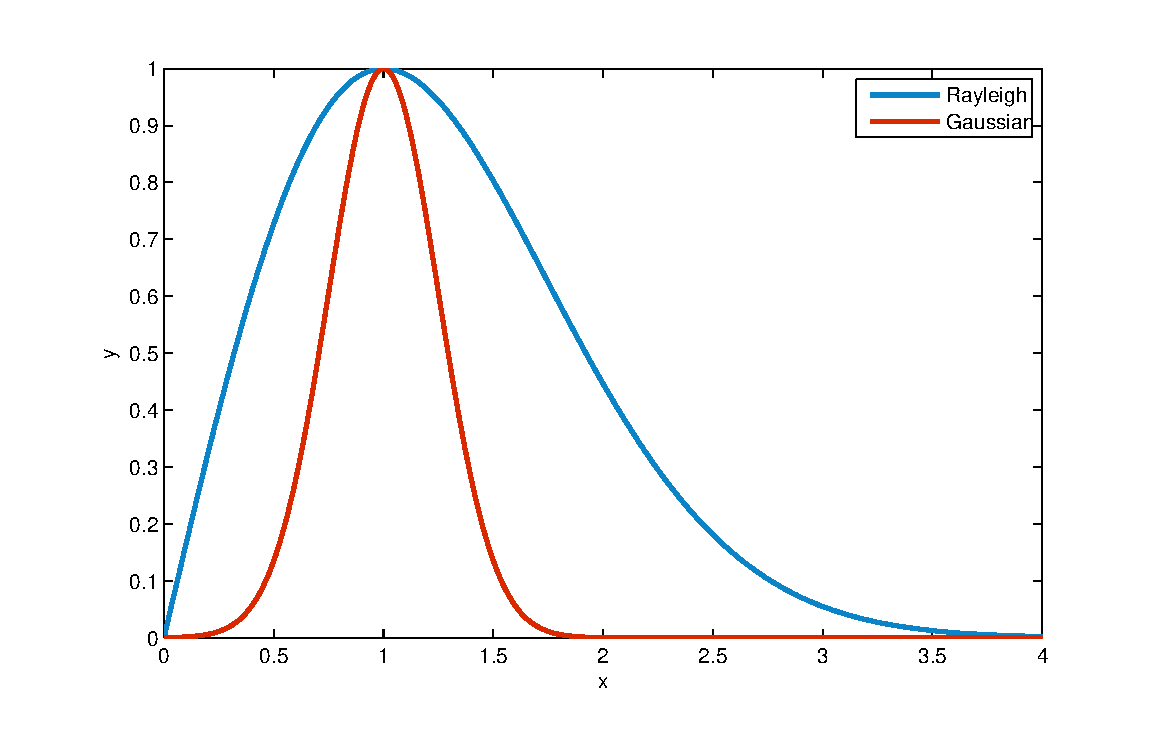
\includegraphics[width=0.7\linewidth]{3_review/figures/processing/pre-processing/noise/noisedistr.eps}
	\caption[Illustration of a Gaussian and Rayleigh distributions.]{Illustration of a Gaussian distribution ($\mu = 1, \sigma=0.25$) and a Rayleigh distribution ( $\sigma = 2$). It can be seen that the Rayleigh distribution is suffering of a bias term when compared with the Gaussian distribution.}
	\label{fig:noisedistr}
\end{figure}

%Noise filtering
\item[$-$] \textbf{\textit{Noise filtering:}} The \ac{nmr} signal measured and recorded in the k-space during an \ac{mri} acquisition is affected by noise.
This noise obeys a complex Gaussian white noise mainly due to thermal noises in the patient area \cite{Nowak1999}.
Furthermore, \ac{mri} images visualized by radiologists are in fact the magnitude images resulting from the complex Fourier transform of the k-space data.
The complex Fourier transform, being a linear and orthogonal transform, does not affect the Gaussian noise characteristics \cite{Nowak1999}.
However, the function involved in the magnitude computation is a non-linear transform (i.e., the square root of the sum of squares of real and the imaginary parts), implying that the noise distribution is no longer Gaussian; it indeed follows a Rician distribution making the denoising task harder.
Briefly, a Rician distribution can be characterized as follows: in low-\ac{si} region (low \ac{snr}), it can be approximated with a Rayleigh distribution while in high-\ac{si} region (high \ac{snr}), it is similar to a Gaussian distribution (see Fig. \ref{fig:noisedistr}) \cite{Manjon2008}.
Reviews of all denoising methods can be found in \cite{Buades2005,Mohan2014}.

Median filtering is the simplest approach used to address the denoising issue in \ac{mri} images \cite{Ozer2009,Ozer2010}.
In both studies, Ozer \textit{et al.} used a square kernel of size $5 \times 5$ pixels with the image resolutions ranging from $320 \times 256$ (cf., \ac{t2w} \ac{mri}) to $256 \times 128$ (cf., T$_2$ map, \ac{dce} and \ac{dw} \ac{mri}) and \iac{fov} ranging from 14 cm (cf, \ac{t2w} and \ac{dw} \ac{mri}) to 20 cm (cf, T$_2$ map and \ac{dce} \ac{mri}).
However, from a theoretical point of view, this simple filtering method is not well formalized to address the noise distribution in \ac{mri} images.

More complex approaches were proposed to overcome this problem.
A common method used to denoise \ac{mri} images is based on wavelet-based filtering.
This filtering exploits the sparsity property of the wavelet decomposition.
The projection of a noisy signal from the spatial-domain to the wavelet-domain implies that only few wavelet coefficients contribute to the ``signal-free noise'' while all wavelet coefficients contribute to the noise \cite{Donoho1994}.
Therefore, denoising is performed by thresholding/attenuating the insignificant wavelet coefficients to enforce the sparsity in the wavelet-domain.
Investigations focus on the strategies to perform the most adequate coefficient shrinkage method (e.g., using thresholding, singularity property or Bayesian framework) \cite{Pizurica2002}.

Ampeliotis \textit{et al.} in \cite{Ampeliotis2007,Ampeliotis2008} performed wavelet shrinkage to denoise magnitude \ac{mri} images (cf., \ac{t2w}-\ac{mri} and \ac{dce}-\ac{mri}) using thresholding techniques \cite{Mallat2008}.
However, since the wavelet transform is an orthogonal transform, the Rician distribution of the noise is preserved in the wavelet-domain.
Hence, for low \ac{snr}, the wavelet and scaling coefficients still suffer from a bias due to this specific noise distribution \cite{Nowak1999}.
 
Lopes \textit{et al.} in \cite{Lopes2011} used the filtering technique proposed by \cite{Pizurica2003} to denoise \ac{t2w}-\ac{mri} which was based on joint detection and estimation theory \cite{Pizurica2003}.
{\color{blue}
%Pizurica \textit{et al.} proposed a filtering technique based on joint detection and estimation theory \cite{Middleton1968}.
In this approach, the wavelet coefficients ``free-of-noise'' are estimated from the noisy wavelet coefficients using a \ac{map} estimate.
Furthermore, the estimator designed takes spatial context into account by including both local and global information in the prior probabilities.
The different probabilities needed by the \ac{map} are empirically estimated by using mask images representing the locations of the significant wavelet coefficients.
These mask images are computed by thresholding the detail images obtained from the wavelet decomposition.
To remove the bias from the wavelet and scaling coefficients, the squared magnitude \ac{mri} image used instead of the magnitude \ac{mri} image as proposed by \cite{Nowak1999}.
This involves changing the Rician distribution to a scaled non-central Chi-square distribution.
It implies that the wavelet coefficients are also unbiased estimators and the scaling coefficients are unbiased estimators but up to a constant $C$ as defined in Eq. \eqref{eq:nowakC} which needs to be subtracted from each scaling coefficient,

\begin{equation}
	C=2^{(J+1)}\hat{\sigma}^2 \ ,
	\label{eq:nowakC}
\end{equation}

\noindent where $J$ is the number of levels of the wavelet decomposition and $\hat{\sigma}$ is an estimate of the noise standard deviation.
}
\begin{figure}
\centering
	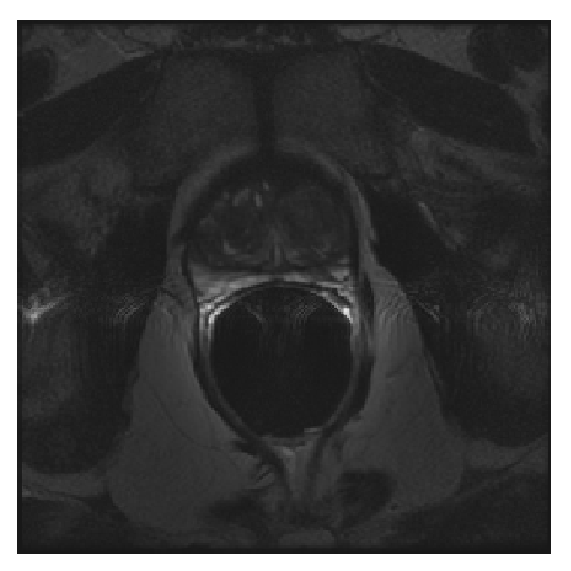
\includegraphics[width=0.3\linewidth]{3_review/figures/processing/pre-processing/bias/t2w_bias_antenna.eps}
	\caption[Inhomogeneity artefacts due to perturbation of the endorectal coil.]{Example of artefacts with high \ac{si} due to perturbation from the endorectal coil which create inhomogeneity.}
	\label{fig:bias}
\end{figure}

% Artefacts filtering
\item[$-$] \textbf{\textit{Bias correction:}} Besides being corrupted by noise, \ac{mri} images are also affected by the inhomogeneity of the \ac{mri} field commonly referred to as bias field \cite{Styner2000}.
This bias field results in a smooth variation of the \ac{si} through the image.
When an endorectal coil is used, an artefact resulting of an hyper-intense signal can be observed around the coil on the images (see Fig.~\ref{fig:bias}).

As a consequence, the \ac{si} of identical tissues varies depending on their spatial location in the image making further processes such as segmentation or registration harder \cite{Jungke1987,Vovk2007}.
A review of bias correction methods can be found in \cite{Vovk2007}.

{\color{blue}
The model of image formation is usually formalized such that:

\begin{equation}
	s(\mathbf{x}) = o(\mathbf{x})b(\mathbf{x}) + \eta(\mathbf{x}) \ ,
	\label{eq:biasmodel}
\end{equation}

\noindent where $s(\mathbf{x})$ is the corrupted \ac{si} at the pixel for the image coordinates $\mathbf{x} = \{x,y\}$, $o(\mathbf{x})$ is the ``noise-free signal'' , $b(\mathbf{x})$ is the bias field function and $\eta(\mathbf{x})$ is an additive white Gaussian noise.
%
%By using property of logarithm, the model of Eq. \eqref{eq:biasmodel} becomes additive such that:
%
%\begin{eqnarray}
%	\log s(\mathbf{x}) - \log b(\mathbf{x}) & = & \log \left( o(\mathbf{x}) + \frac{\eta(\mathbf{x})}{b(\mathbf{x})} \right) \ , \\ \nonumber
%	& = & \log \hat{o}(x) \ .
%\end{eqnarray}
%
%\noindent where $\hat{o}(\mathbf{x})$ is the signal only degraded by noise \cite{Styner2000}.

Hence, the task of bias correction involves estimating the bias function $b(\mathbf{x})$ in order to infer the ``signal-free bias'' $o(\mathbf{x})$.
% and subtract to the logarithm of the initial signal in order to obtain an estimated ``signal-free bias''.
}

Viswanath \textit{et al.}~\cite{Viswanath2009} performed bias correction on \ac{t2w}-\ac{mri} using a parametric Legendre polynomial model proposed in \cite{Styner2000} and available in the \ac{itk} library\footnote{The \ac{itk} library is available at: \texttt{http://www.itk.org/}}.

{\color{blue}
Styner \textit{et al.}~\cite{Styner2000} chose to model the bias field by using a linear combination of Legendre polynomials as:

\begin{equation}
	\hat{b}(\mathbf{x},\mathbf{p}) = \sum_{i=0}^{m-1} p_i f_i(\mathbf{x}) =  \sum_{i=0}^{l} \sum_{j=0}^{l-i} p_{ij} P_i(x) P_j(y) \ ,
	\label{eq:biascorr}
\end{equation}

\noindent where $\hat{b}$ is the bias estimation with the image coordinates $\mathbf{x} = \{x,y\}$ and the $m$ coefficients of the linear combination $\mathbf{p} = {p_{11},\dotsc,p_{ij}}$ ; $m$ can be defined as $m=(l+1)\frac{(l+2)}{2}$ where $l$ is the degree of Legendre polynomials chosen and $P_i(\cdot)$ denotes a Legendre polynomial of degree $i$.

This family of functions allows us to model the bias as a smooth inhomogeneity function across the image.
To estimate the set of parameters $\mathbf{p}$, a cost function is defined which relies on the following assumptions: (i) an image is composed of $k$ regions with $\mu_k$ being the mean \ac{si} and a variance $\sigma^{2}_{k}$ of each particular class, and (ii) each noisy pixel belongs to one of the $k$ regions with its \ac{si} value close to the class mean $\mu_k$.
Hence, the cost function is defined as:

\begin{equation}
	C(\mathbf{p}) = \sum_{\mathbf{x}} \prod_{k} \rho_k(s(\mathbf{x}) - \hat{b}(\mathbf{x},\mathbf{p}) - \mu_k) \ ,
	\label{eq:costbias}
\end{equation}

\begin{equation}
	\rho_k(x) = \frac{x^2}{x^2 + 3 \sigma_k^2} \ ,
	\label{eq:mestbias}
\end{equation}

\noindent where $\rho_k(\cdot)$ is a M-estimator allowing estimations to be less sensitive to outliers than usual square distance \cite{Li1996}.

Finally, estimation of the parameters $\mathbf{p}$ results in finding the minimum of the cost function $C(\mathbf{p})$.
This optimization was performed using the non-linear $(1+1)$ \ac{es} optimizer \cite{Styner1997}.

In a later publication, \cite{Viswanath2012} make use of the well known N3 algorithm\footnote{The N3 algorithm implementation is available at: \texttt{http://www.bic.mni.mcgill.ca/\allowbreak software/N3/}} to correct \ac{t2w}-\ac{mri} developed by \cite{Sled1998}.
To estimate the bias function, \cite{Sled1998} proposed to estimate the \acp{pdf} of the signal and bias.

Recalling Eq.~\eqref{eq:biasmodel} and taking advantage of logarithm property, it implies that this model becomes additive such that:

\begin{eqnarray}
	\log s(\mathbf{x}) & = & \log b(\mathbf{x}) + \log \left( o(\mathbf{x}) + \frac{\eta(\mathbf{x})}{b(\mathbf{x})} \right) \ , \nonumber \\
	& \approx & \log b(\mathbf{x}) + \log \hat{o}(\mathbf{x}) \ , \label{eq:logbias}
\end{eqnarray}

\noindent where $\hat{o}(\mathbf{x})$ is the signal only degraded by noise. \cite{Sled1998} shows that Eq. \eqref{eq:logbias} can be related to \acp{pdf} such that:

\begin{equation}
	S(s) = B(s) * O(s) \ ,
	\label{eq:distrbias} 
\end{equation}

\noindent where $S$, $B$ and $O$ are respectively the probability densities of $s$, $b$ and $o$.

Restoring the corrupted signal $s$ is carried out by finding the multiplicative field $b$ which maximizes the frequency content of the distribution $O$.
Sled \textit{et al.}~\cite{Sled1998} argue that a search through all possible fields $b$ and selection of the one which maximizes the high frequency content of $O$ could be carried out but results in an exhaustive search.
However, they show that the bias field distribution can be assimilated to a near Gaussian distribution.
Using this fact as \textit{a priori}, it is then possible to infer the distribution $O$ using Wiener deconvolution given $B$ and $S$ and later estimate the corresponding smooth field $b$.
}

Lv \textit{et al.}~\cite{Lv2009} corrected the inhomogeneity in \ac{t2w}-\ac{mri} images by using the method proposed in \cite{Madabhushi2006}.
In this method, the \ac{mri} images are corrected iteratively by successively detecting the image foreground via \ac{gscale} and estimating a bias field function based on a second-order polynomial model. 
{\color{blue}
First the background of the \ac{mri} image is eliminated by threholding.
The threshold value is commonly equal to the mean \ac{si} of the considered image.
Then, in the seeded region growing algorithm is applied considering every thresholded pixel as a potential seed.
However, pixels already assigned to a region will not be considered any more as seed.
As in seeded region growing algorithm \cite{Shapiro2001}, two criteria are taken into account to expand the region.
First, the region will grow using a connected-neighbourhood, initially defined by the user.
Then, the homogeneity of \ac{si} is based on a fuzzy membership function taking into account the absolute difference of the \acp{si} of two pixels.
Depending on the membership value (cf., a threshold has to be defined), the pixel considered is merged or not to the region.
Once this segmentation is performed, the largest region $R$ is used as a mask to select pixels of the original image and the mean \ac{si}, $\mu_{R}$, is computed. 
The background variation $b(\mathbf{x})$ is estimated as:

\begin{equation}
	b(\mathbf{x}) = \frac{s(\mathbf{x})}{\mu_{R}}, \ \forall \mathbf{x} \in R \ ,
	\label{eq:backest}
\end{equation}

\noindent where $s(\mathbf{x})$ is the original \ac{mri} image.

Finally, a second order polynomial $\hat{b}_{\Theta}(\mathbf{x})$ is fitted in a least-squares sense (Eq.~\eqref{eq:lsolv}),

\begin{equation}
	\hat{\Theta} = \argmin_{\Theta} | b(\mathbf{x}) - \hat{b}_{\Theta}(\mathbf{x}) |^{2}, \ \forall \mathbf{x} \in R \ .
	\label{eq:lsolv}
\end{equation}

Finally, the whole original \ac{mri} image is corrected by dividing it by the estimated bias field function $\hat{b}_{\Theta}(\mathbf{x})$.
This process is repeated until the number of pixels in the largest region $R$ does not change significantly between two iterations.
}

%SI normalization
\item[$-$] \textbf{\textit{\Ac{si} normalization/standardization:}}

As discussed in the later section, segmentation or classification tasks are usually performed by first learning from a training set of patients.
Hence, one can emphasize the desire to perform \ac{mri} examinations with a high repeatability or in other words, one would ensure to obtain similar \ac{mri} images (cf., similar \acp{si}) for patients of the same group (cf., healthy patients \textit{vs.} patients with \ac{cap}), for a similar sequence.

However, it is a known fact that variability between patients occurs during the \ac{mri} examinations even using the same scanner, protocol or sequence parameters \cite{Nyul1999}.
Hence, the aim of normalization or standardization of the \ac{mri} data is to remove the variability between patients and enforce the repeatability of the \ac{mri} examinations.
Approaches used to standardize \ac{mri} images can be either categorized as statistical-based standardization or organ \ac{si}-based standardization. 

Artan \textit{et al.}~\cite{Artan2009,Artan2010} as well as Ozer \textit{et al.}~\cite{Ozer2009,Ozer2010} standardized \ac{t2w}, \ac{dce} and \ac{dw} \ac{mri} images by computing the \textit{standard score} (also called \textit{z-score}) of the pixels of the \ac{pz} as:

\begin{equation}
	I_s(\mathbf{x}) = \frac{ I_r(\mathbf{x}) - \mu_{pz}}{\sigma_{pz}}, \ \forall \mathbf{x} \in \text{PZ} \ ,
	\label{eq:meansta}
\end{equation}

\noindent where $I_s(\mathbf{x})$ is the standardized \ac{si} with the image coordinates $\mathbf{x} = \{x,y\}$, $I_r(\mathbf{x})$ is the raw \ac{si}, $mu_{pz}$ is the mean-\ac{si} of the \ac{pz} and $\sigma_{pz}$ is the \ac{si} standard deviation in the \ac{pz}.
This transformation enforces the image \ac{pdf} to have a zero mean and a unit standard deviation.

In a similar way, Liu \textit{et al.}~\cite{Liu2013} normalized \ac{t2w}-\ac{mri} by making use of the median and interquartile range for all the pixels.

Lv \textit{et al.}~\cite{Lv2009} scaled the \ac{si} of \ac{t2w}-\ac{mri} images using the method proposed in \cite{Nyul2000} based on \ac{pdf} matching.
This approach is based on the assumption that \ac{mri} images from the same sequence should share the same \ac{pdf} appearance.
Hence, one can approach this issue by transforming and matching the \acp{pdf} using some statistical landmarks such as median and different quantiles.
Using a training set, these statistical landmarks are extracted for $N$ training images as for instance for the minimum, the $25^{\text{th}}$ quantile, the median, the $75^{\text{th}}$ quantile and the maximum:

\begin{eqnarray}	
	\Phi_{0} & = & \{ \phi_{0}^{1}, \phi_{0}^{2}, \cdots, \phi_{0}^{N} \} \ , \nonumber \\
	\Phi_{25} & = & \{ \phi_{25}^{1}, \phi_{25}^{2}, \cdots, \phi_{25}^{N} \} \ , \nonumber \\
	\Phi_{50} & = & \{ \phi_{50}^{1}, \phi_{50}^{2}, \cdots, \phi_{50}^{N} \} \ ,  \label{eq:quantileStd} \\
	\Phi_{75} & = & \{ \phi_{75}^{1}, \phi_{75}^{2}, \cdots, \phi_{75}^{N} \} \ , \nonumber \\
	\Phi_{100} & = & \{ \phi_{100}^{1}, \phi_{100}^{2}, \cdots, \phi_{100}^{N} \} \ , \nonumber
\end{eqnarray}

\noindent where $\phi_{n^\text{th}}^{i^{\text{th}}}$ is the $n^{\text{th}}$ quantile of the $i^{\text{th}}$ training image.

\begin{figure}
	\centering
	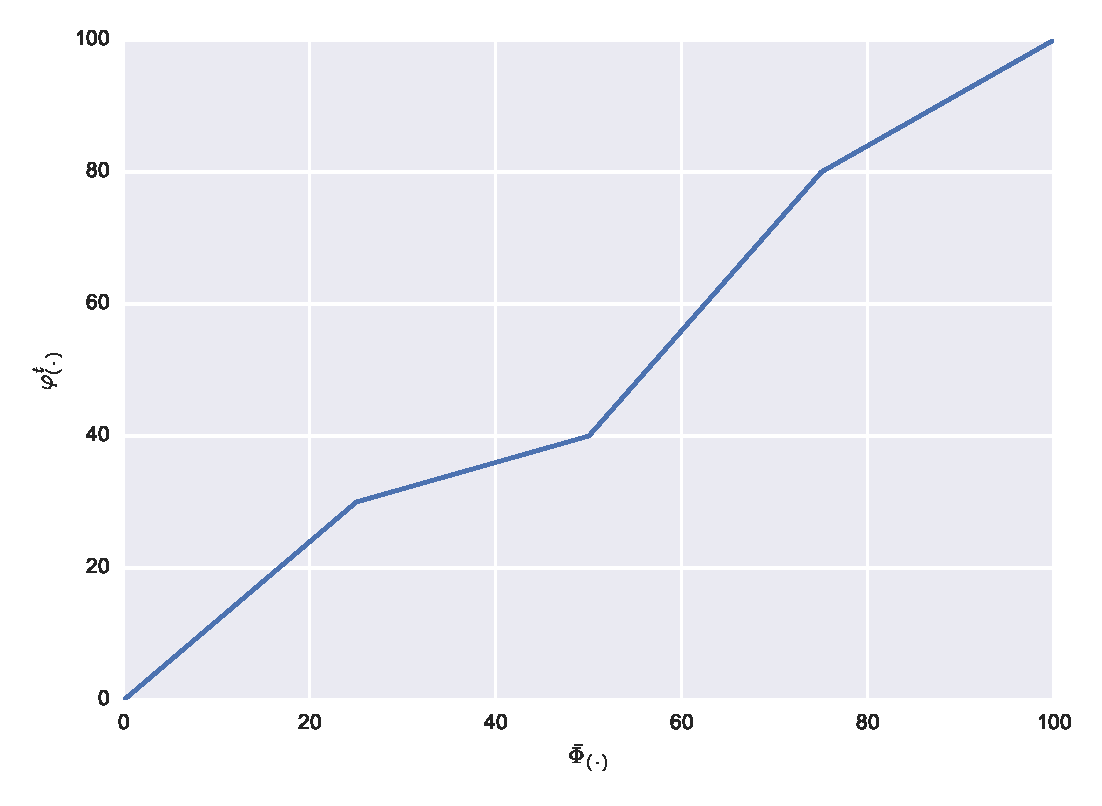
\includegraphics[width=0.7\linewidth]{3_review/figures/processing/pre-processing/normalization/linear_transform_parts.eps}
	\caption{Example of linear mapping by parts as proposed by \cite{Nyul2000}.}
	\label{fig:imnorm}
\end{figure}

Then, the mean of each quantile $\{ \bar{\Phi}_{0}, \bar{\Phi}_{25}, \bar{\Phi}_{50}, \bar{\Phi}_{75}, \bar{\Phi}_{100} \}$ is also calculated.
Once this training stage is performed, a linear transformation by parts $\mathcal{T}(\cdot)$ can be computed (Eq.~\eqref{eq:linearMap}) for each test image $t$ by mapping each statistical landmark $\varphi_{(cdot)}̂^{t}$ of this image with the pre-learned statistical landmarks $\bar{\Phi}_{(\cdot)}$.
This linear mapping is also depicted in Fig.~\ref{fig:imnorm}.

\begin{equation}
\small
\mathcal{T}(s(\mathbf{x})) =
  \begin{cases}
    \lceil \bar{\Phi}_{0}+( s(\mathbf{x}) - \varphi_{0}^{t} ) \left( \frac{\bar{\Phi}_{25} - \bar{\Phi}_{0}}{\varphi_{25}^{t} - \varphi_{0}^{t}} \right) \rceil \ , & \text{if $\varphi_{0}^{t} \leq s(\mathbf{x})<\varphi_{25}^{t})$} \ , \\
    \lceil \bar{\Phi}_{25}+( s(\mathbf{x}) - \varphi_{25}^{t} ) \left( \frac{\bar{\Phi}_{50} - \bar{\Phi}_{25}}{\varphi_{50}^{t} - \varphi_{25}^{t}} \right) \rceil \ , & \text{if $\varphi_{25}^{t} \leq s(\mathbf{x})<\varphi_{50}^{t})$} \ , \\
    \lceil \bar{\Phi}_{50}+( s(\mathbf{x}) - \varphi_{50}^{t} ) \left( \frac{\bar{\Phi}_{75} - \bar{\Phi}_{50}}{\varphi_{75}^{t} - \varphi_{50}^{t}} \right) \rceil \ , & \text{if $\varphi_{50}^{t} \leq s(\mathbf{x})<\varphi_{75}^{t})$} \ , \\
    \lceil \bar{\Phi}_{75}+( s(\mathbf{x}) - \varphi_{75}^{t} ) \left( \frac{\bar{\Phi}_{100} - \bar{\Phi}_{75}}{\varphi_{100}^{t} - \varphi_{75}^{t}} \right) \rceil \ , & \text{if $\varphi_{75}^{t} \leq s(\mathbf{x})\leq \varphi_{100}^{t})$} \ ,
  \end{cases}
  \label{eq:linearMap}
\end{equation}

Viswanath \textit{et al.}~\cite{Viswanath2009,Viswanath2011,Viswanath2012} use a variant of this previous approach presented in \cite{Madabhushi2006a} aiming to standardize the \ac{t2w}-\ac{mri} images.Instead of computing the \ac{pdf} of an entire image, a pre-segmentation of the foreground is carried out via \ac{gscale} which was discussed in the bias correction section.
Once the foreground is detected, the largest region is extracted and the same process than previously mentioned (see Eq.~\eqref{eq:linearMap}) takes place in order to align \acp{pdf} of the foreground of the \ac{mri} images.

\begin{figure}
\centering
	\hspace*{\fill}
	\subfigure[Illustration and location of the bladder on a \ac{t2w}-\ac{mri} image acquired with a 3.0 Tesla \ac{mri} scanner]{\label{subfig:bladder} 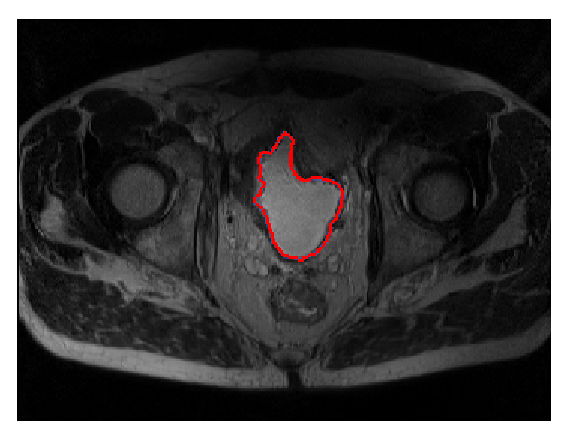
\includegraphics[width=0.3\linewidth]{3_review/figures/processing/pre-processing/niaf/t2w_bladder.eps}} \hfill
	\subfigure[Illustration and location of the femoral arteries on a \ac{t1w}-\ac{mri} image acquired with a 3.0 Tesla \ac{mri} scanner]{\label{subfig:arteries} 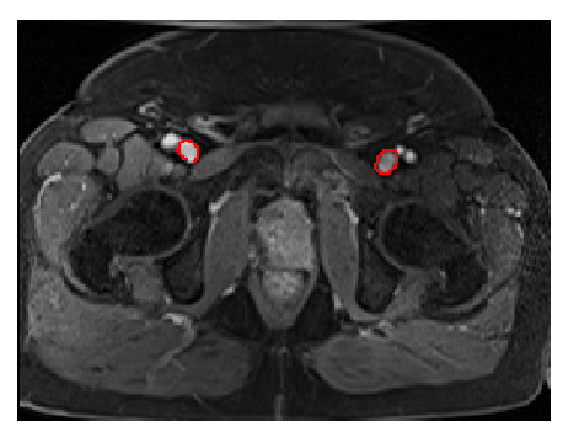
\includegraphics[width=0.3\linewidth]{3_review/figures/processing/pre-processing/niaf/t1w_arteries.eps}}
	\hspace*{\fill}
	\caption{Illustration of the two organs used by \cite{Niaf2011,Niaf2012} to normalize \ac{t2w} and \ac{t1w} \ac{mri} images.}
	\label{fig:niaf}
\end{figure}

The methods described above were statistical-based methods.
However, the standardization problem can be tackled by normalizing the MRI images using the \ac{si} of some known organs present in these images. 
Niaf \textit{et al.}~\cite{Niaf2011,Niaf2012} normalized \ac{t2w}-\ac{mri} images by dividing the original \ac{si} of the images by the mean \ac{si} of the bladder (see Fig.~\ref{subfig:bladder}).
Likewise, \cite{Niaf2011} standardized the \ac{t1w}-\ac{mri} images using the \ac{aif}.
They computed the \ac{aif} by taking the mean of the \ac{si} in the most enhanced part of the common femoral arteries (see Fig. \ref{subfig:arteries}) as proposed in \cite{Wiart2007}.

\end{enumerate}


Presented in Sect.~\ref{subsec:chp2:imaging:mrsi}, \ac{mrsi} is a modality related to a one dimensional signal.
Hence, specific pre-processing steps for this type of signals have been applied instead of standard signal processing methods.

\setenumerate{listparindent=\parindent,itemsep=10px}
\setlist{noitemsep}
\begin{enumerate}[leftmargin=*]

\begin{figure}
	\centering
	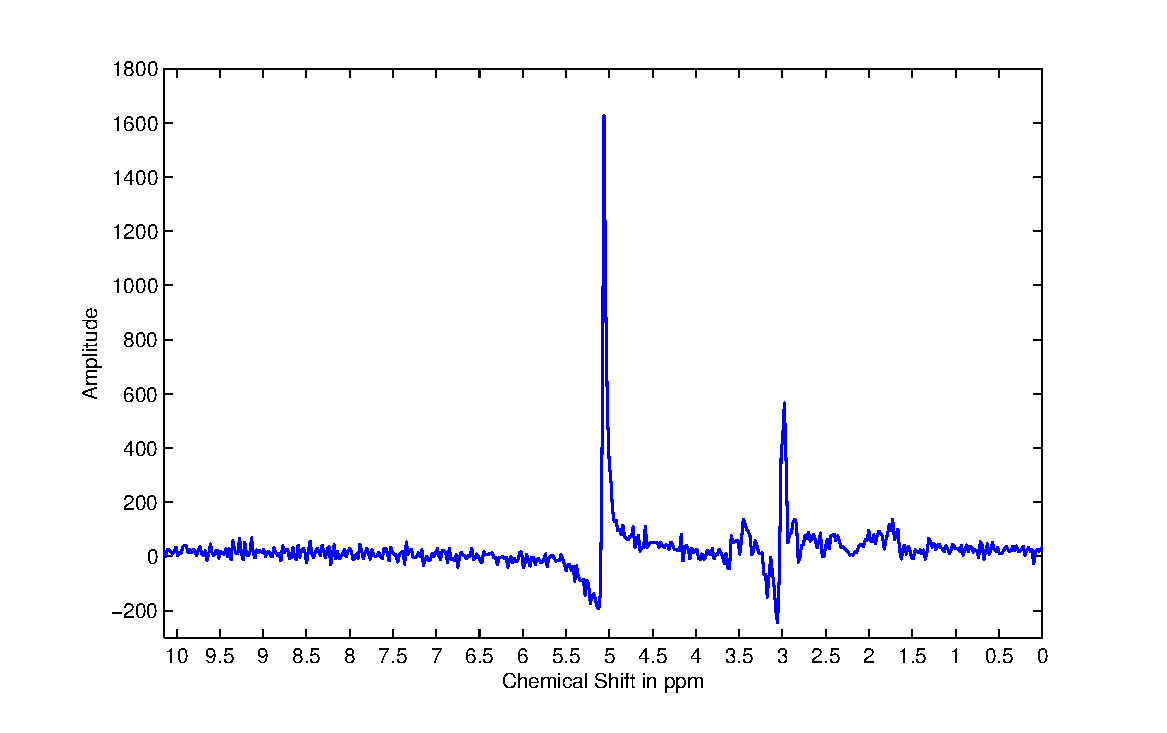
\includegraphics[width=0.7\linewidth]{3_review/figures/processing/pre-processing/phase/phase.eps}
	\caption[Illustration of phase malignant in an \ac{mrsi} spectra.]{Illustration of phase misalignment in an \ac{mrsi} spectra acquire with a 3.0 Tesla \ac{mrsi} scanner. Note the distortion of the signal specially visible for the water and citrate peaks.}
	\label{fig:phase}
\end{figure}

	\item[$-$] \textbf{\textit{Phase correction:}} \ac{mrsi} data acquired suffer from zero-order and first-order phase misalignments as shown in Fig.~\ref{fig:phase} \cite{Chen2002,Osorio-Garcia2012}. 
Parfait \textit{et al.}~\cite{Parfait2012} used a method proposed in \cite{Chen2002} where the phase of \ac{mrsi} signal is corrected based on entropy minimization in the frequency domain.
The corrected \ac{mrsi} signal $o(\xi)$ can be expressed as:

\begin{eqnarray}
	\Re(o(\xi)) & = & \Re(s(\xi))\cos(\Phi(\xi)) - \Im(\xi)\sin(\Phi(\xi)) \ , \nonumber  \\
	\Im(o(\xi)) & = & \Im(s(\xi))\cos(\Phi(\xi)) + \Re(\xi)\sin(\Phi(\xi)) \ , \nonumber \\
	\Phi(\xi) & = & \phi_0 + \phi_1 \frac{\xi}{N} \ , \label{eq:mrsiphcorr}
\end{eqnarray}

\noindent where $\Re(\cdot)$ and $\Im(\cdot)$ are the real and imaginary part of the complex signal respectively, $s(\xi)$ is the corrupted \ac{mrsi} signal, $\phi_0$ and $\phi_1$ are the zero-order and first-order phase correction terms respectively and $N$ is the total number of samples of the \ac{mrsi} signal.

Chen \textit{et al.}~\cite{Chen2002} tackled this problem using an optimization framework where $\phi_0$ and $\phi_1$ had to be inferred.
Hence, the simplex Nelder-Mead optimization method was used to minimize the following cost function based on the \textit{Shannon entropy} formulation:

\begin{equation}
	\hat{\Phi} = \argmin_{\Phi} \left[ - \sum \Re(s'(\xi)) \ln \Re(s'(\xi)) + \lambda \|\Re(s(\xi))\|_2 \right] \ ,
	\label{eq:phcost}
\end{equation}

\noindent where $s'(\xi)$ is the first derivative of the corrupted signal $s(\xi)$ and $\lambda$ is a regularization parameter.
Once the best parameter $\Phi$ is obtained, the \ac{mrsi} signal is corrected using Eq.~\eqref{eq:mrsiphcorr}.

\begin{figure}
\centering
	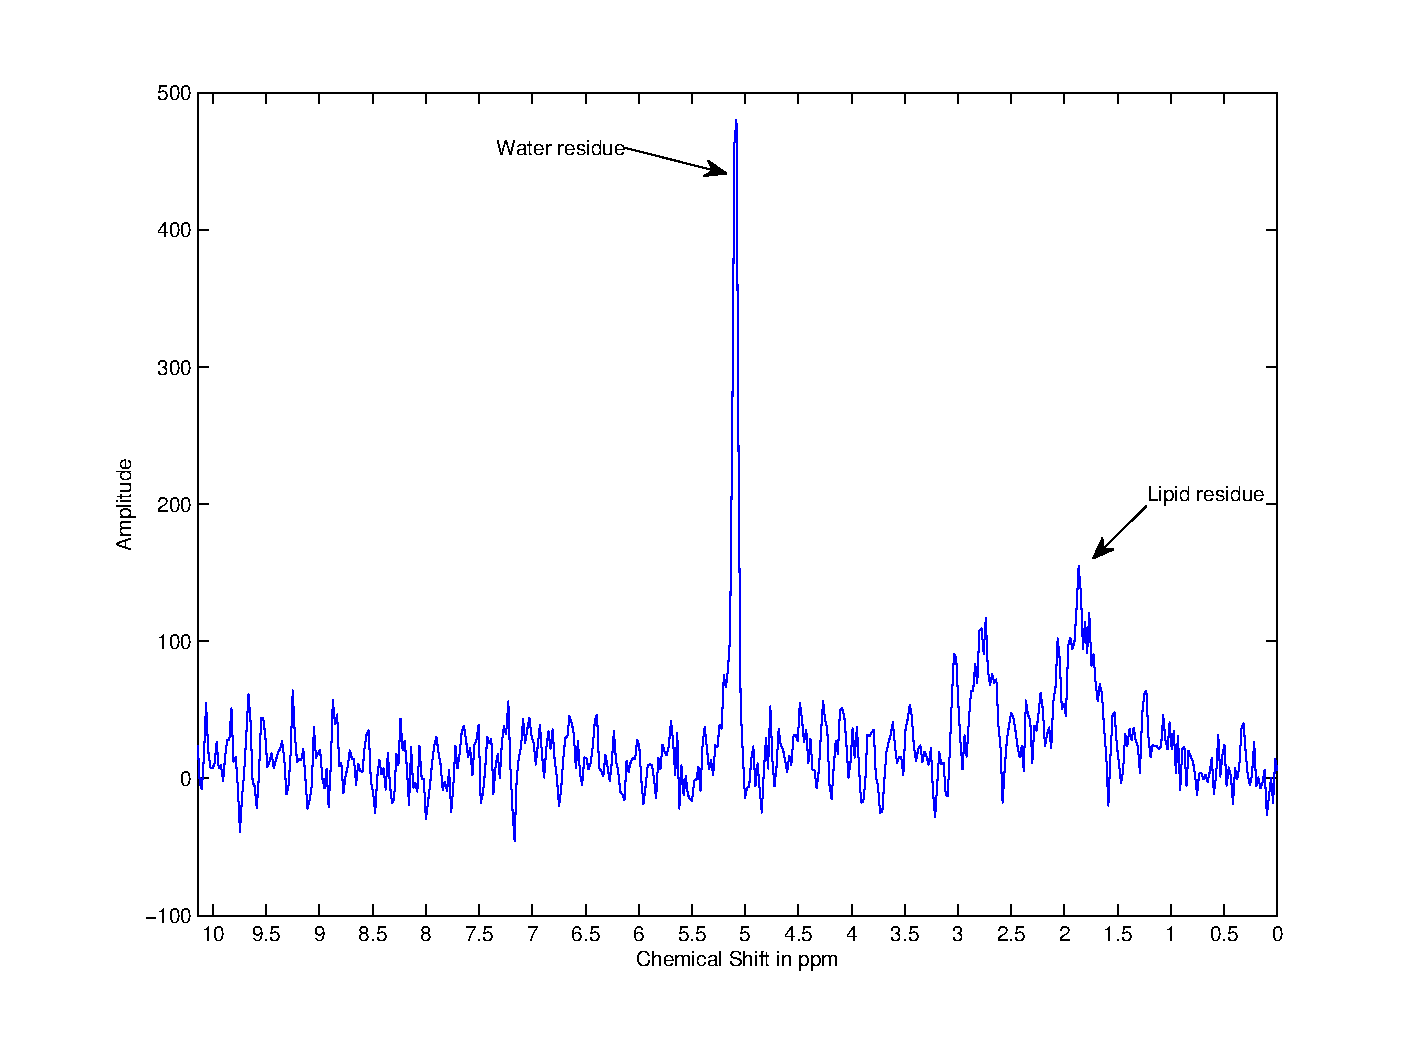
\includegraphics[width=0.7\linewidth]{3_review/figures/processing/pre-processing/water/water_fat.eps}
	\caption[Illustration of water and fat residues in \ac{mrsi} signal after supression during acquisition.]{Illustration of the residues of water and fat even after their suppression during the acquisition protocol. The acquisition was carried out with a 3.0 Tesla \ac{mri}.}
	\label{fig:waterfat}
\end{figure}

	\item[$-$] \textbf{\textit{Water and lipid residuals filtering:}} The water and lipid metabolites occur in much higher concentrations the metabolites of interests (cf., choline, creatine and citrate) \cite{Zhu2010,Osorio-Garcia2012}.
Fortunately, specific \ac{mrsi} sequences were developed in order to suppress water and lipid metabolites using pre-saturation techniques \cite{Zhu2010}.
However, these techniques do not perfectly remove water and lipids peaks and some residuals are still present in the \ac{mrsi} spectra as shown in Fig.~\ref{fig:waterfat}.
Therefore, different post-processing methods have been proposed to enhance the quality of the \ac{mrsi} spectra by removing these residuals.
For instance, Kelm \textit{et al.}~\cite{Kelm2007} used the well known HSVD algorithm proposed by \cite{Pijnappel1992} which models the \ac{mrsi} signal by a sum of exponentially damped sinusoids in the time domain (see Eq.~\eqref{eq:fidsig}).
%In the time domain, a \ac{mrsi} signal $s(t)$ is modelled by a sum of $K$ exponentially damped sinusoids such that:

\begin{equation}
	s(t) = \sum_{k=1}^{K} a_{k}\exp(i \phi_k) \exp( -d_{k} + i 2 \pi f_{k} ) t + \eta(t) \ ,
	\label{eq:fidsig}
\end{equation}

\noindent where $a_k$ is the amplitude proportional to the metabolite concentration with a resonance frequency $f_{k}$, $d_k$ represents the damping factor of the exponential, $\phi_k$ is the first-order phase and $\eta(t)$ is a complex white noise. 

Pijnappel \textit{et al.}~\cite{Pijnappel1992} showed that the ``noise-free signal'' can be found using the \ac{svd} decomposition.
First the noisy signal is reorganized inside a Hankel matrix $H$.
It can be shown that if the signal considered would be a ``noise-free signal'', the rank of $H$ would be equal to rank $K$.
However, due to the presence of noise, $H$ is in fact a full rank matrix.
Thus, to recover the ``noise-free signal'', the rank of $H$ can be truncated to $K$ using its \ac{svd} decomposition.
Hence, knowing the cut off frequencies of water (cf., 4.7 ppm) and lipid (cf., 2.2 ppm) metabolites, their corresponding peaks can be reconstructed and subtracted from the original signal \cite{Laudadio2002}.
	
	\item[$-$] \textbf{\textit{Baseline correction:}} Sometimes, the problem discussed in the above section regarding the lipid molecules is not addressed simultaneously with water residuals suppression.
Lipids and macromolecules are known to affect the baseline of the \ac{mrsi} spectra.
They could cause errors during further fitting processes aiming to quantify the metabolites, especially regarding the citrate metabolite.
	
Parfait \textit{et al.}~\cite{Parfait2012} made the comparison of two different methods to detect the baseline and correct the \ac{mrsi} spectra which are based on \cite{Lieber2003,Devos2004}. 
Lieber \textit{et al.}~\cite{Lieber2003} addressed the problem of baseline detection in the frequency domain by fitting a low degree  polynomial whereas Parfait \textit{et al.}~\cite{Parfait2012} modified this algorithm by convolvinga Gaussian kernel to smooth the \ac{mrsi} signal instead of fitting a polynomial function.
{\color{red} \textbf{Check the tex file to see the commented area pre-processing.tex}}
%% of low degree $p(x)$ (e.g., second or third degree) to the \ac{mrsi} signal $s(x)$ in a least-squares sense.
%% Then, the values of the fitted polynomial are re-assigned as:

%% \begin{equation}
%% 	p_f(x) = 
%% 	\begin{cases}
%% 		p(x) \ , & \text{if $p(x) \leq s(x)$} \ , \\
%% 		s(x) \ , & \text{if $p(x) > s(x)$} \ . \\
%% 	\end{cases}
%% 	\label{eq:lieber}
%% \end{equation}

%% Finally, this procedure of fitting and re-assignment is iteratively repeated on $p_f(x)$ until a stopping criterion is reached. The final polynomial function can be subtracted from the original signal s(x) to correct it.

%% \cite{Parfait2012} modified this algorithm by convolving a Gaussian kernel to smooth the \ac{mrsi} signal instead of fitting a polynomial function, keeping the rest of the algorithm identical. 
Unlike in \cite{Lieber2003}, Devos \textit{et al.}~\cite{Devos2004} proposed to correct the baseline in the time domain by multiplying the \ac{mrsi} signal by a decreasing exponential function as:
\begin{equation}
	c(t) = \exp (- \beta t) \ ,
	\label{eq:devos}
\end{equation}

\noindent Having a typical value for $\beta$ of 0.15.
However, Parfait \textit{et al.}~\cite{Parfait2012} concluded that the method proposed in \cite{Lieber2003} outperformed the one in \cite{Devos2004}.

In the contemporary work of Tiwari \textit{et al.}~\cite{Tiwari2012}, the authors detected the baseline using a local non-linear fitting method avoiding regions with significant peaks which were detected using a experimentally parametrised signal-to-noise ratio (i.e. a value larger than 5 dB).


\begin{figure}
\centering
	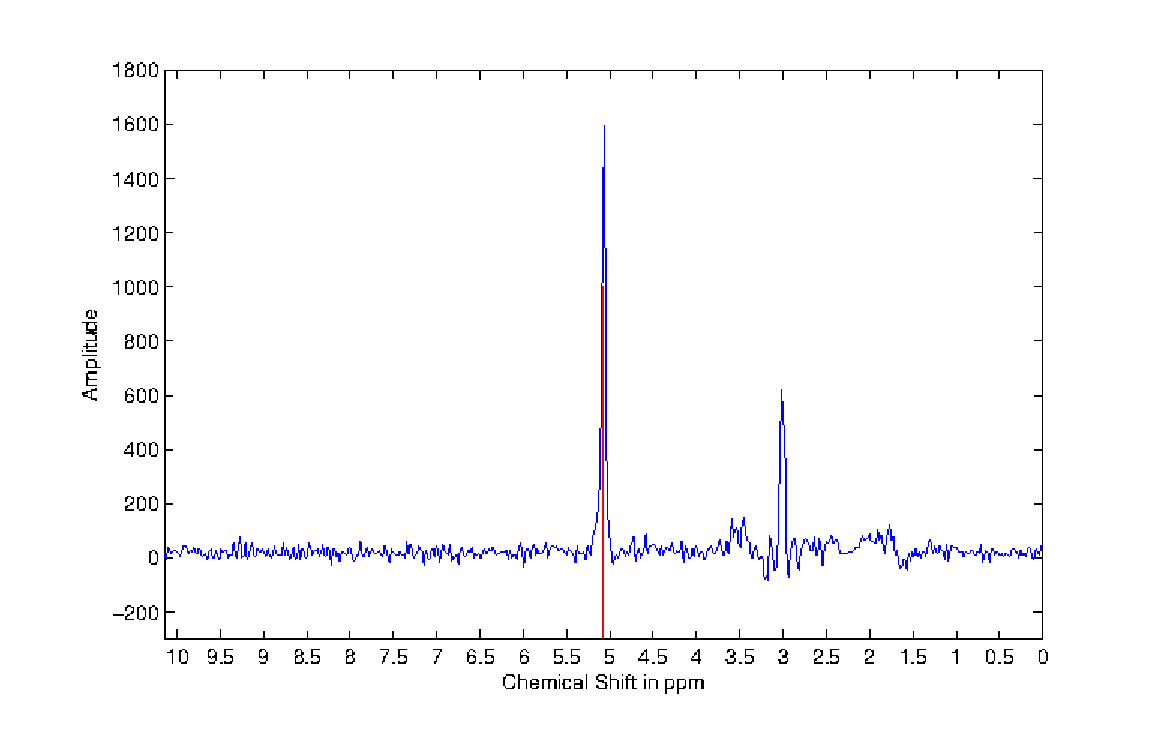
\includegraphics[width=0.7\linewidth]{3_review/figures/processing/pre-processing/frequency/frequency.eps}
	\caption[Illustration of frequency misalignment in an \ac{mrsi} spectra.]{Illustration of frequency misalignment in an \ac{mrsi} spectra acquired with a 3.0 Tesla \ac{mrsi} scanner. The water peak is known to be aligned at 4.65 ppm. However, it can be seen that the peak on this spectra is aligned at around 5.1 ppm.}
	\label{fig:frequency}
\end{figure}

	\item[$-$] \textbf{\textit{Frequency alignment:}} Due to variations of the experimental conditions, a frequency shift can be observed in the \ac{mrsi} spectra \cite{Chen2002,Osorio-Garcia2012} as shown in Fig.~\ref{fig:frequency}.
	
Tiwari \textit{et al.}~\cite{Tiwari2012} corrected the frequency shift by first detecting known metabolite peaks such as choline, creatine and citrate.
The frequency shift is corrected by minimizing the frequency error between the experimental and theoretical values of each of these peaks.

	\item[$-$] \textbf{\textit{Normalization:}} Due to variations of the experimental conditions, the \ac{mrsi} signal may also vary between patients.
Parfait \textit{et al.}~\cite{Parfait2012} as in \cite{Devos2004} compared two methods to normalize \ac{mrsi} signal.
In each method, the original \ac{mrsi} spectra is divided by a normalization factor, similar to the intensity normalization described earlier.  
The first approach to obtain the normalization factor is based on an estimation of the water concentration.
It is required to have an additional \ac{mrsi} sequence where the water metabolites are unsuppressed.
Using this sequence, an estimation of the water concentration can be performed using the previously reported HSVD algorithm.
The second approach to normalization is based on using the L$_2$ norm of the \ac{mrsi} spectra $\|s(\xi)\|_2$. 
It should be noted that both \cite{Parfait2012} and \cite{Devos2004} concluded that the L$_2$ normalization was more efficient in their framework.
 
\end{enumerate}


\begin{table}
	\caption{Overview of the pre-processing methods used in \ac{cad} systems.}
	\small
	%\renewcommand{\arraystretch}{1.5}
	\begin{tabular}{p{.65\linewidth} p{.25\linewidth}}
		\hline \\ [-1.5ex]
		\textbf{Pre-processing operations} & \textbf{References} \\ \\ [-1.5ex]
		\hline \\ [-1.5ex]
		\textit{\ac{mri} pre-processing:} & \\ \\ [-1.5ex]
		\quad Noise filtering: &  \\
		\quad \quad Median filtering & $[$20-21$]$  \\
		\quad \quad Wavelet-based filtering & $[$1-2,14$]$ \\ \\ [-1.5ex]
		\quad Bias correction: & \\
		\quad \quad Parametric methods & $[$15-35$]$ \\
		\quad \quad Non-parametric methods & $[$36$]$ \\ \\ [-1.5ex]
		\quad Standardization: & \\
		\quad \quad Statistical-based normalization: & $[$3-4,15,20-21,35,37$]$ \\
		\quad \quad Organ \ac{si}-based normalization & $[$18-19$]$ \\ \\ [-1.5ex]
		\textit{\ac{mrsi} pre-processing:} & \\ \\ [-1.5ex]
		\quad Phase correction & $[$22$]$ \\
		\quad Water and lipid residuals filtering & $[$8$]$ \\
		\quad Baseline correction & $[$22,31$]$ \\
		\quad Frequency alignment & $[$31$]$ \\
		\quad Normalization & $[$22$]$ \\ \\ [-1.5ex]
		\hline
	\end{tabular}
\label{tab:summary-preproc}
\end{table}

\subsection{Segmentation}\label{subsec:chp3:img-reg:seg}
The segmentation task consists in delineating the prostate boundaries in the \ac{mri} and is of particular importance for focusing the posterior processing on the organ of interest~\cite{Ghose2012}. 
In this section, only the segmentation methods used in \ac{cad} for \ac{cap} are presented.
An exhaustive review of prostate segmentation methods in \ac{mri} is available in~\cite{Ghose2012}.

%% \setenumerate{listparindent=\parindent,itemsep=10px}
%% \setlist{noitemsep}
%% \begin{enumerate}[leftmargin=*]

%\item[$-$] \textbf{\textit{Manual segmentation:}} 
\paragraph{Manual segmentation}
To highlight the importance of prostate segmentation task in \ac{cad} systems, it is interesting to note the large number of studies which manually segment the prostate organs~\cite{Artan2009,Artan2010,Matulewicz2013,Niaf2011,Niaf2012,Ozer2009,Ozer2010,Puech2009,Vos2008,Vos2008a,trigui2016classification,trigui2017automatic,lehaire2014computer}.
In all the cases, the boundaries of the prostate gland are manually defined in order to limit further processing to only this area.
This approach ensures the right delineation of the organ; nevertheless this procedure is highly time consuming and should be performed by a radiologist.

%\item[$-$] \textbf{\textit{Region-based segmentation:}} 
\paragraph{Region-based segmentation}
\citeauthor{Litjens2012} used a multi-atlas-based segmentation using multi-modal images --- i.e., \ac{t2w}-\ac{mri} and \ac{adc} map --- to segment the prostate with an additional pattern recognition method to differentiate \ac{cg} and \ac{pz}~\cite{Litjens2012}, as proposed in~\cite{Litjens2012a}.
This method consists in three different steps: (i) the registration between each atlas and the multi-modal images, (ii) the atlas selection, and finally (iii) the classification of the prostate voxels into either \ac{cg} or \ac{pz} classes.
Each atlas and the \ac{mri} images are registered two successive registrations: a rigid registration to roughly align the atlases and the \ac{mri} images followed by an elastic registration using a B-spline transformation.
The cost function driving the registration is defined as the weighted sum of the \ac{mi} of both \ac{t2w}-\ac{mri} and \ac{adc} map.
The final atlas is selected using either a majority voting or the \ac{staple} approach~\cite{Warfield2004}.
Subsequently, each voxel within the prostate are classified either as \ac{cg} or \ac{pz} using a \ac{lda} classifier.
Three types of feature are considered to characterized the voxels: (i) anatomy, (ii) intensity, and (iii) texture.
The relative position and the relative distance from the voxel to the border of the prostate encode the anatomical information.
The intensity features consist in the intensity of the voxel in the \ac{adc} coefficient and the T$_2$ map.
The texture features are composed of 5 different features: homogeneity, correlation~\cite{Amadasun1989}, entropy, texture strength~\cite{Li2005a}, and \ac{lbp}~\cite{Ojala1996}.
Finally, the final segmentation is obtained by removing artifacts and smoothing the contour between the zones using the \ac{tps}~\cite{Bookstein1989}.

\citeauthor{Litjens2014} used an almost identical algorithm in~\cite{Litjens2014}, initially proposed for the PROMISE12 challenge~\cite{Litjens2014a}.
Their segmentation method is also based on multi-atlas multi-modal images, but the SIMPLE method~\cite{langerak2010label} is used instead, to combine labels after the registration of the different atlas to obtain the final segmentation.
 
Finally, \citeauthor{rampun2016computerb} recurrently used a method to segment the \ac{pz}~\cite{rampun2015classifying,rampun2015computer,rampun2016computer,rampun2016computerb,rampun2016quantitative}, which is proposed in~\cite{rampun2014detection}.
The \ac{pz} is modelled using a quadratic function driven by the centre of the prostate, the left-most, and the right-most coordinates of the prostate boundaries.

%\item[$-$] \textbf{\textit{Model-based segmentation:}} 
\paragraph{Model-based segmentation}
\citeauthor{Viswanath2009} in~\cite{Viswanath2008a,Viswanath2009} used the \ac{mantra} method as proposed by \citeauthor{Toth2008}.
\ac{mantra}~\cite{Toth2008} is closely related to the \ac{asm} from~\cite{Cootes1995}.
This algorithm consists of two stages: (i) a training stage where a shape and an appearance model are generated and (ii) the actual segmentation based on the learned model. 
For the training stage, a set of landmarks is defined and the shape model is generated as in the original \ac{asm} method~\cite{Cootes1995}.
Then, to model the appearance, a set of $K$ texture images $\{I_1,I_2,\cdots,I_k\}$ based on first and second order statistical texture features is computed.
For a given landmark $l$ with its given neighbourhood $\mathcal{N}(l)$, its feature matrix extracted is expressed as:

\begin{equation}
  f_l = \{ I_1(\mathcal{N}(l)), I_2(\mathcal{N}(l)), \cdots, I_k(\mathcal{N}(l)) \} \ ,
  \label{eq:mantra1}
\end{equation}

\noindent where $I_k(\mathcal{N}(l))$ represents a feature vector obtained by sampling the $k^{\text{th}}$ texture map using the neighbourhood $\mathcal{N}(l)$.
Therefore, multiple landmarks are generated followed by a decomposition using \ac{pca}~\cite{Pearson1901} to learn the appearance variations as in \ac{asm}.

For the segmentation stage, the mean shape learned previously is initialized in the test image.
The same associated texture images as in the training stage are computed.
For each landmark $l$, a neighbourhood of patches are used to sample the texture images and a reconstruction is obtained using the appearance model previously trained.
The new landmark location will be defined as the position where the \ac{mi} is maximal between the reconstructed and original values.
This scheme is performed in a multi-resolution manner as in \cite{Cootes1995}.

Subsequently, \citeauthor{Viswanath2012} in~\cite{Viswanath2012}, used the \ac{weritas} method also proposed in~\citeauthor{Toth2009}.
Similarly to \ac{mantra}, \ac{weritas} is also based on the \ac{asm} formulation~\cite{Toth2009}.
%As with the \ac{mantra} method, \ac{weritas} is based on the \ac{asm} formulation.
%In fact it is very close to the \ac{mantra} itself. 
%The same texture features are used to construct the appearance models, but instead of using \ac{mi} between the landmarks and neighbour patches for adapting the landmark positions, it defines a metric based on the Mahalanobis distance.
They differ in the last stage of the algorithm in which the Mahalanobis distance is used instead of the \ac{mi} metric, to adapt the positions of new landmarks.
In the training stage, the Mahalanobis distance is computed between landmarks and neighbour patches for each of the features.
Subsequently, a new metric is proposed as a linear weighted combination of those Mahalanobis distances which maximizes the correlation with the Euclidean distance between the patches and the true landmarks.
In the segmentation step, this metric is then computed between the initialized landmarks and neighbouring patches in order to update landmark positions, in a similar fashion to other \ac{acm} models.

\citeauthor{Litjens2011} as well as \citeauthor{Vos2012} used an approach proposed in~\cite{Huisman2010} in which the bladder, the prostate, and the rectum are segmented~\cite{Litjens2011,Vos2012}.
The segmentation task is performed as an optimization problem taking 3 parameters into account linked to organ characteristics such as: (i) the shape (i.e., an ellipse), (ii) the location, and (iii) the respective angles between them.
Furthermore, \citeauthor{Litjens2011} used only the \ac{adc} map to encode the appearance~\cite{Litjens2011} whereas \citeauthor{Vos2012} used both \ac{adc} and T$_2$ maps~\cite{Vos2012}.
The cost function, defined as the sum of the deviations, is minimized using a quasi-Newton optimizer.
This rough segmentation is then used inside a Bayesian framework to refine the segmentation.

\citeauthor{giannini2015fully} segmented the prostate with a multi-Otsu thresholding~\cite{otsu1975threshold} in \ac{adc} images~\cite{giannini2015fully}.
Further morphological operations are applied to improve the segmentation.

Only the work of \citeauthor{Tiwari2009} used the \ac{mrsi} modality to segment the prostate~\cite{Tiwari2009}.
The prostate is segmented based on an unsupervised hierarchical spectral clustering.
First, each \ac{mrsi} spectrum is projected into a lower-dimensional space using graph embedding~\cite{Shi2000}.
To proceed, a similarity matrix $W$ is computed using a Gaussian similarity measure from Euclidean distance~\cite{Belkin2001} such that:

\begin{equation}
	W(\mathbf{x},\mathbf{y}) =
	\begin{cases}	
	 	\exp \left( \frac{\| s(\mathbf{x}) - s(\mathbf{y}) \|_2^2}{\sigma^2} \right) \ , & \text{if } \| \mathbf{x} - \mathbf{y} \|_2 < \epsilon \ , \\
	 	0 \ , & \text{if } \| \mathbf{x} - \mathbf{y} \|_2 > \epsilon \ .
	 \end{cases}
	\label{eq:ge1}
\end{equation}

\noindent where $s(\mathbf{x})$ and $s(\mathbf{y})$ are the \ac{mrsi} spectra for the voxels $\mathbf{x}$ and $\mathbf{y}$, respectively, $\sigma$ is the standard deviation of the Gaussian similarity measure, and $\epsilon$ is the parameter to defined an $\epsilon$-neighbourhood.

The projection can be performed as a generalized eigenvector problem such that:
\begin{eqnarray}
  Lu & = & \lambda D u \ , \nonumber \\
  D(\mathbf{x},\mathbf{x}) & = & \sum_{\mathbf{y}} W(\mathbf{x},\mathbf{y}) \ , \label{eq:ge2} \\
  L & = & D-W \ , \nonumber
\end{eqnarray}

\noindent where $D$ is the diagonal weight matrix, $L$ is the Laplacian matrix, $\lambda$ and $u$ represent the eigenvalues and eigenvectors.
Once that the \ac{mrsi} spectra are projected into the lower-dimensional space, a replicate k-means clustering method is used to define 2 clusters.
Subsequently, the data corresponding to the largest cluster is assumed to belong to the non-prostate voxels and thus these voxels are eliminated from the processing.
The full procedure is repeated until the total number of voxels left is inferior to a given threshold experimentally set.

%\end{enumerate}

\subsubsection{Summary}

The segmentation used in \ac{cad} system for the detection of \ac{cap} are summarized in \ac{tab}~\ref{tab:summary-seg}.

\begin{table}
  \caption{Overview of the segmentation methods used in \ac{cad} systems.}
  \scriptsize
  \centering
  \begin{tabular}{l r}
    \toprule
    \textbf{Segmentation methods} & \textbf{References} \\
    \midrule
    \textbf{\ac{mri}-based segmentation:} & \\ \\ [-1.5ex]
    \quad Manual segmentation & \cite{Artan2009,Artan2010,Matulewicz2013,Niaf2011,Niaf2012,Ozer2009,Ozer2010,Puech2009,Vos2008,Vos2008a,Vos2010,Vos2012,trigui2016classification,trigui2017automatic,lehaire2014computer} \\
    \quad Region-based segmentation & \cite{Litjens2012,Litjens2014,rampun2015classifying,rampun2015computer,rampun2016computer,rampun2016computerb,rampun2016quantitative} \\
    \quad Model-based segmentation & \cite{Litjens2011,Viswanath2008a,Viswanath2009,Viswanath2011,Vos2012,giannini2015fully} \\ \\ [-1.5ex]
    \textbf{\ac{mrsi}-based segmentation:} & \\ \\ [-1.5ex]
    \quad Clustering & \cite{Tiwari2009} \\
    \bottomrule
  \end{tabular}
\label{tab:summary-seg}
\end{table}

\subsection{Registration}\label{subsec:chp3:img-reg:reg}

\begin{figure}
\centering

% Define block styles used later

\tikzstyle{module}=[draw, draw=blue!80, text width=10em, 
    text centered, minimum height=5em, minimum width = 10em, drop shadow, rounded corners,
    fill=blue!30]
    
\tikzstyle{vecArrow} = [thick, decoration={markings,mark=at position
   1 with {\arrow[semithick]{open triangle 60}}},
   double distance=1.4pt, shorten >= 5.5pt,
   preaction = {decorate},
   postaction = {draw,line width=1.4pt, white,shorten >= 4.5pt}]

% Define distances for bordering
\def\blockdist{1.5}
\def\edgedist{2.5}

\definecolor{darkblue}{rgb}{0.2,0.2,0.6}
\definecolor{darkred}{rgb}{0.6,0.1,0.1}
\definecolor{darkgreen}{rgb}{0.2,0.6,0.2}

\def\arrow{
  (10.75:1.1) -- (6.5:1) arc (6.25:120:1) [rounded corners=0.5] --
  (120:0.9) [rounded corners=1] -- (130:1.1) [rounded corners=0.5] --
  (120:1.3) [sharp corners] -- (120:1.2) arc (120:5.25:1.2)
  [rounded corners=1] -- (10.75:1.1) -- (6.5:1) -- cycle
}

\tikzset{
  ashadow/.style={opacity=.25, shadow xshift=0.07, shadow yshift=-0.07},
}

\def\arrows[#1]{         
  \begin{scope}[scale=#1]
	\node[align=center] at (0,0) {\Huge{ Loop } \\ \Huge{ until matching } };  
  
    \draw[color=darkred, %
    drop shadow={ashadow, color=red!60!black}] \arrow;

    \draw[color=darkgreen, bottom color=green!60!black, top color=green!30, %
    drop shadow={ashadow, color=green!60!black}] [rotate=120] \arrow;

    \draw[color=darkblue, right color=blue!60, left color=blue!30, %
    drop shadow={ashadow, color=blue!60!black}] [rotate=240] \arrow;

    % to hide the green shadow
    \draw[color=darkred, left color=red!60, right color=red!30] \arrow;
  \end{scope}
}

%\begin{tikzpicture}[node distance=3cm,thick,path image/.style={
\begin{tikzpicture}[node distance=3cm,thick,scale=0.5, every node/.style={scale=0.5},path image/.style={
path picture={
\node at (path picture bounding box.center) {
\includegraphics[width=1cm]{#1}
};}}]
\tikzstyle{conefill} = [path image=,fill opacity=0.8]

\node (t2w) at (0,0)	{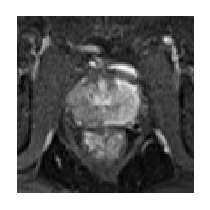
\includegraphics[width=1.5cm]{2_modality/figures/tikzimage/dce.eps}};
\begin{scope}[node distance=1.2cm]
\node[below of=t2w] (cap1) {\Large Fixed};
\end{scope}
\begin{scope}[node distance=6cm]
\node[below of=t2w] 	(dce) 			{\includegraphics[width=1.5cm]{2_modality/figures/tikzimage/t2.eps}};
\begin{scope}[node distance=1.2cm]
\node[below of=dce] (cap2) {\Large Moving};
\end{scope}
\end{scope}

\begin{scope}[node distance=5.5cm]
	\node[module,right of=t2w] (sim) {\Large Similarity \\ measure};
\end{scope}
\begin{scope}[node distance=3cm]
	\node[module,below of=sim] (int) {\Large Interpolator};
	\node[module,below of=int] (tra) {\Large Transform};
\end{scope}

\draw[line width=1mm,draw=blue!30,->] (t2w)--(sim);  
\draw[line width=1mm,draw=blue!30,->] (dce)--(tra); 

\begin{scope}[node distance=9cm]
	\node[module,right of=sim] (opt) {\Large Optimizer};
\end{scope}

\draw[draw=blue,->,line width=.5mm] (tra)--(int);
\draw[draw=blue,->,line width=.5mm] (int)--(sim);
\draw[draw=blue,->,line width=.5mm] (sim)--(opt) node[midway,above] {\Large Similarity} node[midway,below] {\Large metric};
\draw[draw=blue,->,line width=.5mm] (opt)|-(tra); 

\begin{pgfonlayer}{background}
	\path (sim.west |- sim.north)+(-0.5,.5) node (a) {};
    \path (opt.east |- tra.south)+(+0.5,-0.5) node (b) {};
          
    \path[fill=blue!10,rounded corners, draw=blue!20, dashed] (a) rectangle (b);
\end{pgfonlayer} 

\begin{scope}[node distance=5cm]
\node[right of=int] (arr) {
\begin{tikzpicture}
\arrows[1.9];
\end{tikzpicture}
};
\end{scope}
\end{tikzpicture}
\caption[Registration framework.]{Typical framework involved to solve the registration problem.}
\label{fig:frareg}
\end{figure}



%\tikzset{
%  ashadow/.style={opacity=.25, shadow xshift=0.07, shadow yshift=-0.07},
%}
%
%\def\arrows[#1]{         
%  \begin{scope}[scale=#1]
%	\node[align=center] at (0,0) {Loop \\ until \\ matching};  
%  
%    \draw[color=darkred, %
%    drop shadow={ashadow, color=red!60!black}] \arrow;
%
%    \draw[color=darkgreen, bottom color=green!60!black, top color=green!30, %
%    drop shadow={ashadow, color=green!60!black}] [rotate=120] \arrow;
%
%    \draw[color=darkblue, right color=blue!60, left color=blue!30, %
%    drop shadow={ashadow, color=blue!60!black}] [rotate=240] \arrow;
%
%    % to hide the green shadow
%    \draw[color=darkred, left color=red!60, right color=red!30] \arrow;
%  \end{scope}
%}
%
%\begin{tikzpicture}[node distance=3cm,thick,path image/.style={
%path picture={
%\node at (path picture bounding box.center) {
%\includegraphics[width=.5cm]{#1}
%};}}]
%\tikzstyle{conefill} = [path image=,fill opacity=0.8]
%
%\node[inner sep=0pt] (t2w) at (0,0)	{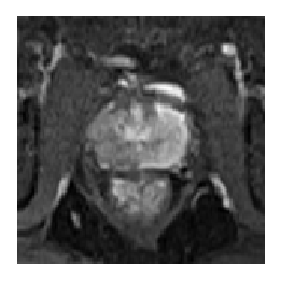
\includegraphics[width=1cm]{02_background/figures/tikzimage/dce.eps}};
%\begin{scope}[node distance=.8cm]
%\node[below of=t2w] (cap1) {Fixed};
%\end{scope}
%\begin{scope}[node distance=3.5cm]
%\node[below of=t2w] 	(dce) 			{\includegraphics[width=1cm]{02_background/figures/tikzimage/t2.eps}};
%\begin{scope}[node distance=.8cm]
%\node[below of=dce] (cap2) {Moving};
%\end{scope}
%\end{scope}
%
%\begin{scope}[node distance=2.5cm]
%	\node[module,right of=t2w] (sim) {Similarity \\ measure};
%\end{scope}
%\begin{scope}[node distance=1.75cm]
%	\node[module,below of=sim] (int) {Interpolator};
%	\node[module,below of=int] (tra) {Transform};
%\end{scope}
%\begin{scope}[node distance=5cm]
%	\node[module,right of=sim] (opt) {Optimizer};
%\end{scope}
%
%\draw[draw=blue,->,line width=.5mm] (tra)--(int);
%\draw[draw=blue,->,line width=.5mm] (int)--(sim);
%\draw[draw=blue,->,line width=.5mm] (sim)--(opt) node[midway,above] {Similarity} node[midway,below] {metric};
%\draw[draw=blue,->,line width=.5mm] (opt)|-(tra);
%
%\draw[line width=.8mm,draw=blue!30,->] (t2w)--(sim);  
%\draw[line width=.8mm,draw=blue!30,->] (dce)--(tra);  
%
%\begin{pgfonlayer}{background}
%	\path (sim.west |- sim.north)+(-0.3,.3) node (a) {};
%    \path (opt.east |- tra.south)+(+0.3,-0.3) node (b) {};
%          
%    \path[fill=blue!10,rounded corners, draw=blue!20, dashed] (a) rectangle (b);
%\end{pgfonlayer} 
%
%\begin{scope}[node distance=3cm]
%\node[right of=int] (arr) {
%\begin{tikzpicture}
%\arrows[1];
%\end{tikzpicture}
%};
%\end{scope}


Image registration plays a vital role in \ac{cad} systems using \ac{mpmri} images.
As it will be discussed in \acs{sec}\,\ref{sec:chp3:img-clas}, the features detected in each modality are grouped depending of their spatial location, requiring a perfect alignment of the \ac{mpmri} ahead of the classification.

Image registration is the procedure consisting of aligning an unregistered image --- also called moving image --- into a template image --- also called fixed image --- via a geometric transformation.
This problem is usually addressed as depicted in \ac{fig}\,\ref{fig:frareg}.
An iterative procedure takes place to infer the geometric transformation, parametric or non-parametric, via an optimizer which maximizes the similarity between the two images.
In the following, a review of the different components of a typical registration framework: transformation model, similarity metric, optimizer, and interpolation are presented.
To conclude a summary is given focusing on the registration approaches applied in \ac{cad} for \ac{cap} systems.
Exhaustive reviews covering all registration methods in computer science and medical fields can be found in~\cite{Maintz1998,Zitova2003}.

%From Sect. \ref{subsubsec:geotra} to \ref{subsubsec:int}, we individually review the different components of a typical registration framework (Fig \ref{fig:frareg}).
%Section \ref{subsubsec:regrev} will summarize the combinations of these components especially for the frameworks used in \ac{cad} systems. 

%% \setenumerate{listparindent=\parindent,itemsep=10px}
%% \setlist{noitemsep}
%% \begin{enumerate}[leftmargin=*]

%\item[$-$] \textbf{\textit{Geometric transformation models:}} 
\paragraph{Geometric transformation models}
%% From all \ac{cad} for \ac{cap} systems reviewed, only parametric transformation models have been used, mainly based on affine and elastic transformation.
%% Affine transformations provide dgrees of freedom managaing rotations and translation as with the rigid transformations but also shearing and scaling.
As previously mentioned, the registration process is equivalent to find a geometric transformation which minimizes the difference between two images.
From all \ac{cad} systems reviewed, only parametric methods have been implemented.
Three different groups of parametric transformation models have been used --- i.e., rigid, affine, and elastic --- each of them characterized by a specific degree of freedom.

The simplest transformation used in terms of degree of freedom is usually referred to as rigid transformation.
This type of transformation is only composed of a rotation and a translation.
Therefore, for the 2D case where $\mathbf{x} = (x,y) \in \mathbb{R}^2$, a rigid transformation $\mathcal{T}_R$ is formalized as:

\begin{eqnarray}
	\mathcal{T}_R(\mathbf{x}) & = & \begin{bmatrix}
		R & \mathbf{t} \\
		\mathbf{0^T} & 1
	\end{bmatrix} \mathbf{x} \ , \nonumber \\
	& = & \begin{bmatrix}
		\cos \theta & -\sin \theta & t_x \\
		\sin \theta & \cos \theta & t_y \\
		0 & 0 & 1
	\end{bmatrix}\begin{bmatrix}
		x \\
		y \\
		1
	\end{bmatrix} \ , \label{eq:rigtra} %\\
\end{eqnarray}

\noindent where $\theta$ is the rotation angle and $\{ t_x,t_y \}$ represents the translation along $\{x,y\}$ respectively.
In the case of 3D registration using volume, an additional component $z$ is introduced such that $\mathbf{x} = (x,y,z)$.
Thus, the rotation matrix $\mathbf{R}$ becomes of size $3 \times 3$ whereas the translation vector $\mathbf{t}$ consists of a vector of 3 variables. 
The geometric transformation $\mathcal{T}_R(\cdot)$ is embedded into a matrix of size $4 \times 4$.

The affine transformation provide additional degrees of freedom, providing rotation, translation, --- as with the rigid transformations --- and also shearing and scaling.
Hence, for a 2D space where $\mathbf{x} = (x,y) \in \mathbb{R}^2$, an affine transformation $\mathcal{T}_A$ is formalized as: 

\begin{eqnarray}
	\mathcal{T}_A(\mathbf{x}) & = & \begin{bmatrix}
		A & \mathbf{t} \\
		\mathbf{0^T} & 1
	\end{bmatrix} \mathbf{x} \ , \nonumber \\
	& = & \begin{bmatrix}
		a_{11} & a_{12} & t_x \\
		a_{21} & a_{22} & t_y \\
		0 & 0 & 1
	\end{bmatrix}\begin{bmatrix}
		x \\
		y \\
		1
	\end{bmatrix} \ . \label{eq:afftra}% 
\end{eqnarray}
\noindent where the 4 parameters $\{a_{11},a_{12},a_{21},a_{22}\}$ of the affine matrix and $\{ t_x, t_y \}$ of the translation encode the deformation.
As in the rigid registration case, in 3D the affine transformation $\mathcal{T}_A(\cdot)$ is of size $4 \times 4$ with 12 parameters involved.

Finally, the last group of transformation is known as elastic transformation and offers the advantage to handle local distortions.
In the reviewed \ac{cad} systems, the radial basis functions are used to formalize the local distortions such as:

\begin{equation}
	\mathcal{T}_E(\mathbf{x}) = \begin{matrix}
	a_{11} x - a_{12} y + t_x + \sum_i c_i g(\| \mathbf{x} - p_i \|) \\
	a_{21} x + a_{22} y + t_y + \sum_i c_i g(\| \mathbf{x} - p_i \|)
	\end{matrix} \ ,
\end{equation}

\noindent where $\mathbf{x}$ are the control points in both images and $g(\cdots)$ is the actual radial basis function. 

Two radial basis functions are used: (i) the \ac{tps} and (ii) the B-splines.
Apart from the formalism, these two approaches have a main difference: with B-splines, the control points are usually uniformly and densely placed on a grid whereas with \ac{tps}, the control points correspond to some detected or selected key points.
By using \ac{tps}, \citeauthor{Mitra2011} obtained more accurate and time efficient results than with the B-splines strategy~\cite{Mitra2012a}.

It is reasonable to point out that usually only rigid or affine registrations are used to register \ac{mpmri} from a same protocol.
Elastic registration methods are more commonly used to register multi-protocol images such as histopathology with \ac{mri} images~\cite{Toth2008,Toth2009}.

%\item[$-$] \textbf{\textit{Similarity measure:}} 
\paragraph{Similarity measure}
%% During the registration procedure, a similarity criterion is computed in order to evaluate the quality of the alignment performed.
%% Roughly speaking, this criterion will give the direction to take to the optimizer, in order to assign the most optimal values to the geometric transformation parameters.
The most naive similarity measure used in reviewed registration framework is the \acf{mse} of the \ac{si} of \ac{mri} images.
For a pair of images $I$ and $J$, the \ac{mse} is formalized as:

\begin{equation}
	\text{MSE} =\frac{1}{N} \sum_x \sum_y \left[ I(x,y) - J(x,y) \right]^2 \ ,
	\label{eq:mse}
\end{equation}
\noindent where $N$ is the total number of pixels.
This metric is not well suited when \ac{mpmri} images are involved due to the tissue appearance variations between the different modalities.

\begin{figure}
\centering
\hspace*{\fill}
\subfigure[Illustration of a joint histogram between to aligned image.]{\label{subfig:histoalgn}
\includegraphics[width=0.2\textwidth]{3_review/figures/processing/registration/histogram/jointhistoalg.eps}} \hfill
\subfigure[Illustration of a joint histogram between to misaligned image.]{\label{subfig:histomisalgn} 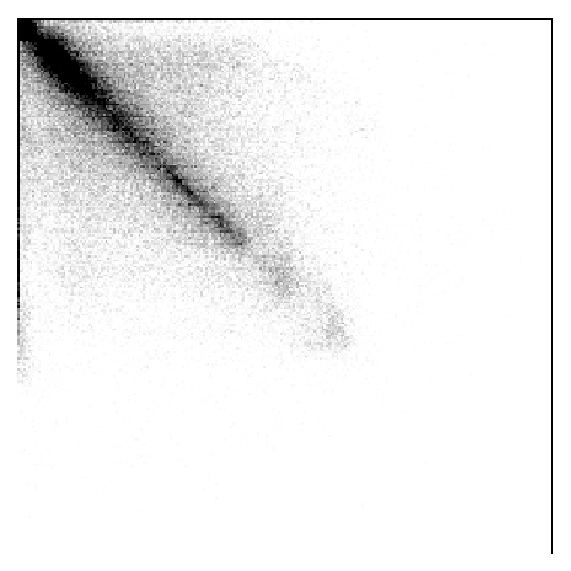
\includegraphics[width=0.2\textwidth]{3_review/figures/processing/registration/histogram/jointhistomisal.eps}}
\hspace*{\fill}
	\caption[Difference observed in joint histogram between aligned and misaligned images.]{Difference observed in joint histogram between aligned and misaligned images. The joint measure will be more concentrated of the histogram in the case that the images are aligned and more randomly distributed in the case that both images are more misaligned.}
        \label{fig:jointhisto}
\end{figure}

In this regard, \ac{mi} has been introduced as a similarity measure in registration framework in the late 1990's by \citeauthor{Pluim2003}.
The \ac{mi} measure finds its foundation in the assumption that a homogeneous region in the first modality image should also appear as a homogeneous region in the second modality, even if their \acp{si} are not identical.
Thus, those regions share information and the registration task is achieved by maximizing this common information.
Hence, \Ac{mi} of two images $A$ and $B$ is defined as:

\begin{equation}
	MI(A;B) = S(A) + S(B) - S(A,B) \ ,
	\label{eq:midef}
\end{equation}

\noindent where $S(A)$, $S(B)$, and $S(A,B)$ are the marginal entropies of $A$ and $B$ and the joint entropy, respectively.
Therefore, maximizing the \ac{mi} is the equivalent of minimizing the joint entropy. 
The joint entropy measure is related to the degree of uncertainty or dispersion of the data in the joint histogram of the images $A$ and $B$.
As shown in \acs{fig}\,\ref{fig:jointhisto}, the data in the joint histogram are concentrated in the case of aligned images (see \acs{fig}\,\ref{subfig:histoalgn}) while it is more randomly distributed in the case of misaligned images (see \acs{fig}\,\ref{subfig:histomisalgn}).
The entropy is computed based on an estimation of the \ac{pdf} of the images and thus histogram or Parzen window methods are a common way to estimate these \acp{pdf}.

A generalized form of \ac{mi}, \ac{cmi}, has been proposed by \citeauthor{Chappelow2011}.
\ac{cmi} encompasses interdependent information such as texture and gradient information into the metric.
Hence, for both of images $A$ and $B$, the image ensembles $\epsilon^{A}_n$ and $\epsilon^{B}_m$ are generated and composed of $n$ and $m$ images based on the texture and gradient.
Then, the \ac{cmi} is formulated such as:

\begin{equation}
	CMI(\epsilon^{A}_n;\epsilon^{B}_m) = S(\epsilon^{A}_n) + S(\epsilon^{B}_m) - S(\epsilon^{A}_n,\epsilon^{B}_m) \ .
	\label{eq:cmidef}
\end{equation}

From \acs{eq}\,\eqref{eq:cmidef}, note that \ac{cmi} is estimated from high-dimensional data and as a consequence the histogram-based methods to estimate the \acp{pdf} are not suitable anymore~\cite{Chappelow2011}. 
However, other alternative approaches are used such as the one employed in~\cite{Staring2009} to compute the $\alpha$-\ac{mi}~\cite{Hero2002}.
% which is based on the construction of entropic graphs which uses a \ac{knn} inside the high-dimensional feature space later used to estimate the \ac{mi}.

%\item[$-$] \textbf{\textit{Optimization methods:}} 
\paragraph{Optimization methods}
Registration is usually regarded as an optimization problem where the parameters of the geometric transformation model have to be inferred by minimizing/maximizing the similarity measure.
Iterative optimization methods are commonly used, where the most common methods used are the L-BFGS-B quasi-Newton method~\cite{Byrd1995} and the gradient descent~\cite{Viola1997}.
During our review, we noticed that authors do not usually linger over optimizer choice.

%\item[$-$] \textbf{\textit{Interpolation:}}
\paragraph{Interpolation} 
The registration procedure involves transforming an image and pixels mapped to non-integer points must be approximated using interpolation methods.
As for the optimization methods, we notice that little attention has been paid on the choice of those interpolations methods.
However, commonly used methods are bi-linear, nearest-neighbour, bi-cubic, spline, and inverse-distance weighting method~\cite{Mitra2012}.

%\item[$-$] \textbf{\textit{Registration methods used in \ac{cad} systems:}} 
\paragraph{Registration methods used in \ac{cad} systems}
\acs{tab}~\ref{tab:regtab} summarized the framework used to register \ac{mpmri} images in \ac{cad} for \ac{cap}.

\begin{table}
  \centering
  \caption[Classification of the different registration methods used in the \acs*{cad} systems reviewed.]{Classification of the different registration methods used in the \acs*{cad} systems reviewed. Acronyms: mean squared error (MSE), mutual information (MI), combined mutual information (CMI), gradient descent (GD), limited-memory Broyden-Fletcher-Goldfarb-Shannon box constraints (L-BFGS-B).}
  \scriptsize
    \begin{threeparttable}
      \begin{tabular}{l l c c c c c c c c}\hline
        \toprule
        \textbf{Study} & \textbf{Modality} & \multirow{2}{*}{\textbf{Type}} & \multicolumn{2}{c}{\textbf{Geometric model}} & \multicolumn{3}{c}{\textbf{Similarity measure}} & \multicolumn{2}{c}{\textbf{Optimizer}} \\
        \cmidrule{4-10}
        \textbf{index} & \textbf{registered} & & Affine & Elastic & \acs{mse} & \acs{mi} & \acs{cmi} & GD & L-BFGS-B \\
        \midrule
        \cite{Ampeliotis2007,Ampeliotis2008} & \ac{t2w} - \ac{dce} & 2D & \cmark & $-$ & \cmark & $-$ & $-$ & $-$ & $-$ \\
        \cite{Giannini2013,giannini2015fully} & \ac{t2w} - \ac{dw} & 2D & \cmark & \cmark & $-$ & $-$ & $-$ & $-$ & $-$  \\
        \cite{Giannini2013,giannini2015fully} & \ac{t2w} - \ac{dce} & 2D & \cmark & \cmark & $-$ & \cmark & $-$ & \cmark & $-$ \\
        \cite{Viswanath2008a,Viswanath2009} & \ac{t2w} - \ac{dce} & 2D & \cmark & $-$ & $-$ & \cmark & $-$ & $-$ & $-$ \\
        \cite{Viswanath2011} & \ac{t2w} - \ac{dce} - \ac{dw} & 3D & \cmark & $-$ & $-$ & $-$ & \cmark & \cmark & $-$  \\
        \cite{Vos2008} & \ac{t2w} - \ac{dce} & 3D & \cmark & $-$ & $-$ & \cmark & $-$ & $-$ & $-$ \\
        \cite{Vos2010} & \ac{t2w} - \ac{dce} & 3D & \cmark & \cmark & $-$ & \cmark & $-$ & $-$ & \cmark \\
        \bottomrule
      \end{tabular}
      \begin{tablenotes}
        \footnotesize
      \item Notes:
      \item {$-$}: not used or not mentioned.
      \item {\cmark}: used or implemented.
      \end{tablenotes}
    \end{threeparttable}
\label{tab:regtab}  
\end{table}

\citeauthor{Ampeliotis2008} in~\cite{Ampeliotis2007,Ampeliotis2008} did not use the framework as presented in \acs{fig}\,\ref{fig:frareg} to register 2D \ac{t2w}-\ac{mri} and \ac{dce}-\ac{mri} images.
By using image symmetries and the \ac{mse} metric, they found the parameters of an affine transformation but without using a common objective function.
The scale factor, the rotation, and the translation are independently and sequentially estimated.

\cite{Giannini2013} used also a in-house registration method for 2D \ac{t2w}-\ac{mri} and \ac{dw}-\ac{mri} images using an affine model~\cite{Giannini2013,giannini2015fully}.
The bladder is first segmented in both modalities in order to obtain its contours and to focus on the registration and minimize the distance between the contours.

\citeauthor{Giannini2013} and also \citeauthor{Vos2010} used a framework based on finding an affine transformation to register the \ac{t2w}-\ac{mri} and \ac{dce}-\ac{mri} images using \ac{mi}~\cite{Rueckert1999,Giannini2013,Vos2010}.
Then, an elastic registration using B-spline takes place using the affine parameters to initialize the geometric model with the same similarity measure.
However, the two approaches differ regarding the choice of the optimizer since a gradient descent is used in~\cite{Giannini2013} and a quasi-Newton method in~\cite{Vos2010}.
Moreover, \citeauthor{Giannini2013} applied a 2D registration whereas \citeauthor{Vos2010} registered 3D volumes.

\citeauthor{Viswanath2008a} as well as \citeauthor{Vos2008} registered \ac{t2w}-\ac{mri} and \ac{dce}-\ac{mri} images using an affine registration and a \ac{mi} metric~\cite{Viswanath2008a,Viswanath2009,Vos2008}.
However, the choice of the optimizer has not been specified. 
Furthermore, \citeauthor{Viswanath2008a} focused on 2D registration~\cite{Viswanath2008a,Viswanath2009} while \citeauthor{Vos2008} performed 3D registration~\cite{Vos2008}.

Finally, \citeauthor{Viswanath2011} performed a 3D registration with the three modalities, \ac{t2w}-\ac{mri}, \ac{dce}-\ac{mri}, and \ac{dw}-\ac{mri}, using an affine transformation model combined with the \ac{cmi} similarity measure~\cite{Viswanath2011}.
Moreover, in this latter work, the authors employed a gradient descent approach~\cite{Chappelow2011} to solve this problem but suggested that the Nelder-Mead simplex and the quasi-Newton methods are other possible solutions.

%\end{enumerate}

\section{Image classification framework}\label{sec:chp3:img-clas}


\subsection{\acs*{cade}: \acsp*{roi} detection/selection} \label{subsec:chp3:img-clas:roiSel}

\begin{table}
  \caption{Overview of the \acs*{cade} strategies employed in \acs*{cad} systems.}
  \scriptsize
  \centering
  \begin{tabularx}{\textwidth}{l >{\raggedleft\arraybackslash}X}
    \toprule
    \textbf{\ac{cade}: \acp{roi} selection strategy} & \textbf{References} \\
    \midrule
    All voxels-based approach & \cite{Artan2009,Artan2010,Giannini2013,Kelm2007,Liu2009,Lopes2011,Matulewicz2013,Mazzetti2011,Ozer2009,Ozer2010,Parfait2012,Sung2011,Tiwari2007,Tiwari2008,Tiwari2009,Tiwari2009a,Tiwari2010,Tiwari2012,Tiwari2013,Viswanath2008,Viswanath2008a,Viswanath2009,Viswanath2011,Viswanath2012,trigui2016classification,trigui2017automatic,lehaire2014computer,khalvati2015automated,rampun2015classifying,rampun2015computer,rampun2016computer,rampun2016computerb,rampun2016quantitative} \\
    Lesions candidate detection & \cite{Litjens2011,Litjens2012,Litjens2014,Vos2012,cameron2014multiparametric,cameron2016maps} \\
    \bottomrule
  \end{tabularx}
\label{tab:cade}
\end{table}

As discussed in the introduction and shown in \acs{fig}\,\ref{fig:wkfcad}, the image classification framework is often composed of a \ac{cade} and a \ac{cadx}.
In this section, we focus on studies which embed a \ac{cade} in their framework.
Two approaches are considered to define a \ac{cade}: (i) voxel-based delineation and (ii) lesion segmentation.
These methods are summarized in \acs{tab}~\ref{tab:cade}.
The first strategy is in fact linked to the nature of the classification framework and concerns the majority of the studies reviewed~\cite{Artan2009,Artan2010,Giannini2013,Kelm2007,Liu2009,Lopes2011,Matulewicz2013,Mazzetti2011,Ozer2009,Ozer2010,Parfait2012,Sung2011,Tiwari2007,Tiwari2008,Tiwari2009,Tiwari2009a,Tiwari2010,Tiwari2012,Tiwari2013,Viswanath2008,Viswanath2008a,Viswanath2009,Viswanath2011,Viswanath2012,trigui2016classification,trigui2017automatic,lehaire2014computer,khalvati2015automated,rampun2015classifying,rampun2015computer,rampun2016computer,rampun2016computerb,rampun2016quantitative}.
Each voxel is a possible candidate and will be classified as cancer or healthy.
The second group of methods is composed of method implementing a lesion segmentation algorithm to delineate potential candidates to further obtain a diagnosis through the \ac{cadx}.
This approach is borrowed from other application areas such as breast cancer.
These methods are in fact very similar to the classification framework used in \ac{cadx} later.

\citeauthor{Vos2012} highlighted lesion candidates by detecting blobs in the \ac{adc} map~\cite{Vos2012}.
These candidates are filtered using some \textit{a priori} criteria such as \ac{si} or diameter.
As mentioned in \acs{sec}\,\ref{subsec:chp2:imaging:mrsi} and \acs{tab}~\ref{tab:modmri}, low \ac{si} in \ac{adc} map can be linked to potential \ac{cap}.
Hence, blob detectors are suitable to highlight these regions. 
Blobs are detected in a multi-resolution scheme, by computing the three main eigenvalues $\{ \lambda_{\sigma,1},\lambda_{\sigma,2},\lambda_{\sigma,3} \}$ of the Hessian matrix, for each voxel location of the \ac{adc} map at a specific scale $\sigma$~\cite{Li2003}.
The probability $p$ of a voxel $\mathbf{x}$ being a part of a blob at the scale $\sigma$ is given by:

\begin{equation}
P(\mathbf{x},\sigma) = \begin{cases}
	\frac{\| \lambda_{\sigma,3}(\mathbf{x}) \|^{2}}{\| \lambda_{\sigma,1} (\mathbf{x}) \|} \ , & \text{if } \lambda_{\sigma,k}(\mathbf{x}) > 0 \text{ with } k = \{1,2,3\} \  , \\
	0 \ , & \text{otherwise} \ .
\end{cases}
\label{eq:blobdet}
\end{equation}

\noindent The fusion of the different scales is computed as:

\begin{equation}
	L(\mathbf{x}) = \max P(\mathbf{x},\sigma) , \forall \sigma \ .
	\label{eq:fusionBlob}
\end{equation}

The candidate blobs detected are then filtered depending on their appearances --- i.e., maximum of the likelihood of the region, diameter of the lesion --- and their \ac{si} in \ac{adc} and \ac{t2w}-\ac{mri} images.
The detected regions are then used as inputs for the \ac{cadx}.
\citeauthor{cameron2016maps} used a similar approach by automatically selecting low \ac{si} connected regions in the \ac{adc} map with a size larger than \SI{1}{\milli\metre\squared}~\cite{cameron2014multiparametric,cameron2016maps}.

\citeauthor{Litjens2011} used a pattern recognition approach in order to delineate the \acp{roi}~\cite{Litjens2011}.
A blobness map is computed in the same manner as in~\cite{Vos2010} using the multi-resolution Hessian blob detector on the \ac{adc} map, \ac{t2w}, and pharmacokinetic parameters maps (see \acs{sec}\,\ref{subsec:chp3:img-clas:CADX-fea-dec} for details about those parameters).
Additionally, the position of the voxel $\mathbf{x}=\{x,y,z\}$ is used as a feature as well as the Euclidean distance of the voxel to the prostate center.
Hence, each feature vector is composed of 8 features and a \ac{svm} classifier is trained using a \ac{rbf} kernel (see \acs{sec}\,\ref{subsec:chp3:img-clas:CADX-clas} for more details).

Subsequently, \citeauthor{Litjens2012} modified this approach by including only features related to the blob detection on the different maps as well as the original \acp{si} of the parametric images~\cite{Litjens2012}.
Two new maps are introduced based on texture and a \ac{knn} classifier is used instead of a \ac{svm} classifier
The candidate regions are then extracted by performing a local maxima detection followed by post-processing region-growing and morphological operations. 

\subsection{\acs*{cadx}: Feature detection} \label{subsec:chp3:img-clas:CADX-fea-dec}

Discriminative features which help to recognize \ac{cap} from healthy tissue need to be first detected.
This processing is known in computer vision as feature extraction. 
However, feature extraction also refer to the name given in pattern recognition to some types of dimension reduction methods which are later presented.
In order to avoid confusion between these two aspects, in this survey, the procedure ``detecting'' or ``extracting'' features from images and signals is defined as feature detection.
This section summarizes the different features used in \ac{cad} for \ac{cap} and are summarized in \acs{tab}~\ref{tab:feat}.  

%%%% THIS TABLE NEEDS TO BE CHANG
\newgeometry{margin=1cm}
\thispagestyle{empty}
\begin{table}
  \centering
  \caption{Overview of the feature detection methods used in \ac{cad} systems.}\label{tab:feat}
  \footnotesize
  \begin{threeparttable}
    \renewcommand{\arraystretch}{.7}
    \begin{tabular}{p{.5\linewidth} p{.4\linewidth}}
      \hline \\ [-1.5ex]
      \textbf{Feature detection methods} & \textbf{Indexes} \\ \\ [-1.5ex]
      \hline \\ [-1.5ex]
      \textbf{\ac{mri} image:} & \\ \\ [-1.5ex]
      \quad \textit{Voxel-wise detection} &  \\ \\ [-1.5ex]
      \quad \quad Intensity-based & $^{\text{{\cmarksmall}- -}}$\cite{Ampeliotis2007,Ampeliotis2008,Vos2008}\par $^{\text{- - {\cmarksmall}}}$\cite{Giannini2013}\par $^{\text{{\cmarksmall}- {\cmarksmall}}}$\cite{Artan2009,Artan2010,Chan2003,Langer2009,Litjens2011,Litjens2012,Litjens2014,Liu2009,Ozer2009,Ozer2010}\par $^{\text{{\cmarksmall}{\cmarksmall}{\cmarksmall}}}$\cite{Niaf2011,Niaf2012} \\ 
      \quad \quad Edge-based & \\
      \quad \quad \quad Prewitt operator & $^{\text{{\cmarksmall}- -}}$\cite{Tiwari2009a,Tiwari2010,Tiwari2013,Viswanath2008} \\
      \quad \quad \quad Sobel operator & $^{\text{{\cmarksmall}- -}}$\cite{Tiwari2009a,Tiwari2010,Tiwari2013,Viswanath2008,Viswanath2009,Viswanath2011,Viswanath2012}\par $^{\text{{\cmarksmall}{\cmarksmall}{\cmarksmall}}}$\cite{Niaf2011,Niaf2012} \\
      \quad \quad \quad Kirsch operator & $^{\text{{\cmarksmall}- -}}$\cite{Tiwari2009a,Tiwari2010,Tiwari2013,Viswanath2008,Viswanath2009,Viswanath2011,Viswanath2012}\par $^{\text{{\cmarksmall}{\cmarksmall}{\cmarksmall}}}$\cite{Niaf2011,Niaf2012} \\
      \quad \quad \quad Gabor filtering & $^{\text{{\cmarksmall}- -}}$\cite{Tiwari2012,Viswanath2008,Viswanath2012} \\ 
      \quad \quad Texture-based & \\
      \quad \quad \quad Haralick features & $^{\text{{\cmarksmall}- -}}$\cite{Antic2013,Tiwari2009a,Tiwari2010,Tiwari2013,Viswanath2008,Viswanath2009,Viswanath2012}\par $^{\text{{\cmarksmall}{\cmarksmall}-}}$\cite{Viswanath2011}\par $^{\text{{\cmarksmall}{\cmarksmall}{\cmarksmall}}}$\cite{Litjens2012,Niaf2011,Niaf2012} \\
      \quad \quad \quad Fractal analysis & $^{\text{{\cmarksmall}- -}}$\cite{Lopes2011,Lv2009} \\
      \quad \quad \quad \Ac{dct} & $^{\text{{\cmarksmall}{\cmarksmall}{\cmarksmall}}}$\cite{Chan2003} \\
      \quad \quad \quad Wavelet-based features & $^{\text{{\cmarksmall}- -}}$\cite{Viswanath2012} \\
      \quad \quad \quad Gaussian filter bank & $^{\text{{\cmarksmall}- -}}$\cite{Litjens2014} \\ 
      \quad \quad Position-based & \cite{Chan2003,Litjens2011,Litjens2012,Litjens2014} \\ \\ [-1.5ex]
      \quad \textit{Region-wise detection} &  \\ \\ [-1.5ex]
      \quad \quad Statistical-based & \\
      \quad \quad \quad Percentiles & $^{\text{- {\cmarksmall}-}}$\cite{Vos2008a} \par $^{\text{- - {\cmarksmall}}}$\cite{Antic2013,Peng2013}\par $^{\text{{\cmarksmall}{\cmarksmall}-}}$\cite{Vos2010}\par $^{\text{{\cmarksmall}{\cmarksmall}{\cmarksmall}}}$\cite{Litjens2011,Litjens2012,Litjens2014,Niaf2011,Niaf2012,Vos2012} \\
      \quad \quad \quad Statistical-moments & $^{\text{{\cmarksmall}- -}}$\cite{Ampeliotis2007,Ampeliotis2008,Tiwari2009a,Tiwari2010,Tiwari2013,Viswanath2008,Viswanath2009,Viswanath2012}\par $^{\text{- - {\cmarksmall}}}$\cite{Antic2013}\par $^{\text{{\cmarksmall}{\cmarksmall}-}}$\cite{Viswanath2011}\par $^{\text{{\cmarksmall}- {\cmarksmall}}}$\cite{Peng2013}\par $^{\text{{\cmarksmall}{\cmarksmall}{\cmarksmall}}}$\cite{Litjens2011,Litjens2012,Litjens2014,Niaf2011,Niaf2012} \\
      \quad \quad Histogram-based & \\
      \quad \quad \quad \acs{pdf} & $^{\text{{\cmarksmall}{\cmarksmall}{\cmarksmall}}}$\cite{Liu2013} \\
      \quad \quad \quad \acs{hog} & $^{\text{{\cmarksmall}{\cmarksmall}{\cmarksmall}}}$\cite{Liu2013} \\
      \quad \quad \quad Shape context & $^{\text{{\cmarksmall}{\cmarksmall}{\cmarksmall}}}$\cite{Liu2013} \\
      \quad \quad \quad \acs{lbp} & $^{\text{{\cmarksmall}{\cmarksmall}{\cmarksmall}}}$\cite{Liu2013} \\
      \quad \quad Anatomical-based & \cite{Litjens2012,Litjens2014,Matulewicz2013} \\ \\ [-1.5ex]
      \textbf{\ac{dce} signal:} & \\ \\ [-1.5ex]
      \quad Whole spectra approach & \cite{Ampeliotis2007,Ampeliotis2008} \\
      \quad Semi-quantitative approach & $^{\text{{\mmarksmall}}}$\cite{Puech2009}\par \cite{Mazzetti2011,Niaf2011,Niaf2012,Sung2011} \\
      \quad Quantitative approach &  \\
      \quad \quad Toft model & $^{\text{{\mmarksmall}}}$\cite{Liu2013,Peng2009}\par \cite{Giannini2013,Langer2009,Litjens2011,Litjens2012,Litjens2014,Mazzetti2011,Niaf2011,Niaf2012} \\
      \quad \quad Brix model & $^{\text{{\mmarksmall}}}$\cite{Artan2009,Artan2010,Ozer2009,Ozer2010}\par \cite{Liu2009,Sung2011} \\
      \quad \quad Weibull function & \cite{Giannini2013,Mazzetti2011} \\
      \quad \quad PUM & \cite{Giannini2013,Mazzetti2011} \\
      \\ [-1.5ex]
      \textbf{\ac{mrsi} signal:} & \\ \\ [-1.5ex]
      \quad Whole spectra approach & \cite{Kelm2007,Matulewicz2013,Parfait2012,Tiwari2007,Tiwari2008,Tiwari2009,Tiwari2009a,Tiwari2010,Tiwari2013,Viswanath2008} \\
      \quad Quantification approach & \cite{Kelm2007,Parfait2012} \\
      \quad Wavelet-based approach & \cite{Tiwari2012} \\ \\ [-1.5ex]
      \hline
    \end{tabular}
    \begin{tablenotes}
      \footnotesize
    \item Notes:
    \item ( {\cmarksmall}$|$- {\cmarksmall}$|$- {\cmarksmall}$|$- ): triplet stating the implementation or not of the feature for respectively \ac{t2w}-\ac{mri} images, \ac{dce}-\ac{mri} images, \ac{dw}-\ac{mri} images.
    \item {\cmarksmall}: used or implemented.
    \item {\mmarksmall}: partially implemented.
    \end{tablenotes}
  \end{threeparttable}
\end{table}
\restoregeometry



\subsubsection{Image-based features}\label{subsubsec:chp3:img-clas:CADX-fea-dec:Img-fea}

This section focuses on image-based features which can be categorized into two categories: (i) voxel-wise detection and (ii) region-wise detection.

\paragraph{Voxel-wise detection}
This strategy refers to the fact that a feature is extracted at each voxel location.
As discussed in \acs{sec}\,\ref{sec:chp2:imaging}, \ac{cap} has an influence on the \ac{si} in \ac{mpmri} images.
Therefore, intensity-based feature is the most commonly used feature~\cite{Ampeliotis2007,Ampeliotis2008,Vos2008,rampun2016computerb,rampun2015classifying,Giannini2013,Artan2009,Artan2010,Chan2003,Langer2009,Litjens2011,Litjens2012,Litjens2014,Liu2009,Ozer2009,Ozer2010,trigui2016classification,trigui2017automatic,cameron2014multiparametric,cameron2016maps,khalvati2015automated,chung2015prostate,giannini2015fully,Niaf2011,Niaf2012,lehaire2014computer}.
This feature consists in the extraction of the intensity of the \ac{mri} modality of interest.

Edge-based features have also been used to detect \ac{si} changes but bring additional information regarding the the \ac{si} transition.
Each feature is computed by convolving the original image with an edge operator.
Three operators are commonly used: (i) Prewitt operator~\cite{Prewitt1970}, (ii) Sobel operator~\cite{Sobel1970}, and (iii) Kirsch operator~\cite{Kirsch1971}.
These operators differ due to the kernel used which attenuate more or less the noise.
Multiple studies used the resulting magnitude and orientation of the edges computed in their classification frameworks~\cite{Niaf2011,Niaf2012,Tiwari2009a,Tiwari2010,Tiwari2013,Viswanath2008,Viswanath2011,rampun2016quantitative,rampun2015computer,rampun2016computer,lehaire2014computer,khalvati2015automated,chung2015prostate}.

\begin{figure}
	\hspace*{\fill}
		\subfigure[$\theta=0^{\circ}$.]{\label{subfig:gab1} 
\includegraphics[width=0.2\linewidth]{3_review/figures/feature-detection/gabor/gabor_1.eps}} \hfill
		\subfigure[$\theta=60^{\circ}$.]{\label{subfig:gab2} 
\includegraphics[width=0.2\linewidth]{3_review/figures/feature-detection/gabor/gabor_2.eps}} \hfill
		\subfigure[$\theta=120^{\circ}$.]{\label{subfig:gab3} 
\includegraphics[width=0.2\linewidth]{3_review/figures/feature-detection/gabor/gabor_3.eps}} \hfill
		\subfigure[$\theta=180^{\circ}$.]{\label{subfig:gab4} 
\includegraphics[width=0.2\linewidth]{3_review/figures/feature-detection/gabor/gabor_4.eps}}
	\hspace*{\fill}
	\caption[Illustration of 4 different Gabor filters.]{Illustration of 4 different Gabor filters varying their orientations $\theta$.}
	\label{fig:gabor}
\end{figure}

Gabor filter~\cite{Gabor1946,Daugman1985} offer an alternative to the usual edge detector, with the possibility to tune the direction and the frequency of the filter to encode a specific pattern. 
A Gabor filter is defined by the modulation of a Gaussian function with a sine wave which can be further rotated and is formalized as in \acs{eq}\,\ref{eq:gabor}.
\begin{equation}
	g(x,y;\theta,\psi,\sigma,\gamma) = \exp \left( - \frac{x'^{2}+ \gamma^{2}y'^{2}}{2 \sigma^{2}} \right) \cos \left( 2 \pi \frac{x'}{\lambda} + \phi \right) \ ,
        \label{eq:gabor}
\end{equation}

\noindent with 

\begin{eqnarray}
	x' & = & s\left( x \cos \theta + y \sin \theta \right) \ , \nonumber \\
	y' & = & s \left( - x \sin \theta + y \cos \theta \right) \ , \nonumber
\end{eqnarray}

\noindent where $\lambda$ is the wavelength of the sinusoidal factor, $\theta$ represents the orientation of the Gabor filter, $\psi$ is the phase offset, $\sigma$ is the standard deviation of the Gaussian envelope, $\gamma$ is the spatial aspect ratio, and $s$ is the scale factor.
In an effort to characterize pattern and texture, a bank of Gabor filters is usually created with different angles, scale, and frequency --- refer to \acs{fig}\,\ref{fig:gabor} --- and then convolved with the image.
\citeauthor{Viswanath2012}, \citeauthor{Tiwari2012} and more recently \citeauthor{khalvati2015automated} and \citeauthor{chung2015prostate} have designed a bank of Gabor filters to characterized texture and edge information in \ac{t2w}-\ac{mri} and \ac{dw}-\ac{mri} modalities.

%%%% GO here 
\citeauthor{rampun2016computer} employed rotationally invariant Gabor filter banks ( \ac{lm}~\cite{varma2005statistical}) which takes edges and sopts/bars into account. 
The \ac{lm} consists of 48 filters including first and second derivatives of Gaussian at 6 orientations and 3 scales (36 filters), in addition to 8 Laplacian of Gaussian and 4 Gaussians filters.
The scale of proposed filters vary between $\sigma = 1$ to $\sigma = 10$ \si{\px}


Texture-based features provide other characteristics discerning \ac{cap} from healthy tissue.
The most common texture analysis for image classification is based on the \ac{glcm} with their related statistics which have been proposed by \citeauthor{Haralick1973} in~\cite{Haralick1973}.
In a neighborhood around a central voxel, a \ac{glcm} is build considering each voxel pair defined by a specific distance and angle.
Then, using the \ac{glcm}, a set of statistical features is computed as defined in \acs{tab}~\ref{tab:glcm} and assigned to the location of the central voxel.
Therefore, $N$ --- up to 14 --- statistical maps are derived from the \ac{glcm} analysis, one per statistics presented in \acs{tab}~\ref{tab:glcm}.
\ac{glcm} is commonly used in \ac{cad} systems, on the different \ac{mri} modalities, namely \ac{t2w}-\ac{mri}, \ac{dce}-\ac{mri}, or \ac{dw}-\ac{mri}~\cite{Antic2013,Niaf2011,Niaf2012,Tiwari2009a,Tiwari2010,Tiwari2013,Viswanath2008,Viswanath2009,Viswanath2011,Viswanath2012,trigui2016classification,rampun2015computer,rampun2016computer,rampun2016quantitative,cameron2014multiparametric,cameron2016maps,khalvati2015automated,chung2015prostate,lehaire2014computer}.
However, the statistics extracted from the \ac{glcm} across studies vary.

\begin{table}
  \caption[The 14 statistical features used in conjunction with \acs*{glcm} analysis.]{The 14 statistical features for texture analysis commonly computed from the \acs*{glcm} $p$ as presented by~\cite{Haralick1973}.}
  \scriptsize
  \renewcommand{\arraystretch}{1.5}
  \centering
  \begin{tabular}{ll}
    \toprule
    \textbf{Statistical features} & \textbf{Formula} \\
    \midrule
    Angular second moment & $\sum_i \sum_j p(i,j)^2 $  \\
    Contrast & $\sum_{n=0}^{N_g - 1} n^2 \left[ \sum_{i=1}^{N_g - 1} \sum_{j=1}^{N_g - 1} p(i,j) \right] \ , | i-j |=n  $ \\
    Correlation & $\frac{\sum_i \sum_j (ij) p(i,j) - \mu_x \mu_y}{\sigma_x \sigma_y}  $ \\
    Variance & $\sum_i \sum_j (i - \mu)^2 p(i,j)  $ \\
    Inverse difference moment & $\sum_i \sum_j \frac{1}{1+(i - \mu)^2} p(i,j)  $ \\
    Sum average & $\sum_{i=2}^{2N_g} i p_{x+y}(i)  $ \\
    Sum variance & $\sum_{i=2}^{2N_g} (i-f_s)^2 p_{x+y}(i)  $ \\
    Sum entropy & $ - \sum_{i=2}^{2N_g} p_{x+y}(i) \log p_{x+y}(i)  $ \\
    Entropy & $ - \sum_i \sum_j p(i,j) \log p(i,j) $ \\
    Difference variance & $\sum_{i=0}^{N_g-1} i^2 p_{x-y}(i)  $ \\
    Difference entropy & $ - \sum_{i=0}^{N_g-1} p_{x-y}(i) \log p_{x-y}(i)  $ \\
    Info. measure of corr. 1 & $\frac{S(X;Y)-S_1(X;Y)}{\max(S(X),S(Y))}  $ \\
    Info. measure of corr. 2 & $\sqrt{\left( 1 - \exp \left[ -2( H_2(X;Y) - H(X;Y) ) \right] \right)}  $ \\
    Max. corr. coeff. & $ \sqrt{\lambda_2} \ , \text{of } Q(i,j) = \sum_k \frac{p(i,k)p(j,k)}{p_x(i)p_y(k)}  $ \\
    \bottomrule
  \end{tabular}
  \label{tab:glcm}
\end{table}

Fractal analysis and more precisely a local estimation of the fractal dimension \cite{Benassi1998} describing the texture roughness at a specific location was used in \cite{Lopes2011}.
A wavelet-based method in a multi-resolution framework was used to estimate the fractal dimension.
Cancerous tissue were characterized to have a higher fractal dimension than healthy tissue.

Chan \textit{et al.}~\cite{Chan2003} described the texture using the frequency signature via the \acf{dct} \cite{Ahmed1974}) defining a neighbourhood of $7 \times 7$ pixels for each of the modalities that they used.
The \ac{dct} allows to decompose a portion of image into a coefficients space where few of these coefficients encoded the visually significant information.
The \ac{dct} coefficients are computed such as:

\begin{equation}
	C_{k_1,k_2} = \sum_{m=0}^{M-1} \sum_{n=0}^{N-1} p_{m,n} \cos \left[ \frac{\pi}{M} \left( m + \frac{1}{2} \right) k_1 \right] \cos \left[ \frac{\pi}{N} \left( n + \frac{1}{2} \right) k_2 \right] \ ,
\end{equation}

\noindent where $C_{k_1,k_2}$ is the \ac{dct} coefficient at the position $k_1,k_2$, $M$ and $N$ are the dimension of the neighbourhood and $p_m,n$ is the pixel \ac{si} at the position $p_{m,n}$.

Viswanath \textit{et al.}~\cite{Viswanath2012} projected \ac{t2w} images into the wavelet space, using Haar wavelet, and used the coefficients obtained from the decomposition as features.
%The wavelet family used for the decomposition was the Haar wavelet.

Finally Litjens \textit{et al.} in \cite{Litjens2011} computed the texture map based on \ac{t2w} images using a Gaussian filer bank.
%% Euclidean distance from each voxel to the prostate center as well as the individual distance in the three directions $x$, $y$ and $z$. \cite{Chan2003} embedded the same information but this time using cylindrical coordinate $r$, $\theta$ and $z$ corresponding to the radius, azimuth and elevation respectively.


\paragraph{Region-wise detection}

Unlike the previous section, another strategy is to study an entire region and extract characteristic features corresponding to this region.
The most common approach reviewed can be classified as statical methods.
First a feature map is computed for the whole image instaed of using single voxels.
Then, \acp{roi} are defined and statistics are extracted from each of these regions.
The most widely used statistics is based on percentiles and is widely used \cite{Antic2013,Litjens2011,Litjens2012,Litjense2014,Peng2013,Tiwari2009a,Tiwari2010,Tiwari2013,Viswanath2008,Viswanath2008a,Viswanath2011,Viswanath2012,Vos2008,Vos2008a,Vos2010,Vos2012}.
The percentile used is usually manually determined observing the distribution and corresponds to the best discriminant value differentiating malignant and healthy tissue.
In addition, statistic-moments such as mean, standard deviation, kurtosis and skewness are also used \cite{Ampeliotis2007,Ampeliotis2008,Antic2013,Niaf2011,Niaf2012,Peng2013}.
Litjense \textit{et al.} in \cite{Litjense2014} also introduced a feature based on symmetry.
They compute the mean of a candidate lesion as well as its mirrored counter-part and compute the quotient as feature.

Another subset of features are anatomic which were also used in \cite{Litjens2012,Litjense2014,Matulewicz2013}. 
Litjense \textit{et al.} in \cite{Litjense2012, Litjense2014} computed the volume, compactness and sphericity related to the region to integrate it in their feature vector.
Matulewicz \textit{et al.}~\cite{Matulewicz2013} introduced four features corresponding to the percentage of tissue belonging to the regions\ac{pz}, \ac{cg}, periurethral region or outside prostate region for the considered \ac{roi}.

In contrast to anatomical are histogram-based features.
For instance, Liu \textit{et al.}~\cite{Liu2013} introduced four different types of histogram-based features.
The first type corresponds to the histogram of the \ac{si} of the image.
The second type is the \acf{hog} \cite{Dalal2005}.
\Ac{hog} descriptor describes the local shape of the object of interest by using distribution of gradient directions.
This descriptor is extracted mainly in three steps.
First the gradient image and its corresponding magnitude and direction are computed.
Then, the \ac{roi} is divided into cells and an oriented-based histogram is generated for each cell.
At each pixel location, the orientation of the gradient will vote for a bin of the histogram and this vote is weighted by the magnitude of the same gradient.
Finally, The cells are grouped into block and each block is normalized.
The third histogram-based type used in \cite{Liu2013} was shape context \cite{Belongie2002}.
The shape context is also a way to describe the shape of an object of interest.
First, a set of points defining edges have to be detected and for each point of each edge, a log-polar-based histogram is computed using the relative points distribution.
The last set of histogram-based feature extracted is based on the framework described in \cite{Zhao2012} which is using the Fourier transform of the histogram created via \acf{lbp} \cite{Ojala1996}.
\Ac{lbp} is generated by comparing the value of the central pixel with its 8-connected neighbours.
Then, in the \ac{roi}, the histogram of the \ac{lbp} distribution is computed.
The \acf{dft} of the \ac{lbp} histogram is used to make the feature invariant to rotation.

The last group of region-based feature is based on fractal analysis.
The features proposed are based on estimating the fractal dimension which is a statistical index representing the complexity of what is analysed.
Lv \textit{et al,}~\cite{Lv2009} proposed two features based on fractal dimension: (i) texture fractal dimension and (ii) histogram fractal dimension.
The first feature is based on estimating the fractal dimension on the \ac{si} of each image.
Hence, this feature is a statistical characteristic of the image roughness.
The second fractal dimension is estimated in the \ac{pdf} of each image and characterises the complexity of the \ac{pdf}.
Lopes \textit{et al.}~\cite{Lopes2011} proposed a 3D version to estimate the fractal dimension of a volume using wavelet decomposition.


\subsubsection{\Ac{dce}-based features}\label{subsubsec:chp3:img-clas:CADX-fea-dec:DCE-fea}

\ac{dce}-\ac{mri} is more commonly based on a \ac{si} analysis over time as presented in Sect.~\ref{subsec:chp2:imaging:dce}.
In this section the features extracted for \ac{dce}-\ac{mri} analysis are presented.

\begin{table}
  \caption{Parameters used as features for a \acs*{dce} semi-quantitative analysis in \acs*{cad} systems.}
  \scriptsize
  \centering
  \begin{tabularx}{\textwidth}{l X}
    \toprule
    \textbf{Semi-quantitative features} & \textbf{Explanations} \\
    \midrule
    \textbf{Amplitude features:} & \\ \\ [-1.5ex]
    \quad $\bullet\ S_0$ & Amplitude at the onset of the enhancement \\
    \quad $\bullet\ S_{\max}$ & Amplitude corresponding to $95\%$ of the maximum amplitude \\
    \quad $\bullet\ S_{p}$ & Amplitude corresponding to the maximum amplitude \\
    \quad $\bullet\ S_f$ & Amplitude at the final time point \\ \\ [-1.5ex]
    \textbf{Time features:} & \\ \\ [-1.5ex]
    \quad $\bullet\ t_0$ & Time at the onset of the enhancement \\
    \quad $\bullet\ t_{\max}$ & Time corresponding to $95\%$ of the maximum amplitude \\
    \quad $\bullet\ t_{p}$ & Time corresponding to the maximum amplitude \\
    \quad $\bullet\ t_{f}$ & Final time \\
    \quad $\bullet\ t_{tp}$ & Time to peak which is the time from $t_0$ to $t_p$ \\ \\ [-1.5ex]
    \textbf{Derivatives and integral features:} & \\ \\ [-1.5ex]
    \quad $\bullet\ WI$ & Wash-in rate corresponding to the signal slope from $t_0$ to $t_m$ or $t_p$ \\
    \quad $\bullet\ WO$ & Wash-out rate corresponding to the signal slope from $t_m$ or $t_p$ to $t_p$ \\
    \quad $\bullet\ IAUC$ & Initial area under the curve which is the area between $t_0$ to $t_{f}$ \\
    \bottomrule
  \end{tabularx}
\label{tab:semiqua}
\end{table}


\paragraph{Whole-spectra approach}
Some studies are using the whole \ac{dce} time series as feature vector \cite{Ampeliotis2007,Ampeliotis2008,Tiwari2012,Viswanath2008a,Viswanath2008}.
In some cases, the high-dimensional feature space is reduced using dimension reduction methods as it will be presented in the next section (see Sect.~\ref{subsec:chp3:img-clas:CADX-fea-ext}).

\begin{figure}
	\centering
	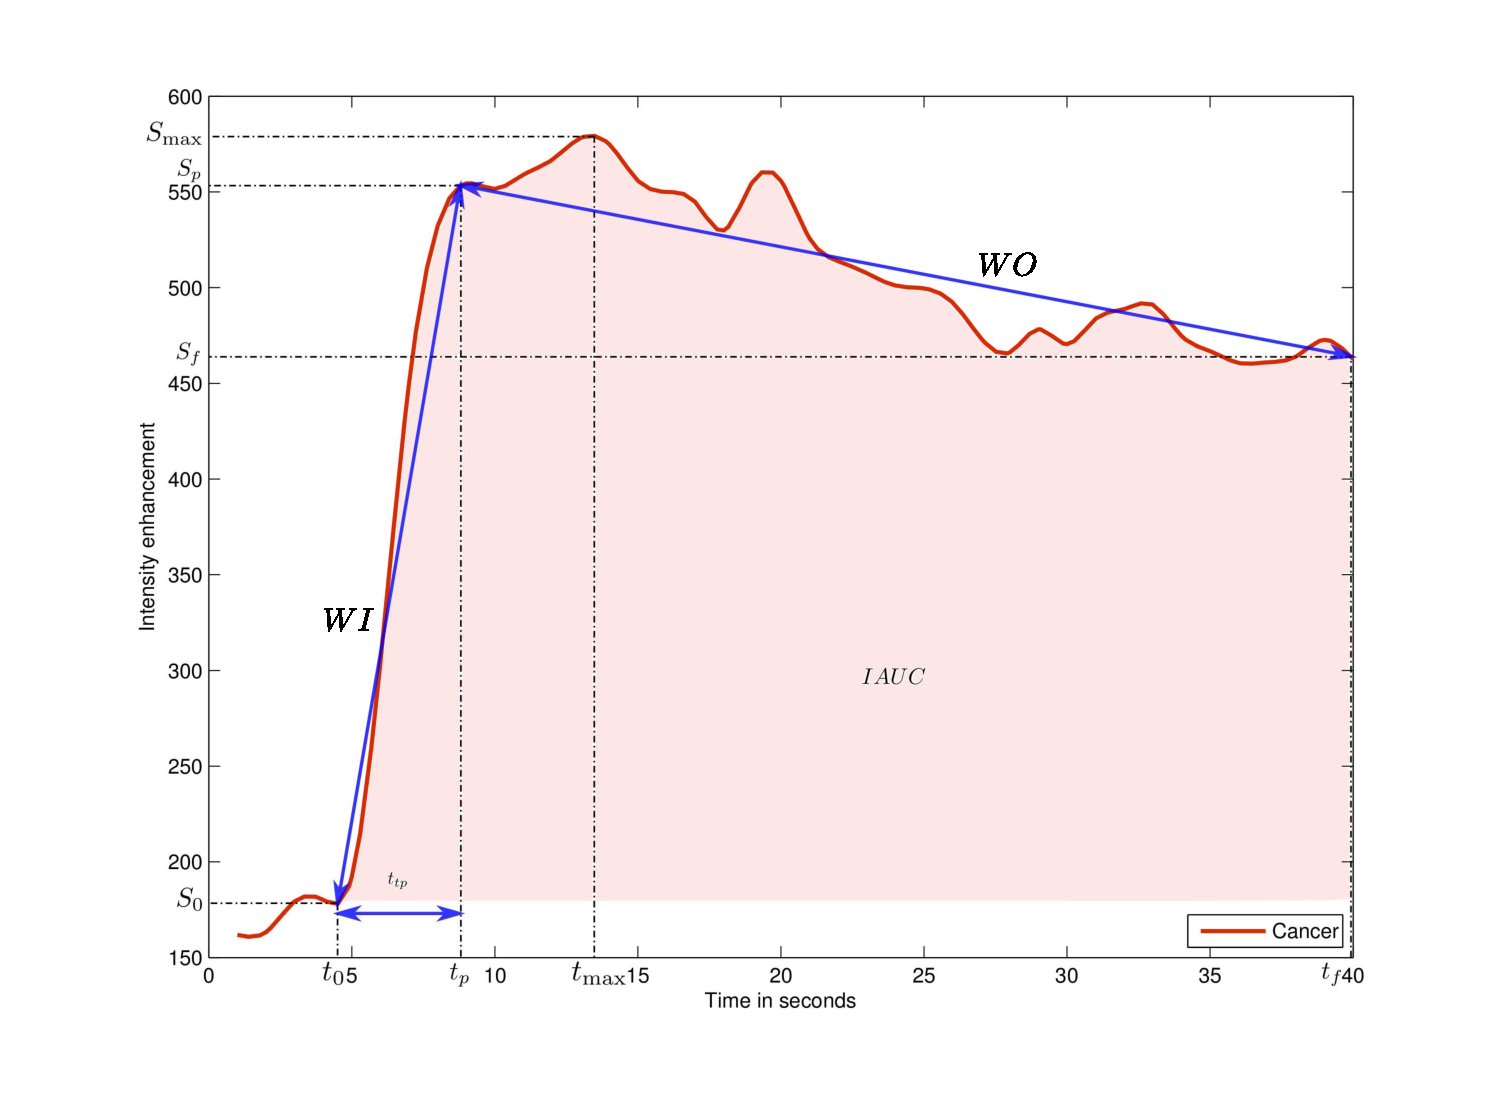
\includegraphics[width=.8\linewidth]{3_review/figures/feature-detection/dce/dce_cancer_parameters.eps}
	\caption[Semi-quantitative features used for \acs*{dce}-\acs*{mri}.]{Graphical representation of the different semi-quantitative features used for \acs*{dce}-\acs*{mri} analysis.}
	\label{fig:dceparam}
\end{figure}

\paragraph{Semi-quantitative approach}
Semi-quantitative approaches are based on mathematically modelling the \ac{dce} time series.
The parameters modelling the signal are commonly used, mainly due to the simplicity of their computation.
Parameters included in semi-quantitative analysis are summarized in Tab.~\ref{tab:semiqua} and also graphically depicted in Fig.~\ref{fig:dceparam}.
A set of time features corresponding to specific amplitude level (start, maximum and end) are extracted.
Then, derivative and integral features are also considered as discriminative and are commonly computed.


\paragraph{Quantitative approach}
As presented in Sect.~\ref{sec:chp2:imaging}, quantitative approaches correspond to mathematical-pharmacokinetic models based on physiological exchanges.
Four different models have been used in \ac{cad} for \ac{cap} systems.
The most common model reviewed was the \textit{Brix model} \cite{Artan2009,Artan2010,Sung2011,Liu2009,Ozer2009,Ozer2010}.
This model is formalized such as:
\begin{equation}
	\frac{S(t)}{S(0)} = 1 + A k_{ep} \left( \frac{\exp( -k_{ep} t ) - \exp( -k_{el} t )}{k_{el} - k_{ep}} \right) \ ,
	\label{eq:brixmod}
\end{equation}

\noindent where $S(\cdot)$ is the \ac{dce} signal, $A$ is the parameter simulating the tissue properties, $k_{el}$ is the parameter related to the first-order elimination from the plasma compartment and $k_{ep}$ is the parameter of the transvascular permeability.
These parameters ($k_{ep}$, $k_{el}$,$A$) are computed from the \ac{mri} data and used as features.

Another model is Tofts model \cite{Tofts1997} which was used in \cite{Langer2009,Giannini2013,Niaf2011,Niaf2012,Mazzetti2011}.
In this model, the \ac{dce} signal relative to the concentration is presented as:
\begin{equation}
	C_t(t) = v_p C_p(t) + K_{trans} \int_{0}^{t} C_p(\tau) \exp( -k_{ep}(t-\tau) ) \ d\tau \ ,
	\label{eq:tofts} 
\end{equation}

\noindent where $C_t(\cdot)$ is the concentration of the medium, $C_p(\cdot)$ is the \ac{aif} which have to be estimated independently, $K_{trans}$ is the parameter related to the diffuse transport of media across the capillary endothelium, $k_{ep}$ is the parameter related to the exchanges back into the vascular space and $v_e$ is the extravascular-extracellular space fraction defined such that $v_e = 1 - v_p$.
In this model, paramteres $K_{trans}$, $k_{ep}$ and $v_e$ are computed and used as features.

%Mazzetti \textit{et al.}~\cite{Mazzetti2011} and Giannini \textit{et al.}~\cite{Giannini2013} used the Weibull function empirically formalized as:
Mazzetti \textit{et al.}~\cite{Mazzetti2011} and Giannini \textit{et al.}~\cite{Giannini2013} used the Weibull function in different emprical model based on West-like function and referred to as the phenomenological universalities model \cite{Castorina2006} defined by three parameters $\beta$, $a_{0}$, and $r$ ( see Eq.~\ref{eq:pun}).

%% \begin{equation}
%% 	S(t) = A t \exp( -t^{B} ) \ ,
%% 	\label{eq:weibull}
%% \end{equation}

%% \noindent where $A$ and $B$ are the two parameters which have to be inferred.
%They also used another empirical model which is based on the West-like function and named the phenomenological universalities model \cite{Castorina2006}) formalized as:
\begin{equation}
	S(t) = \exp \left[ r t + \frac{1}{\beta} a_0 - r \left( \exp( \beta t ) - 1 \right) \right] \ ,
	\label{eq:pun}
\end{equation}
%\noindent where the parameters $\beta$, $a_0$ and $r$ are inferred.
\noindent For all these models, the parameters are inferred using an optimization curve fitting approach.


\subsubsection{\Ac{mrsi}-based features}\label{subsubsec:chp3:img-clas:CADX-fea-dec:MRSI-fea}

\paragraph{Whole spectra approach}
As in the case of \ac{dce} analysis, one common approach is to incorporate the whole \ac{mrsi} spectra in the feature vector for classification \cite{Kelm2007,Parfait2012,Tiwari2007,Tiwari2009,Tiwari2013,Tiwari2009a,Tiwari2010,Viswanath2008a,Matulewicz2013}. 
Sometimes post-processing involving dimension reduction methods is performed to reduce the complexity during the classification as it will be presented in Sect.~\ref{subsec:chp3:img-clas:CADX-fea-ext}.

\paragraph{Quantification approach}
We can reiterate that in \ac{mrsi} only few biological markers (cf., choline, creatine and citrate metabolites mainly) are known to be useful to discriminate \ac{cap} and healthy tissue.
Then, concentrations of these metabolites can be considered as a feature used for classification.
In order to perform this quantification, four different approaches have been used.
The QUEST \cite{Ratiney2005}, AMARES \cite{Vanhamme1997} and VARPRO \cite{Coleman1993} models were used in \cite{Kelm2007}.
They are all time-domain quantification methods varying by the type of pre-knowledge embedded and the optimization approaches used to solve the quantification problem.
Unlike the time-domain quantification approaches, Parfait \textit{et al.}~\cite{Parfait2012} used the LcModel approach \cite{Provencher1993}) which solves the optimization problem in the frequency domain.

Although Parfait \textit{et al.}~\cite{Parfait2012} used each metabolite concentration individually, other authors such as Kelm \textit{et al.}~\cite{Kelm2007} proposed to compute relative concentrations as the ratio of the choline plus creatine to citrate (see Eq.~\eqref{eq:ratio1}) or the ratio of citrate to choline plus creatine plus citrate (see Eq.~\eqref{eq:ratio2}).

\begin{eqnarray}
	R_1 & = & \frac{ [ \text{Cho} ] + [ \text{Cr} ]}{[ \text{Cit} ]} \ . \label{eq:ratio1} \\
	R_2 & = & \frac{[ \text{Cit} ]}{[\text{Cho}]+[\text{Cr}]+[\text{Cit}]} \ , \label{eq:ratio2}
\end{eqnarray}
\noindent where $\text{Cit}$, $\text{Cho}$ and $\text{Cr}$ are the concentration of citrate, choline and creatine respectively.

\paragraph{Wavelet decomposition approach} 
Tiwari \textit{et al.}~\cite{Tiwari2012} performed a wavelet packet decomposition \cite{Coifman1992} of the spectra with the Haar wavelet basis function and used its coefficients as features.

\subsection{\acs*{cadx}: Feature selection and feature extraction} \label{subsec:chp3:img-clas:CADX-fea-ext}
As presented in the previous section, it is a common practise to extract a wide variety of features.
While dealing with \ac{mpmri}, the feature space created is a high-dimensional space which might mislead or corrupt the classifier during the training phase.
Therefore, it is of interest to reduce the number of dimensions before proceeding to the classification task.
The strategies used can be grouped as: (i) feature selection and (ii) feature extraction.
In this section only the methods used in \ac{cad} system are presented and summarized in \acs{tab}~\ref{tab:featext}.

\begin{table}
  \caption{Overview of the feature selection and extraction methods used in \acs*{cad} systems.}
  \scriptsize
  \centering
  \begin{tabular}{l r}
    \toprule
    \textbf{Dimension reduction methods} & \textbf{References} \\
    \midrule
    \textbf{Feature selection:} & \\ \\ [-1.5ex]
    \quad Statistical test & \cite{Niaf2011,Niaf2012,Vos2012} \\
    \quad \ac{mi}-based methods & \cite{Niaf2011,Niaf2012,Vos2008,lehaire2014computer,khalvati2015automated,chung2015prostate} \\
    \quad Correlation-based methods & \cite{rampun2016computer,rampun2015computer} \\ \\ [-1.5ex]
    \textbf{Feature extraction:} & \\ \\ [-1.5ex]
    \quad Linear mapping & \\
    \quad \quad \acs*{pca} & \cite{Tiwari2008,Tiwari2009} \\
    \quad Non-linear mapping & \\
    \quad \quad Laplacian eigenmaps & \cite{Tiwari2007,Tiwari2009a,Tiwari2009,Tiwari2010,Viswanath2008,Viswanath2011} \\
    \quad \quad \acs*{lle} and \acs*{lle}-based & \cite{Tiwari2008,Tiwari2009,Viswanath2008a,Viswanath2008} \\
    \quad Dictionary-based learning & \\
    \quad \quad Sparse coding & \cite{lehaire2014computer} \\
    \quad \quad \acs*{bow} & \cite{rampun2016computerb,rampun2015classifying} \\
    \bottomrule
  \end{tabular}
\label{tab:featext}
\end{table} 

\subsubsection{Feature selection}\label{subsubsec:chp3:img-clas:CADX:fea-ext:sel}
The feature selection strategy is based on selecting the most discriminative feature dimensions of the high-dimensional space.
Thus, the low-dimensional space is then composed of a subset of the original features detected.
In this section, methods employed in \ac{cad} for \ac{cap} detection are presented.
A more extensive review specific to feature selection is available in~\cite{Saeys2007}.

\citeauthor{Niaf2012} make use of the p-value by using the independent two-sample t-test with equal mean for each feature dimension~\cite{Niaf2011,Niaf2012}.
In this statistical test, there are 2 classes: \ac{cap} and healthy tissue.
Hence, for each particular feature, the distribution of each class is characterized by their means $\bar{X}_1$ and $\bar{X}_2$ and standard deviation $s_{X_1}$ and $s_{X_2}$.
Therefore, the null hypothesis test is based on the fact that these both distribution means are equal.
The t-statistic used to verify the null hypothesis is formalized such that:

\begin{eqnarray}
t & = & \frac{\bar {X}_1 - \bar{X}_2}{s_{X_1X_2} \cdot \sqrt{\frac{1}{n_1}+\frac{1}{n_2}}} \ , \label{eq:tstat} \\
s_{X_1X_2} & = & \sqrt{\frac{(n_1-1)s_{X_1}^2+(n_2-1)s_{X_2}^2}{n_1+n_2-2}} \ , \nonumber
\end{eqnarray}

\noindent where $n_1$ and $n_2$ are the number of samples in each class.
From \acs{eq}\,\eqref{eq:tstat}, more the means of the class distribution diverge, the larger the $t$-statistic $t$ will be, implying that this particular feature is more relevant and able to make the distinction between the two classes. 

The $p$-value statistic is deduced from the $t$-test and corresponds to the probability of obtaining such an extreme test assuming that the null hypothesis is true~\cite{Goodman1999}.
%Hence, smaller the $p$-value, the more likely we are to reject the null hypothesis and more relevant the feature is likely to be.
Hence, smaller the $p$-value, the more likely the null hypothesis to be rejected the null hypothesis and more relevant the feature is likely to be.
Finally, the features are ranked and the most significant features are selected.
However, this technique suffers from a main drawback since it assumes that each feature is independent, which is unlikely to happen and introduces a high degree of redundancy in the features selected.

\citeauthor{Vos2012} in~\cite{Vos2012} employed a similar feature ranking approach but make use of the Fisher discriminant ratio to compute the relevance of each feature dimension.
Taking the aforementioned formulation, the Fisher discriminant ratio is formalized as the ratio of the interclass variance to the intraclass variance as:

\begin{equation}
F_r = \frac{\bar{X}_1 - \bar{X}_2}{s^{2}_{X_1}+s^{2}_{X_2}} \ .
\label{eq:fisherratio}
\end{equation}

Therefore, a relevant feature dimension is selected when the interclass variance is maximum and the intraclass variance in minimum.
Once the features are ordered, the authors select the feature dimensions with the largest Fisher discriminant ratio.

\Ac{mi} is a possible metric to use for selecting a subset of feature dimensions.
This method has previously been presented in \acs{sec}\,\ref{subsec:chp3:img-reg:reg} and expressed in \acs{eq}\,\eqref{eq:midef}.
%%%% As previously presented in Sect.~\ref{subsec:chp3:img-reg:reg} (see Eq.~\eqref{eq:midef}), the computation of the entropies involves the estimation of some \acp{pdf} and the data being usually continous variables, it is then necessary to estimate the \acp{pdf} using a method such as Parzen windows.
%%%% Definition of the \ac{mi} was presented in Sect.~\ref{subsec:chp3img-reg:reg} and formalized in Eq. \eqref{eq:midef} and as previously mentioned, the computation of the entropies involves the estimation of some \acp{pdf} and the data being usually continuous variables, it is then necessary to estimate the \acp{pdf} using a method such as Parzen windows.
\citeauthor{Peng2005} introduced two main criteria to select the feature dimensions based on \ac{mi}: (i) maximal relevance and (ii) minimum redundancy.
Maximal relevance criterion is based on the paradigm that the classes and the feature dimension which has to be selected have to share a maximal \ac{mi} and is formalized as:
\begin{equation}
  \argmax Rel(\mathbf{x},c) = \frac{1}{|\mathbf{x}|} \sum_{x_i \in \mathbf{x}} MI(x_i,c)  \ , 
  \label{eq:mRel}
\end{equation}
\noindent where $\mathbf{x} = \{x_i; i=1,\cdots,d\}$ is a feature vector of $d$ dimensions and $c$ is the class considered.
As in the previous method, using maximal relevance criterion alone imply an independence between each feature dimension.
The minimal redundancy criterion enforce the selection of a new feature dimension which shares as little as possible \ac{mi} with the previously selected feature dimensions such that:
\begin{equation}
  \argmin Red(\mathbf{x}) = \frac{1}{|\mathbf{x}|^2} \sum_{x_i,x_j \in \mathbf{x}} MI(x_i,x_j)  \ . 
  \label{eq:mRed}
\end{equation}
Combination of these two criteria is known as the \ac{mrmr} algorithm~\cite{Peng2005}.
Two combinations are usually used: (i) the difference or (ii) the quotient.
This method has been used at several occasions for the selecting a subset of features prior to classification~\cite{Niaf2011,Niaf2012,lehaire2014computer,Viswanath2012,khalvati2015automated,chung2015prostate}.

{\color{red} add a couple of sentence about correlation-based feature selection used by Rampun}.

\subsubsection{Feature extraction}\label{subsubsec:chp3:img-clas:CADX:fea-ext:ext}
The feature extraction strategy is related to dimension reduction methods but not selecting discriminative features.
Instead, these methods aim at mapping the data from the high-dimensional space into a low-dimensional space to maximize the separability between the classes.
As in the previous sections, only methods employed in \ac{cad} system are reviewed in this section.
We refer the reader to~\cite{Fodor2002} for a full review of feature extraction techniques.

\ac{pca} is the most commonly used linear mapping method in \ac{cad} systems.
\ac{pca} is based on finding the orthogonal linear transform mapping the original data into a low-dimensional space.
The space is defined such that the linear combinations of the original data with the $k^{th}$ greatest variances lie on the $k^{th}$ principal components~\cite{Jolliffe2002}.
The principal components are computed by using the eigenvectors-eigenvalues decomposition of the covariance matrix.
Let $\mathbf{x}$ denote the data matrix.
Then, the covariance matrix and eigenvectors-eigenvalues decomposition are defined as in \acs{eq}\,\eqref{eq:covmat}, and \acs{eq}\,\eqref{eq:eigpca}, respectively. 
The eigenvectors-eigenvalues decomposition can be formalized as:
\begin{equation}
  \Sigma = \mathbf{x}^{\text{T}} \mathbf{x} \ .
  \label{eq:covmat}
\end{equation}

\begin{equation}
  \mathbf{v}^{-1} \Sigma \mathbf{v} = \Lambda \ ,
  \label{eq:eigpca}
\end{equation}
\noindent where $\mathbf{v}$ are the eigenvectors matrix and $\Lambda$ is a diagonal matrix containing the eigenvalues. 

It is then possible to find the new low-dimensional space by sorting the eigenvectors using the eigenvalues and finally select the eigenvectors corresponding to the largest eigenvalues.
The total variation that is the sum of the principal eigenvalues of the covariance matrix~\cite{Fodor2002}, usually corresponds to the \SIrange{95}{98}{\percent} of the cumulative sum of the eigenvalues.
\citeauthor{Tiwari2012} used \ac{pca} in order to reduce the complexity of feature space~\cite{Tiwari2008,Tiwari2009,Tiwari2012}.

Non-linear mapping has been also used for dimension reduction and is mainly based on Laplacian eigenmaps and \acf{lle} methods.
Laplacian eigenmaps also referred as spectral clustering in computer vision, aim to find a low-dimensional space in which the proximity of the data should be preserved from the high-dimensional space~\cite{Shi2000,Belkin2001}.
Therefore, two adjacent data points in the high-dimensional space should also be close in the low-dimensional space.
Similarly, two distant data points in the high-dimensional space should also be distant in the low-dimensional space.
To compute this projection, an adjacency matrix is defined as:
\begin{equation}
	W(i,j) = \exp \| \mathbf{x}_i - \mathbf{x}_j \|_2 \ ,
	\label{eq:gew}
\end{equation}

\noindent where $\mathbf{x}_i$ and $\mathbf{x}_j$ are the two samples considered.
Then, the low-dimensional space is found by solving the generalized eigenvectors-eigenvalues problem:

\begin{equation}
	(D-W)\mathbf{y} = \lambda D \mathbf{y} \ ,
	\label{eq:geeig}
\end{equation}

\noindent where $D$ is a diagonal matrix such that $D(i,i) = \sum_j W(j,i)$.
Finally the low-dimensional space is defined by the $k$ eigenvectors of the $k$ smallest eigenvalues~\cite{Belkin2001}.
\citeauthor{Tiwari2009a} and \citeauthor{Viswanath2008} used this spectral clustering to project their feature vector into a low-dimensional space~\cite{Tiwari2007,Tiwari2009,Tiwari2009a,Viswanath2008}.
The feature space in these studies is usually composed of features extracted from a single or multiple modalities and then concatenated before applying the Laplacian eigenmaps dimension reduction technique.

\citeauthor{Tiwari2013} used a slightly different approach by combining the Laplacian eigenmaps techniques with a prior multi-kernel learning strategy~\cite{Tiwari2009,Tiwari2013}.
First, multiple features are extracted from multiple modalities.
The features of a single modality are then mapped to a higher-dimensional space via the Kernel trick~\cite{Aizerman1964}, namely a Gaussian kernel.
Then, each kernel is linearly combined to obtain a combined kernel $K$ and the adjacency matrix $W$ is computed.
Finally, the same scheme as in the Laplacian eigenmaps is applied.
However, in order to use the combined kernel, \acs{eq}\,\eqref{eq:geeig} is rewritten as:

\begin{equation}
  K (D-W) K^{\text{T}} \mathbf{y} = \lambda K D K^{\text{T}} \mathbf{y} \ ,
  \label{eq:sesmik}
\end{equation}
\noindent which is solved as a generalized eigenvectors-eigenvalues problem as previously.
\citeauthor{Viswanath2011} used Laplacian eigenmaps inside a bagging framework in which multiple embeddings are generated by successively selecting feature dimensions~\cite{Viswanath2011}.

\Ac{lle} is another common non-linear dimension reduction technique widely used, first proposed in~\cite{Roweis2000}.
\ac{lle} is based on the fact that a data point in the feature space is characterized by its neighbourhood.
Thus, each data point in the high-dimensional space is transform to represent a linear combination of its $k$-nearest neighbours.
This can be expressed as:
\begin{equation}
	\hat{\mathbf{x}}_i = \sum_j W(i,j) \mathbf{x}_j \ ,
	\label{eq:lincomlle}
\end{equation}

\noindent where $\hat{\mathbf{x}}_i$ are the data point estimated using its neighbouring data points $\mathbf{x}_j$, and $W$ is the weight matrix.
The weight matrix $W$ is estimated using a least square optimization as in \acs{eq}\,\eqref{eq:lslle}.
%Hence, this problem which has to be solved at this stage is to estimate the weight matrix $W$. This problem can be tackled using a least square optimization scheme by optimizing the following objective function:
\begin{eqnarray}
	\hat{W} & = & \argmin_{W} \sum_i | \mathbf{x}_i - \sum_j W(i,j)\mathbf{x}_j |^{2} \ , \label{eq:lslle} \\
	&& \text{subject to } \sum_j W(i,j) = 1 \ , \nonumber
\end{eqnarray}

Then, the essence of \ac{lle} is to project the data into a low-dimensional space, while retaining the data saptial organization.
Therefore, the projection into the low-dimensional space is tackled as an optimization problem as:

\begin{equation}
	\hat{\mathbf{y}} = \argmin_{\mathbf{y}} \sum_i | \mathbf{y}_i - \sum_j W(i,j)\mathbf{y}_j |^{2} \ .
	\label{eq:lowprojlle}
\end{equation}

This optimization is solved as an eigenvectors-eigenvalues problem by finding the $k^{\text{th}}$ eigenvectors corresponding to the $k^{\text{th}}$ smallest eigenvalues of the sparse matrix $(I-W)^{\text{T}}(I-W)$.

\citeauthor{Tiwari2008} used a modified version of the \ac{lle} algorithm in which they applied \ac{lle} in a bagging approach with multiple neighbourhood sizes~\cite{Tiwari2008}.
The different embeddings obtained are then fused using the \ac{ml} estimation.

Another way of reducing the complexity of high-dimensional feature space is to use the family of so-called dictionary-based methods.
\Ac{scf} representation has become very popular in other computer vision application and has been used by \citeauthor{lehaire2014computer} in~\cite{lehaire2014computer}.
The main goal of sparse modeling is to efficiently represent the images as a linear combination of a few typical patterns, called atoms, selected from a dictionary.
Sparse coding consists of three main steps: (i) dictionary learning and low-level features projection~\cite{rubinstein2008efficient}.

\emph{Sparse approximation -} Given a dictionary $\mathbf{D} \in \mathbb{R}^{n \times K}$ composed of $K$ atoms and an original signal $\mathbf{y} \in \mathbb{R}^{n}$ --- i.e., one feature vector ---, the sparse approximation corresponds to find the sparest vector $\mathbf{x} \in \mathbb{R}^{K}$ such that:

\begin{equation}
  \argmin_{\mathbf{x}}\|\mathbf{y - Dx} \|_{2} \qquad  \text{s.t.} \  \|\mathbf{x}\|_{0} \leq \lambda \, \label{eq:sprapp} \ ,
\end{equation}
\noindent where $\lambda$ is a specified sparsity level.

Solving the above optimization problem is an NP-hard problem~\cite{elad2010sparse}.
However, approximate solutions are obtained using greedy algorithms such as \ac{mp}~\cite{mallat1993matching} or \ac{omp}~\cite{pati1993orthogonal,davis1997adaptive}.

\emph{Dictionary learning -} As stated previously, the sparse approximation is computed given a specific dictionary $\mathbf{D}$, which involves a learning stage from a set of training data.
This dictionary is learned using $K$-\acs*{svd} which is a generalized version of $K$-means clustering and uses \ac{svd}. 
The dictionary is built, in an iterative manner by solving the optimization problem of \acs{eq}\,\eqref{eq:dct}, by alternatively computing the sparse approximation of $\mathbf{X}$ and the dictionary $\mathbf{D}$.
\begin{equation}
  \argmin_{\mathbf{D,X}} \|\mathbf{Y} - \mathbf{D}\mathbf{X}\|_{2} \qquad  \text{s.t.} \  \|\mathbf{x}_{i}\|_{1} \leq \lambda \,\label{eq:dct} \ ,
\end{equation}
\noindent where $\mathbf{Y}$ is a training set of low-level descriptors, $\mathbf{X}$ is the associated sparse coded matrix --- i.e., set of high-level descriptors --- with a sparsity level $\lambda$, and $\mathbf{D}$ is the dictionary with $K$ atoms.
Given $\mathbf{D}$, $\mathbf{X}$ is computed using the batch-\ac{omp} algorithm, while given $\mathbf{X}$, $\mathbf{D}$ is sequentially updated, one atom at a time using \ac{svd}. 

\emph{Low-level features projection -} Once the dictionary is learned, each set of low-level features $\mathbf{F}_{I}$ previously extracted is encoded using the dictionary $\mathbf{D}$, solving the optimization problem presented in \acs{eq}\,\eqref{eq:sprapp} such that $\mathbf{F}_{I} \simeq \mathbf{DX}_{I}$.

\ac{bow} approach offer an alternative methods~\cite{Sivic2003} which has been used by \citeauthor{rampun2016computerb} in~\cite{rampun2015classifying}.
This model represents the features by creating a codebook or visual dictionary, from the set of low-level features.
The set of low-level features are clustered using \textit{k}-means to create the dictionary with \textit{k} clusters known as visual words.
Once the codebook created from the training set, the low-level descriptors are replaced by their closest word within the codebook.
The final descriptor is a histogram of size \textit{k} which represents the codebook occurrences for a given mapping.

% THIS IS FROM MY THESIS, YOU CAN USE THIS, If you like

%% \acf{scf}, or sparse signal representation, has become very popular over the past few decades and has led to state-of-the-art results in various applications such as face recognition~\cite{wright2009robust}, image denoising, image inpainting~\cite{elad2006image}, and image classification~\cite{sidibe2015discrimination}. 
%% The main goal of sparse modeling is to efficiently represent the samples/images as a linear combination of a few typical patterns, called atoms, selected from the dictionary.
%% Sparse coding consists of three main steps: (i) dictionary learning, (ii) low-level feature projection, and (iii) feature pooling~\cite{rubinstein2008efficient}. 
%% Considering our dictionary $D \in R^{n \times K}$ with $K$ atoms, where each column of $D$ represents one atom, the sparse coding problem of a signal $y \in R^{n}$ is defined as finding the sparsest vector $x$ so that $y \approx Dx$. 
%% This is an optimization problem that can be formulated as:
%% \begin{equation}
%% \min_{x} \|y-Dx\|_{2} \qquad \text{s.t.}\ \|x\|_{0} \leq \lambda \,,
%% \end{equation}  
%% \noindent where $\lambda$ is the sparsity level and $l^{0}$-norm accounts for the minimum number of non-zero elements in the sparse vector $x$. 
%% This optimization problem is NP hard~\cite{Elad2010}, subsequently approximation solutions are proposed either by using greedy algorithms such as \ac{mp}~\cite{mallat1993matching} and \ac{omp}~\cite{davis1994adaptive}, or by replacing the $l^{0}$-norm with $l^{1}$-norm such as in the \ac{bp} algorithm~\cite{chen1998atomic}.
%% %\noindent where $\lambda$ is the sparsity level and $l^{0}$-norm accounts for the minimum number of non-zero elements in sparse vector $x$. 
%% %This optimization problem is NP hard~\cite{Elad2010}.
%% %Subsequently approximation solutions are proposed either by using greedy algorithms such as \ac{mp}~\cite{mallat1993matching} and \ac{omp}~\cite{davis1994adaptive} or by replacing the $l^{0}$-norm with $l^{1}$-norm such as \ac{bp}~\cite{chen1998atomic}.
%% The dictionary is learned using K-SVD, a generalized version of \textit{k}-means clustering that uses \ac{svd}~\cite{aharon2006img}. 
%% The dictionary is built such that:
%% \begin{equation}
%%   \min_{Dx} \|y - Dx\|_{2} \qquad  \text{s.t.} \ \forall i \ \|x_{i}\|_{1} \leq \lambda \,,
%% \end{equation}

%% \noindent where $y$ is a low-level descriptor, $x$ is the sparse coded descriptor (i.e., high-level descriptor) with a sparsity level $\lambda$, and $D$ is the dictionary with $K$ atoms.
%% The K-SVD algorithm solves the optimization problem iteratively by alternating between $x$ and $D$. 
%% With $D$, the sparse code matrix $x$ is computed by any of the pursuit algorithms, and with $x$, $D$ is updated one atom at a time using \ac{svd}. 

%% Once the dictionary is learned, each $y_{i} \in R^{n}$ signal can be projected using $D$ to form a set of sparse codes $x_{i} \in R^{K}$. 
%% In the case of image samples, the sparse representation can be generated for patches in the image.
%% In this case, the final mapping is based on a combination of sparse codes, for instance by taking the maximum code from all the patches: 
%% \begin{equation}
%% f_{i} = \max_{j}(\vert X_{l}(i,j)\vert) \qquad  \forall  i = 1, 2, .., K \,,
%% \end{equation} 
%% \noindent where $X_{l} \in R^{K \times P}$ is the sparse code matrix~\cite{sidibe2015discrimination}. 
%% \end{description}

\subsection{\acs*{cadx}: Classification} \label{subsec:chp3:img-clas:CADX-clas}

%\subsubsection{Classifier} \label{subsubsec:chp3:img-clas:CADX-clas:clas}

Once the feature vector has been extracted and eventually the complexity reduced, it is possible to make a decision and classify this feature vector to belong to \ac{cap} or healthy tissue.
A full review of classification methods used in pattern recognition is available in~\cite{Bishop2006}.

\paragraph{Rule-based method}
\citeauthor{Lv2009} make use of a decision stump classifier to distinguish \ac{cap} and healthy classes~\cite{Lv2009}. 
\citeauthor{Puech2009} detect \ac{cap} by implementing a given set of rules and scores based on a medical support approach~\cite{Puech2009}.
During the testing, the feature vector goes through these different rules, and a final score is computed resulting to a final decision.

\paragraph{Clustering methods}
\acf{knn} is one of the simplest supervised machine learning classification methods.
In this method, a new unlabelled vector is assigned to the most represented class from its $k$ nearest-neighbours in the feature space.
The parameter $k$ is usually an odd number in order to avoid any tie case.
\ac{knn} has been one of the methods used in~\cite{Niaf2011,Niaf2012,rampun2016computerb} mainly to make a comparison with different machine learning techniques.
\citeauthor{Litjens2012} used this method to roughly detect potential \ac{cap} voxels before performing a region-based classification~\cite{Litjens2012}.

The $k$-means algorithm is an unsupervised clustering method in which the data is partitioned into $k$ clusters in an iterative manner.
First, $k$ random centroids are defined in the feature space and each data point is assigned to the nearest centroid.
Then, the centroid position for each cluster is updated by computing the mean of all the samples belonging to this particular cluster.
Both assignment and updating are repeated until the centroids are stable.
The number of clusters $k$ is usually defined as the number of classes.
This algorithm can also be used for ``on-line'' learning.
In case that new data has to be incorporated, the initial centroid positions correspond to the results of a previous $k$-means training and is followed by the assignment-updating stage previously explained.
\citeauthor{Tiwari2009} used $k$-means in an iterative procedure~\cite{Tiwari2007,Tiwari2009}.
Three clusters were defined corresponding to \ac{cap}, healthy, and non-prostate.
$k$-means is repeatedly applied and at each iteration, the voxels corresponding to the largest cluster are excluded under the assumption that it is assigned to ``non-prostate'' cluster.
The algorithm stopped when the number of voxels in all remaining clusters were smaller than a given threshold.
\citeauthor{Tiwari2008} and \citeauthor{Viswanath2008a} used $k$-means in a repetitive manner in order to be less sensitive to the centroids initialization~\cite{Viswanath2008,Viswanath2008a,Tiwari2008}.
Thus, $k$ clusters are generated $T$ times and the final assignment is performed by majority voting using a co-association matrix as proposed in~\cite{Fred2005}.

\paragraph{Linear model classifiers}
\Acf{lda} is used as a classification method in which the optimal linear separation between 2 classes is found by maximizing the inter-class variance and minimizing the intra-class variance~\cite{Friedman1989}.
The linear discriminant function is defined as:
\begin{equation}
	\delta_{k}(\mathbf{x}_i) = \mathbf{x}_i^{\text{T}} \Sigma^{-1} \mu_k - \frac{1}{2} \mu_{k}^{\text{T}} \Sigma^{-1} \mu_k + \log (\pi_k) \ ,
	\label{eq:ldafun}
\end{equation}

\noindent where $\mathbf{x}_i = \{x_1, x_2, \dots , x_n\}$ is an unlabelled feature vector of $n$ features, $\Sigma$ is the covariance matrix of the training data, $\mu_k$ is the mean vector of the class $k$, and $\pi_k$ is the prior probability of class $k$.
To perform the classification, a sample $\mathbf{x}_i$ is assigned to the class which maximizes the discriminant function as in \acs{eq}\,\eqref{eq:ldaclass}.
\begin{equation}
	C(\mathbf{x}_i) = \argmax_k \delta_k(\mathbf{x}_i) \ .
	\label{eq:ldaclass}
\end{equation}
\Ac{lda} has been used in~\cite{Antic2013,Chan2003,Niaf2011,Niaf2012,Vos2012}.

%covariance matrix $\Sigma_k$ specific at each class is computed.
%used \ac{lda} to classify their feature vectors defining two classes \ac{cap} \textit{versus} healthy

Logistic regression is also used to perform binary classification and provides the probability of an observation to belong to a class.
The posterior probability of one of the classes, $c_1$ is written as:
\begin{equation}
	p(c_1|\mathbf{x}_i) = \frac{1}{1+\exp(-\mathbf{w}^{\text{T}}\mathbf{x}_i)} \ ,
	\label{eq:postprlr}
\end{equation}

\noindent with $p(c_2|\mathbf{x}_i) = 1 - p(c_1|\mathbf{x}_i)$ and where $\mathbf{w}$ is the vector of the regression parameters allowing to obtain a linear combination of the input feature vector $\mathbf{x}_i$.
Thus, an unlabelled observation $\mathbf{x}_i$ is assigned to the class which maximizes the posterior probability as shown in \acs{eq}\,\eqref{eq:posprobreg}.

\begin{equation}
	C(\mathbf{x}_i) = \argmax_k p(C=k|\mathbf{x}_i) \ .
	\label{eq:posprobreg}
\end{equation}

From \acs{eq}\,\eqref{eq:postprlr}, one can see that the key to classification using logistic regression model is to infer the set of parameters $\mathbf{w}$ through a learning stage using a training set.
This vector of parameters $\mathbf{w}$ is inferred by estimating the maximum likelihood.
This step is performed through an optimization scheme, using a quasi-Newton method~\cite{Byrd1995}, which seeks in an iterative manner for the local minimum in the derivative of \acs{eq}\,\eqref{eq:postprlr}.
This method has been used to create a linear probabilistic model in~\cite{Kelm2007,Puech2009,lehaire2014computer,rampun2015computer}.

\paragraph{Non-linear model classifier}
\citeauthor{Viswanath2012} used \acf{qda} instead of \ac{lda}~\cite{Viswanath2012}.
Unlike in \ac{lda} in which one assumes that the class covariance matrix $\Sigma$ is identical for all classes, a covariance matrix $\Sigma_k$ specific to each class is computed.
Thus, \acs{eq}\,\eqref{eq:ldafun} becomes:
\begin{equation}
	\delta_{k}(\mathbf{x}_i) = \mathbf{x}_i^{\text{T}} \Sigma_{k}^{-1} \mu_k - \frac{1}{2} \mu_{k}^{\text{T}} \Sigma_{k}^{-1} \mu_k + \log (\pi_k) \ ,
	\label{eq:qdafun}
\end{equation}

\noindent where $\mathbf{x}_i$ has additional terms corresponding to the pairwise products of individual features such as $\{x_1, x_2, \dots , x_n, x_1^2, x_1x_2, \dots x_n^2\}$.
The classification scheme in the case of the \ac{qda} is identical to \acs{eq}\,\eqref{eq:ldaclass}.

\paragraph{Probabilistic classifiers}
The most commonly used classifier is the naive Bayes classifier which is a probabilistic classifier assuming independence between each feature dimension~\cite{Rish2001}.
This classifier is based on Bayes' theorem:

\begin{equation}
	p(C=k|\mathbf{x}) = \frac{p(C)p(\mathbf{x}|C)}{p(\mathbf{x})} \ ,
	\label{eq:bayth}
\end{equation}

\noindent where $p(C=k|\mathbf{x})$ is the posterior probability, $p(C)$ is the prior probability, $p(\mathbf{x}|C)$ is the likelihood, and $p(\mathbf{x})$ is the evidence. 
However, the evidence term is usually discarded since it is not class dependent and plays the role of a normalization term.
Hence, in a classification scheme, an unlabelled observation is classified to the class which maximizes the posterior probability as:

\begin{eqnarray}
	C(\mathbf{x}_i) & = & \argmax_k p(C=k|\mathbf{x}_i) \ , \label{eq:maxbay} \\
	p(C=k|\mathbf{x}_i) & = & p(C=k) \prod_{j=1}^{n} p(x_{ij},|C=k) \ , \label{eq:postbay}
\end{eqnarray}

\noindent where $d$ is the number of dimensions of the feature vector $\mathbf{x}_i = \{x_{i1},\cdots,x_{id}\}$.
Usually, a model includes both the prior and likelihood probabilities and it is common to use an equal prior probability for each class or eventually a value based on the relative frequency derived from the training set.
Regarding the likelihood probability, it is common to choose a Gaussian distribution to characterize each class.
Thus, each class is characterized by two parameters: (i) the mean and (ii) the standard deviation.
These parameters are inferred from the training set by using the \ac{mle} approach.
The naive Bayes classifier has been used in~\cite{Giannini2013,Mazzetti2011,Niaf2011,Niaf2012,Niaf2012,cameron2014multiparametric,cameron2016maps,rampun2015classifying,rampun2016computerb,rampun2015computer,rampun2016computer}.

\paragraph{Ensemble learning classifiers}
AdaBoost is an adaptive method based on an ensemble learning method and initially proposed in~\cite{Freund1997}. 
AdaBoost linearly combines several weak learners resulting into a final strong classifier.
A weak learner is defined as a classification method performing slightly better than a random classifier.
Popular choices regarding the weak learner classifiers are: decision stump or decision tree learners such as \ac{id3}~\cite{Quinlan1986}, C4.5~\cite{Quinlan1993}, and \ac{cart}~\cite{Breiman1984}.

AdaBoost is considered as an adaptive method in the way that the weak learners are selected.
The selection is performed in an iterative manner.
At each iteration $t$, the weak learner selected $h_t$ corresponds to the one minimizing the classification error on a distribution of weights $D_t$, that is associated with the training samples.
Each weak learner is assigned a weight $\alpha_t$ as:

\begin{equation}
	\alpha_t = \frac{1}{2} \ln \frac{1 - \epsilon_t}{\epsilon_t} \ ,
	\label{eq:wclssada}
\end{equation}

\noindent where $\epsilon_t$ corresponds to the classification error rate of the weak learner on the distribution of weight $D_t$.

Before performing a new iteration, the distribution of weights $D_t$ is updated such that the weights associated with the misclassified samples by $h_t$ increase and the weights of well classified samples decrease as shown in \acs{eq}\,\eqref{eq:rewada}.

\begin{equation}
	D_{t+1}(i) = \frac{ D_t(i) \exp \left( -\alpha_t y_i h_{t}(\mathbf{x}_{i} ) \right) }{ Z_t  } \ ,
	\label{eq:rewada} 
\end{equation}

\noindent where $\mathbf{x}_i$ is the $i^{\text{th}}$ sample corresponding to class $y_i$ and $Z_t$ is a normalization factor forcing $D_{t+1}$ to be a probability distribution. 
This procedure allows to select a weak learner at the next iteration $t+1$ which will classify in priority the previous misclassified samples. 
Thus, after $T$ iterations, the final strong classifier corresponds to the linear combination of the weak learners selected and the classification is performed such that:

\begin{equation}
	C(\mathbf{x}_i) = \sign \left( \sum_{t=1}^{T} \alpha_t h_t(\mathbf{x}_i) \right) \ .
	\label{eq:strclaada}
\end{equation}

\citeauthor{Lopes2011} make use of the AdaBoost classifier to perform their classification~\cite{Lopes2011} while \citeauthor{Litjens2014} used the GentleBoost variant~\cite{Friedman1998} which provides a modification of the function affecting the weight at each weak classifier~\cite{Litjens2014}.

\Ac{rf} is a classification method which is based on creating an ensemble of decision trees and was introduced in~\cite{Breiman2001}.
In the learning stage, multiple decision tree learners~\cite{Breiman1984} are trained.
However, each decision tree is trained using a different dataset.
Each of these datasets corresponds to a bootstrap sample generated by randomly choosing $n$ samples with replacement from the initially $N$ samples available~\cite{Efron1979}.
Then, randomization is also part of the decision tree growth.
At each node of the decision tree, from the bootstrap sample of $D$ dimensions, a number of $d \ll D$ dimensions will be randomly selected.
Finally, the $d^{\text{th}}$ dimension in which the classification error is minimum is used.
This best ``split'' classifier is often evaluated using \ac{mi} or Gini index.
Finally, each tree is grown as much as possible without using any pruning procedure.
In the prediction stage, the unlabelled sample is introduced in each tree and each of them assign a class.
Finally, it is common to use a majority voting approach to choose the final class label.
The \ac{rf} classifier has been used in~\cite{Kelm2007,Litjens2014,Tiwari2012,Tiwari2013,Viswanath2009,trigui2017automatic,trigui2016classification,samarasinghe2016semi,rampun2015classifying,rampun2016computerb,rampun2015computer,rampun2016computer}.

\begin{figure}
\centering
	\begin{tikzpicture}
    [level distance=1.75cm,sibling distance=1.5cm,scale=.95,every node/.style={scale=0.95}, 
   edge from parent path={(\tikzparentnode) -- (\tikzchildnode)}]
	\Tree [.\node (foo) {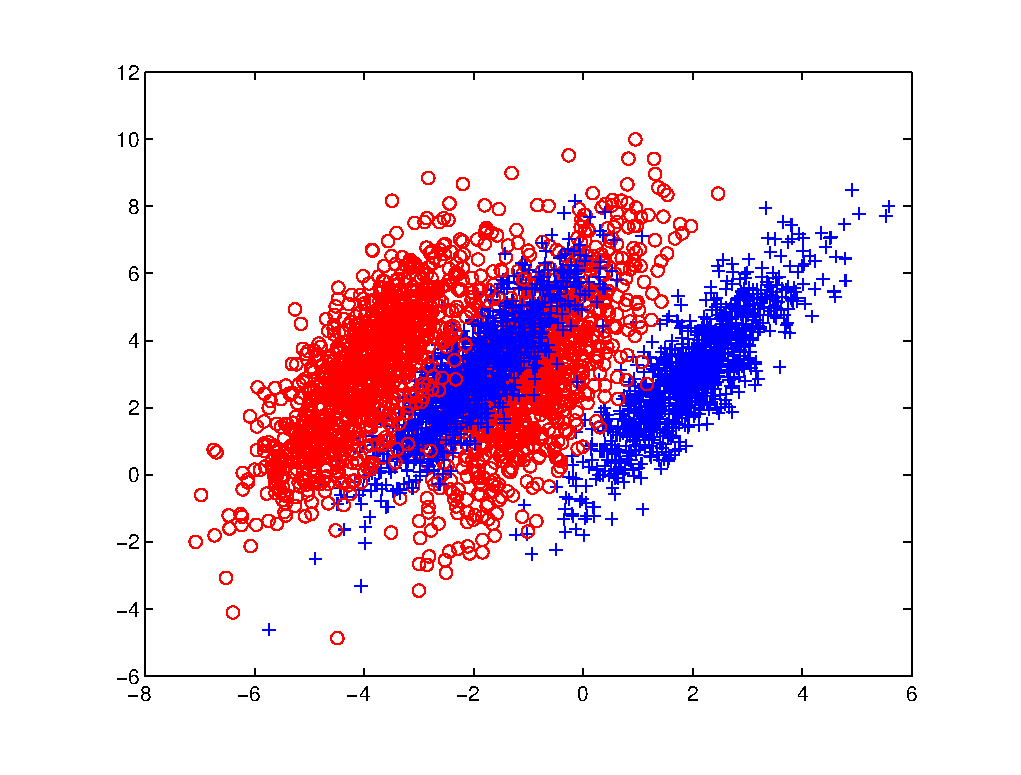
\includegraphics[width=2cm]{3_review/figures/classification/pbt-simulation/pbt_tree_1.eps}}; 
    \edge node[auto=right] {};
    [.\node{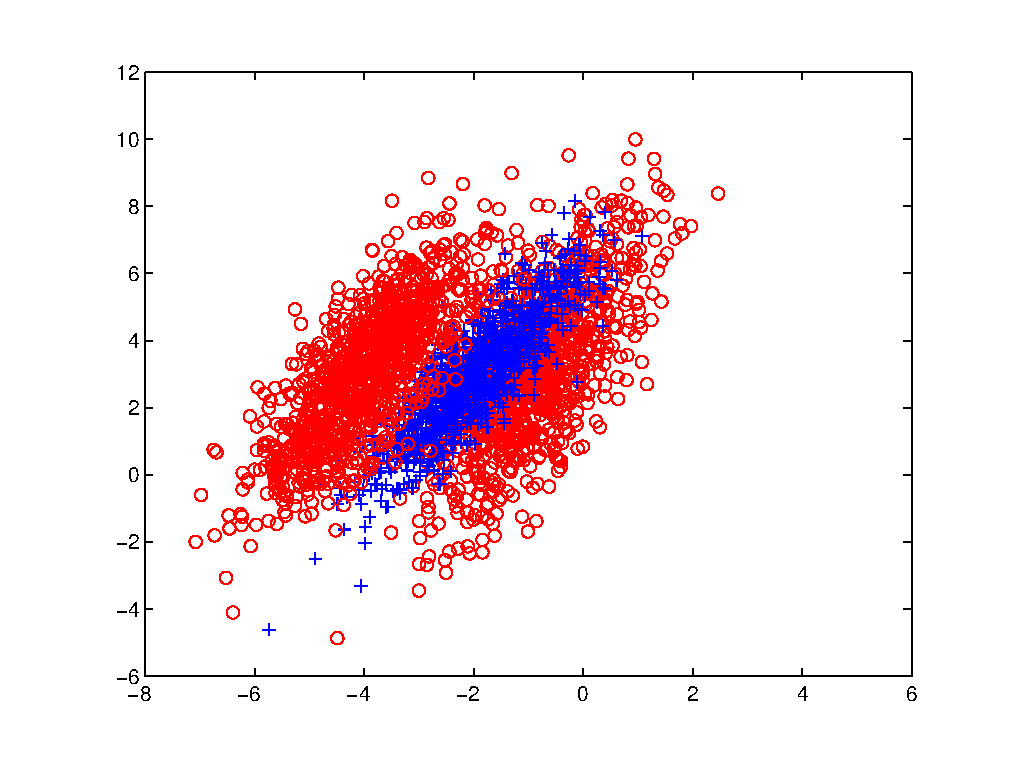
\includegraphics[width=2cm]{3_review/figures/classification/pbt-simulation/pbt_tree_2_1.eps}};
      \edge node[auto=right] {};  
      [.\node{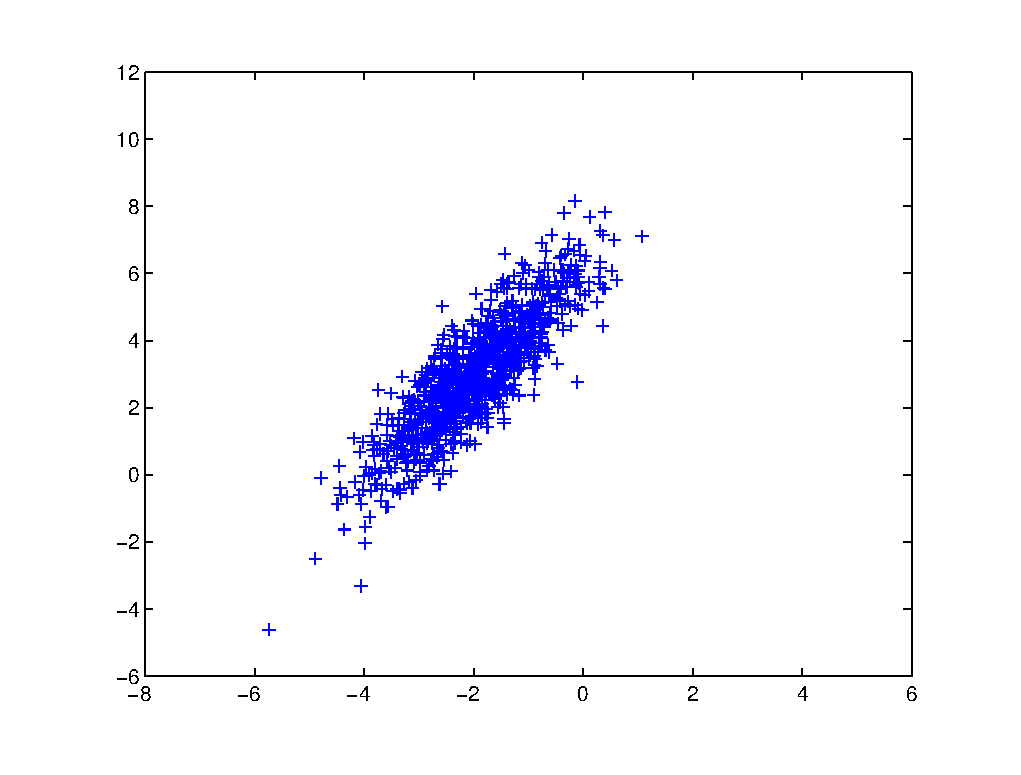
\includegraphics[width=2cm]{3_review/figures/classification/pbt-simulation/pbt_tree_3_2.eps}}; ]
      \edge node[auto=left] {};  
      [.\node{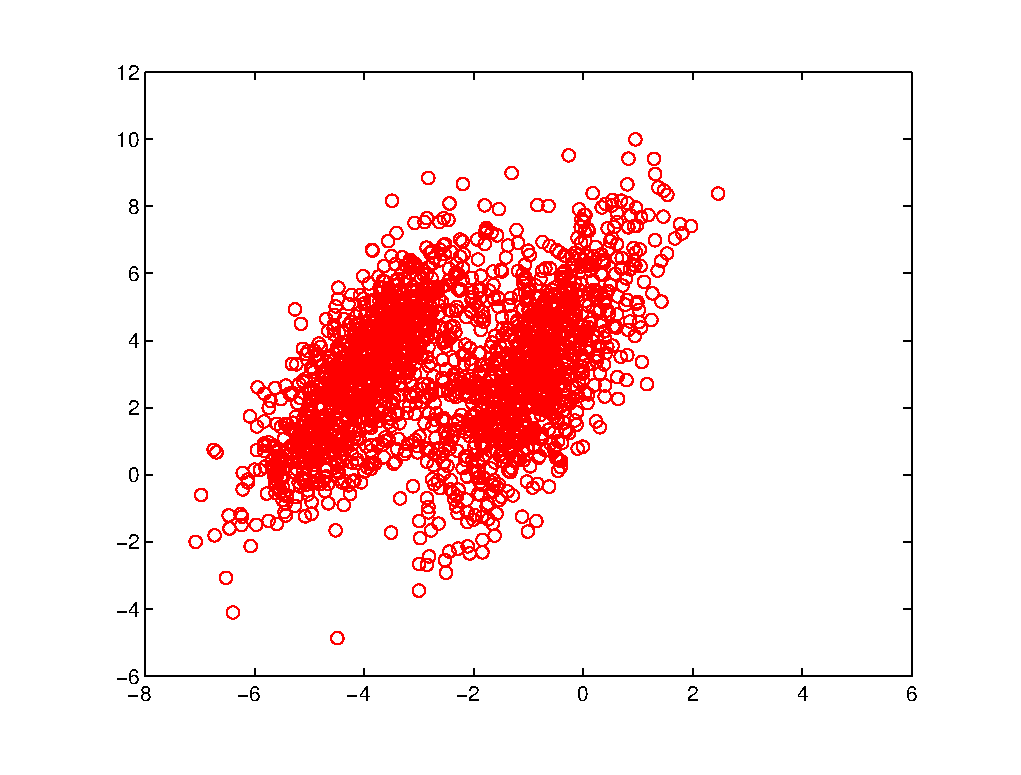
\includegraphics[width=2cm]{3_review/figures/classification/pbt-simulation/pbt_tree_3_1.eps}}; ]
    ]
    \edge node[auto=left] {};
    [.\node{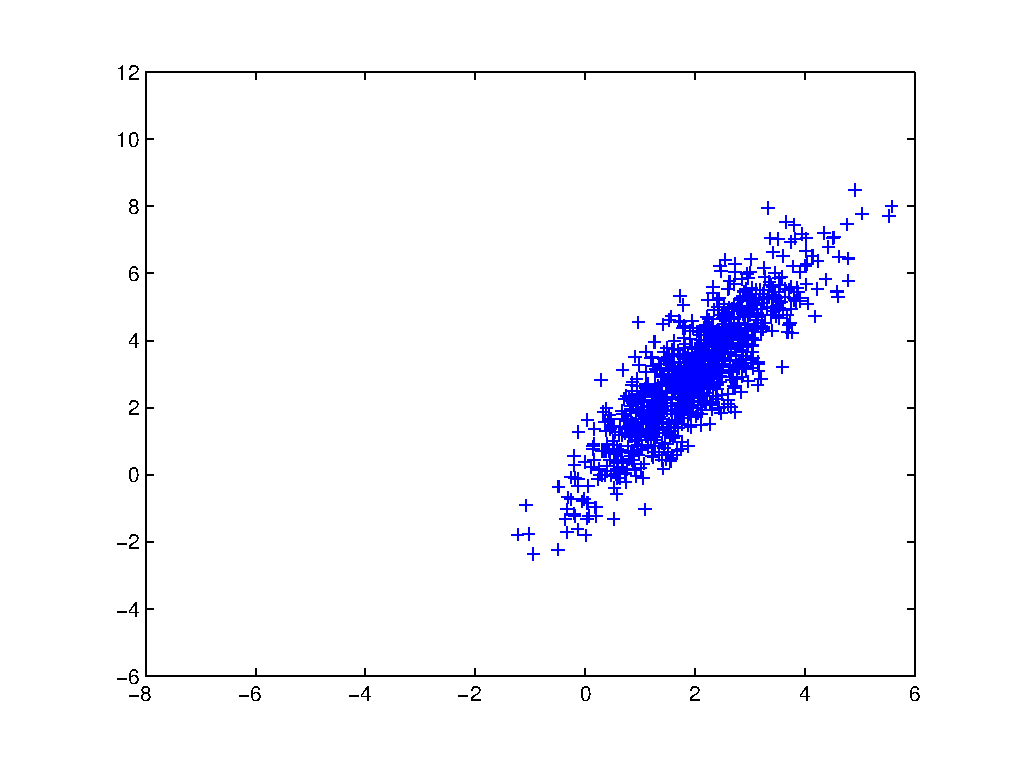
\includegraphics[width=2cm]{3_review/figures/classification/pbt-simulation/pbt_tree_2_2.eps}};
    ]
    ];
	\end{tikzpicture}
\caption[Representation of the probabilistic boosting-tree.]{Representation of the capabilities of the probabilistic boosting-tree algorithm to split at each node of the tree the positive and negative samples.}
\label{fig:pbtsim}
\end{figure}

Probabilistic boosting-tree is another ensemble learning classifier which shares principles with AdaBoost but using them inside a decision tree~\cite{Tu2005}. 
In the training stage, the probabilistic boosting-tree method grows a decision tree and at each node, a strong classifier is learned in an almost comparable scheme to AdaBoost.
Once the strong learner is trained, the training set is split into two subsets which are used to train the next strong classifiers in the next descending nodes.
Thus, three cases are conceivable to decide in which branch to propagate each sample training $\mathbf{x}_i$:

\begin{itemize}
	\item if $q(+1, \mathbf{x}_i) - \frac{1}{2} > \epsilon$ then $\mathbf{x}_i$ is propagated to the right branch set and a weight $w_i=1$ is assigned. 
	\item if $q(-1, \mathbf{x}_i) - \frac{1}{2} > \epsilon$ then $\mathbf{x}_i$ is propagated to the left branch set and a weight $w_i=1$ is assigned.
	\item else $\mathbf{x}_i$ will be propagated in both branches with $w_i=q(+1, \mathbf{x}_i)$ in the right branch and $w_i=q(-1, \mathbf{x}_i)$ in the left branch.
\end{itemize}

\noindent with $\mathbf{w} = w_i, i=\{1,\cdots,N\}$ corresponding to distribution of weights, $N$ the number of samples as in AdaBoost and $q(\cdot)$ is defined as:

\begin{eqnarray}
	q(+1, \mathbf{x}_i) & = & \frac{\exp(2H(\mathbf{x}_i))}{1+\exp(2H(\mathbf{x}_i))} \ , \label{eq:regada1} \\
	q(-1, \mathbf{x}_i) & = & \frac{\exp(-2H(\mathbf{x}_i))}{1+\exp(-2H(\mathbf{x}_i))} \ . \label{eq:regada2}
\end{eqnarray}

Employing such a scheme tends to divide the data in such a way that positive and negative samples are naturally split as shown in \acs{eq}\,\ref{fig:pbtsim}.
In the classification stage, the unlabelled sample $\mathbf{x}$ is propagated through the tree, where at each node, it is classified by each strong classifier previously learned and where an estimation of the posterior distribution is computed.
The posterior distribution corresponds to the sum of the posterior distribution at each node of the decision tree.
The probabilistic boosting-tree classifier has been used in~\cite{Tiwari2009a,Tiwari2012,Tiwari2010,Viswanath2011}.

\paragraph{Kernel method}
A Gaussian process for classification is a kernel method in which it is assumed that the data can be represented by a single sample from a multivariate Gaussian distribution~\cite{Rasmussen2005}.
In the case of linear logistic regression for classification, the posterior probability is expressed as:
\begin{eqnarray}
	p(y_i|\mathbf{x}_i,\mathbf{w}) & = & \sigma(y_i f(\mathbf{x}_i)) \ , \label{eq:gp1} \\
	f(\mathbf{x}_i) & = & \mathbf{x}_i^{\text{T}} \mathbf{w} \ , \nonumber
\end{eqnarray}

\noindent where $\sigma(\cdot)$ is the logistic function and $\mathbf{w}$ are the parameters vector of the model.
Thus, the classification using Gaussian processes is based on assigning a Gaussian process prior over the function $f(\mathbf{x})$ which is characterized by a mean function $\bar{f}$ and covariance function $K$.
Therefore, in the training stage, the best mean and covariance functions have to be inferred in regard to our training data using a Newton optimization and a Laplacian approximation.
The prediction stage is performed in two stages.
First, for a new observation $\mathbf{x}_*$, the corresponding probability $p(f(\mathbf{x}_*)|f(\mathbf{x}))$ is computed such that:
\begin{eqnarray}
	p(f(\mathbf{x}_*)|f(\mathbf{x})) & = & \mathcal{N}( K_*K^{-1}\bar{f}, K_{**}-K_*(K')^{-1}K_*^{\text{T}} ) \ , \nonumber \\
	K' & = & K + W^{-1} \ , \label{eq:gp2} \\
	W & = & \nabla \nabla \log p(\mathbf{y}|f(\mathbf{x})) \ , \nonumber
\end{eqnarray}

\noindent where $K_{**}$ is the covariance function $k(\mathbf{x}_*, \mathbf{x}_*)$ the testing sample $\mathbf{x}_*$, $K_{*}$ is the covariance function $k(\mathbf{x}, \mathbf{x}_*)$ of training-testing samples $\mathbf{x}$ and $\mathbf{x}_*$.
Then, the function $f(\mathbf{x}_*)$ is squashed using the sigmoid function and the probability of the class membership is defined such that:

\begin{equation}
	C(\mathbf{x}_*) = \sigma\left( \frac{\bar{f}(\mathbf{x_*})}{\sqrt{1+var(f(\mathbf{x}_*))}} \right) \ .
	\label{eq:gp3}
\end{equation}

Only \citeauthor{Kelm2007} used Gaussian process for classification of \ac{mrsi} data~\cite{Kelm2007}.

\paragraph{Sparse kernel methods}
In a classification scheme using Gaussian processes, when a prediction is performed, the whole training data are used to assign a label to the new observations.
That is why this method is also called kernel method.
Sparse kernel category is composed of methods which rely only on a few labelled observations of the training set to assign the label of new observations~\cite{Bishop2006}.

\Acf{svm} is a sparse kernel method aiming at finding the best linear hyper-plane --- non-linear separation is discussed further --- which separates 2 classes such that the margin between the two classes is maximized~\cite{Vapnik1963}.
The margin is in fact the region defined by 2 hyper-planes splitting the 2 classes, such that there is no points lying in between.
The distance between these 2 hyper-planes is equal to $\frac{2}{\|\mathbf{w}\|}$ where $\mathbf{w}$ is the normal vector of the hyper-plane splitting the classes.
Thus, maximizing the margin is equivalent to minimizing the norm $\|\mathbf{w}\|$.
Hence, this problem is solved by an optimization approach and formalized as:

\begin{equation}
\begin{aligned}
& \argmin_{\mathbf{w}}
& & \frac{1}{2} \| \mathbf{w}^2\| \ , \\
& \text{subject to}
& & y_i(\mathbf{w}.\mathbf{x}_i - b) \geq 1, \; i = \{ 1, \ldots, N \} \ ,
\end{aligned}
\label{eq:svm1}
\end{equation}

\noindent where $\mathbf{x}_i$ is a training sample with is corresponding class label $y_i$.
From \acs{eq}\,\eqref{eq:svm1}, it is important to notice that only few points from the set of $N$ points are selected which later define the hyper-plane.
This constraint is imposed in the optimization problem using Lagrange multipliers $\boldsymbol{\alpha}$.
All points which are not lying on the margin are assigned a corresponding $\alpha_i = 0$, which is formalized as \acs{eq}\,\eqref{eq:svm2}.

\begin{equation}
	\arg\min_{\mathbf{w},b } \max_{\boldsymbol{\alpha}\geq 0 } \left\{ \frac{1}{2}\|\mathbf{w}\|^2 - \sum_{i=1}^{n}{\alpha_i[y_i(\mathbf{w}\cdot \mathbf{x_i} - b)-1]} \right\} \ .
	\label{eq:svm2}
\end{equation}

The different parameters are inferred using quadratic programming.
This version of \ac{svm} is known as hard-margin since no points can lie in the margin area.
However, it is highly probable not to find any hyper-plane splitting the classes such as specified previously.
Thus, a soft-margin optimization approach has been proposed~\cite{Cortes1995}, where points have the possibility to lie on the margin but at the cost of a penalty $\xi_i$ which is minimized in the optimization process such that:

\begin{equation}
\small
\arg\min_{\mathbf{w},\mathbf{\xi}, b } \max_{\boldsymbol{\alpha},\boldsymbol{\beta} } \left\{ \frac{1}{2}\|\mathbf{w}\|^2+C \sum_{i=1}^n \xi_i - \sum_{i=1}^{n}{\alpha_i[y_i(\mathbf{w}\cdot \mathbf{x_i} - b) -1 + \xi_i]} - \sum_{i=1}^{n} \beta_i \xi_i \right\} \ .
\end{equation}

The decision to assign the label to a new observation $\mathbf{x}_i$ is taken such that:

\begin{equation}
	C(\mathbf{x}_i) = \sign \left( \sum_{n=1}^{N} \alpha_n (\mathbf{x}_n . \mathbf{x}_i) + b_0 \right) \ ,
	\label{eq:svmdec} 
\end{equation}

\noindent where $\mathbf{x}_n|n=\{1,\cdots,S\}$, $S$ being the support vectors.

\ac{svm} can also be used as a non-linear classifier by performing a Kernel trick~\cite{Boser1992}.
The original data $\mathbf{x}$ is projected to a high-dimensional space in which it is assumed that a linear hyper-plane splits the 2 classes.
Different kernels are popular such as the \ac{rbf} kernel, polynomial kernels, or sigmoid kernels.
In \ac{cad} for \ac{cap} systems, \ac{svm} is the most popular classification method and has been used in a multitude of research works~\cite{Artan2009,Artan2010,Chan2003,Litjens2011,Litjens2012,Liu2013,Lopes2011,Niaf2011,Niaf2012,Ozer2009,Ozer2010,Parfait2012,Peng2013,Sung2011,Tiwari2012,Vos2008,Vos2008a,Vos2010,Vos2012,giannini2015fully,trigui2017automatic,lehaire2014computer,khalvati2015automated,chung2015prostate}.

\Acf{rvm} is a sparse version of Gaussian process previously presented, proposed in~\cite{Tipping2001}.
\ac{rvm} is identical to a Gaussian process with the following covariance function~\cite{Quinonero-Candela2002}:

\begin{equation}
	K_{RVM}(\mathbf{x}_p,\mathbf{x}_q) = \sum_{j=1}^{M} \frac{1}{\alpha_j} \Phi_j ( \mathbf{x}_p ) \Phi_j ( \mathbf{x}_q ) \ ,
 	\label{eq:rvm}
\end{equation}

\noindent where $\phi(\cdot)$ is a Gaussian basis function, $\mathbf{x}_i|i=\{1,\cdots,N\}$ are the $N$ training points, and $\boldsymbol{\alpha}$ are the weights vector.
As mentioned in~\cite{Quinonero-Candela2002}, the sparsity regarding the relevance vector arises for some $j$, the weight $\alpha_j^{-1} = 0$.
The set of weights $\boldsymbol{\alpha}$ is inferred using the expectation maximization algorithm.
\citeauthor{Ozer2010} used of \ac{rvm} and make a comparison with \ac{svm} for the task of \ac{cap} detection~\cite{Ozer2009,Ozer2010}.

\paragraph{Neural network} 
Multilayer perceptron is a feed-forward neural network considered as the most successful model of this kind in pattern recognition~\cite{Bishop2006}.
The most well known model used is based on 2 layers where a prediction of an observation is computed as:

\begin{equation}
	C(\mathbf{x}_n,w_{ij}^{(1)},w_{kj}^{(2)}) = \sigma \left[ \sum_{j=0}^{M} w_{kj}^{(2)} \  h \left( \sum_{i=0}^{D} w_{ij}^{(1)} x_{in} \right) \right] \ ,
	\label{eq:annmlp}
\end{equation}

\noindent where $h(\cdot)$ and $\sigma(\cdot)$ are 2 activation functions usually non-linear, $w_{ij}^{(1)}$ and $ w_{kj}^{(2)}$ are the weights associated with the linear combination with the input feature $\mathbf{x}_n$ and the hidden unit.

\begin{figure}
\centering
\def\layersep{3cm}
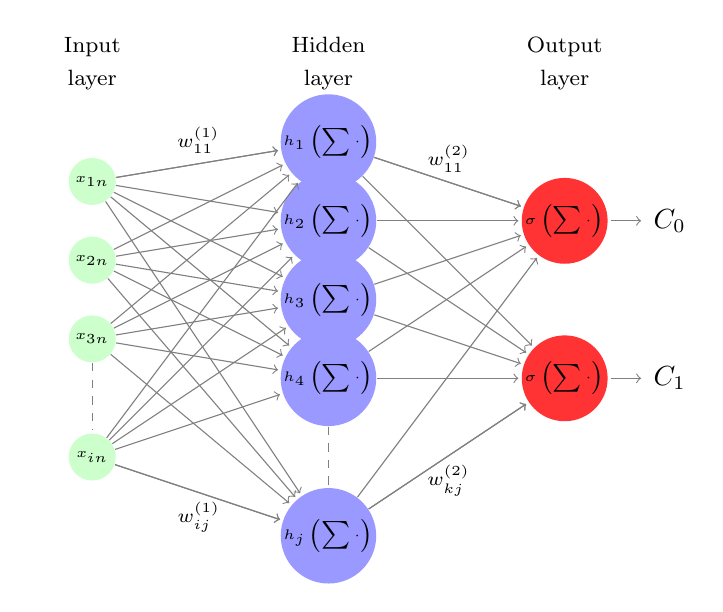
\begin{tikzpicture}[shorten >=1pt,draw=black!50, node distance=\layersep]
    \tikzstyle{every pin edge}=[<-,shorten <=1pt]
    \tikzstyle{neuron}=[circle,fill=black!25,minimum size=17pt,inner sep=0pt]
    \tikzstyle{input neuron}=[neuron, fill=green!20];
    \tikzstyle{output neuron}=[neuron, fill=red!80];
    \tikzstyle{hidden neuron}=[neuron, fill=blue!40];
    \tikzstyle{annot} = [text width=4em, text centered]

    % Draw the input layer nodes
    \foreach \name / \y in {1,...,3}
    % This is the same as writing \foreach \name / \y in {1/1,2/2,3/3,4/4}
        \node[input neuron] (I-\name) at (0,-\y) {\tiny $x_{ \y n }$};
        
   \node[input neuron] (I-4) at (0,-4.5) {\tiny $x_{in}$};
   \draw[dashed,draw=black!50] (I-3) -- (I-4);

    % Draw the hidden layer nodes
    \foreach \name / \y in {1,...,4}
        \path[yshift=0.5cm]
            node[hidden neuron] (H-\name) at (\layersep,-\y cm) {\tiny $h_{ \y }\left(\sum \cdot \right)$};
            
    \node[hidden neuron] (H-5) at (\layersep,-5.5 cm) {\tiny $h_{j}\left(\sum \cdot \right)$};
    \draw[dashed,draw=black!50] (H-4) -- (H-5);

    % Draw the output layer node
    	\node[output neuron,pin={[pin edge={->}]right:$C_{0}$}, right of=H-2] (O-1) {\tiny $\sigma\left(\sum \cdot \right)$};
    	\node[output neuron,pin={[pin edge={->}]right:$C_{1}$}, right of=H-4] (O-2) {\tiny $\sigma\left(\sum \cdot \right)$};

    % Connect every node in the input layer with every node in the
    % hidden layer.
    \foreach \source in {1,...,4}
        \foreach \dest in {1,...,5}
        		\draw[shorten >=1pt,->,draw=black!50] (I-\source)  -- (H-\dest);
            %\path (I-\source) edge (H-\dest);
    
    % Draw the annotation for the weight for the first and last connections       
    \draw[shorten >=1pt,->,draw=black!50] (I-1) -- (H-1) node [midway, above] (w111) {\scriptsize $w_{11}^{(1)}$};
    \draw[shorten >=1pt,->,draw=black!50] (I-4) -- (H-5) node [midway, below] (w145) {\scriptsize $w_{ij}^{(1)}$};

    % Connect every node in the hidden layer with the output layer
    \foreach \source in {1,...,5}
    		\foreach \dest in {1,...,2}
        		\draw[shorten >=1pt,->,draw=black!50] (H-\source)  -- (O-\dest);
        %\path (H-\source) edge (O);
        
    % Draw the annotation for the weight for the first and last connections       
    \draw[shorten >=1pt,->,draw=black!50] (H-1) -- (O-1) node [midway, above] (w211) {\scriptsize $w_{11}^{(2)}$};
    \draw[shorten >=1pt,->,draw=black!50] (H-5) -- (O-2) node [midway, below] (w251) {\scriptsize $w_{kj}^{(2)}$};

    % Annotate the layers
    \node[annot,above of=H-1, node distance=1cm] (hl) {\footnotesize Hidden layer};
    \node[annot,left of=hl] {\footnotesize Input layer};
    \node[annot,right of=hl] {\footnotesize Output layer};
\end{tikzpicture}
\caption{Representation of a neural network of the multilayer perceptron family.}
\label{fig:mlp}
\end{figure}


A graphical representation of this network is presented in \acs{eq}\,\ref{fig:mlp}.
Relating \acs{fig}\,\ref{fig:mlp} with \acs{eq}\,\eqref{eq:annmlp}, it can be noted that this network is composed of some successive non-linear mapping of the input data.
First, a linear combination of the input vector $\mathbf{x}_n$ is mapped into some hidden units through a set of weights $w_{ij}^{(1)}$.
This combination becomes non-linear by the use of the activation function $h(\cdot)$ which is usually chosen to be a sigmoid function.
Then, the output of the networks consists of a linear combination of the hidden units and the set of weights $w_{kj}^{(2)}$.
This combination is also mapped non-linearly using an activation function $\sigma(\cdot)$ which is usually a logistic function.
Thus, the training of such a network resides in finding the best weights $w_{ij}^{(1)}$ and $ w_{kj}^{(2)}$ which model the best the training data.
The error of this model is computed as:

\begin{equation}
	E(w_{ij}^{(1)},w_{kj}^{(2)}) = \frac{1}{2} \sum_{n=1}^{N} \left( C(\mathbf{x}_n,w_{ij}^{(1)},w_{kj}^{(2)}) - y(\mathbf{x}_n) \right) ^{2} \ ,
	\label{eq:mlpcost}
\end{equation}

\noindent where $\mathbf{x}_n|n=\{1,\cdots,N\}$ are the $N$ training vectors with their corresponding class label $y(\mathbf{x}_n)$.

Therefore, the best set of weights is inferred in an optimization framework where the error $E(\cdot)$ needs to be minimized.
This optimization is performed using a gradient descent method where the derivative of \acs{eq}\,\eqref{eq:mlpcost} is computed using the back-propagation algorithm proposed by~\cite{Rumelhart1988}.
This type of network has been used multiple times~\cite{Matulewicz2013,Parfait2012,trigui2017automatic,trigui2016classification,rampun2016computer}.

\begin{figure}
\centering
\def\layersep{3cm}
\def\finallayersep{2.2cm}
\begin{tikzpicture}[shorten >=1pt,draw=black!50, node distance=\layersep]
    \tikzstyle{every pin edge}=[<-,shorten <=1pt]
    \tikzstyle{neuron}=[circle,fill=black!25,minimum size=20pt,inner sep=0pt]
    \tikzstyle{input neuron}=[neuron, fill=green!20];
    \tikzstyle{output neuron}=[neuron, fill=red!80];
    \tikzstyle{hidden neuron}=[neuron, fill=blue!20];
    \tikzstyle{summation neuron}=[neuron, fill=blue!40];
    \tikzstyle{annot} = [text width=4em, text centered]

    % Draw the input layer nodes
    \foreach \name / \y in {1,...,3}
    % This is the same as writing \foreach \name / \y in {1/1,2/2,3/3,4/4}
        \node[input neuron] (I-\name) at (0,-\y-1) {\tiny $x_{ \y n }$};
        
   \node[input neuron] (I-4) at (0,-5.5) {\tiny $x_{in}$};
   \draw[dashed,draw=black!50] (I-3) -- (I-4);
   
   % Draw the pattern layer
   \node[hidden neuron] (H-1) at (\layersep,0 cm) {\tiny $h_{11}\left( \cdot \right)$};
   \node[hidden neuron] (H-2) at (\layersep,-1 cm) {\tiny $h_{21}\left( \cdot \right)$};
   \node[hidden neuron] (H-3) at (\layersep,-2.5 cm) {\tiny $h_{31}\left( \cdot \right)$};
   \draw[dashed,draw=black!50] (H-2) -- (H-3);
   
   \begin{pgfonlayer}{background}
	\path (H-1.west |- H-1.north)+(-0.2,0.2) node (a) {};
    \path (H-3.east |- H-3.south)+(+0.2,-0.2) node (b) {};
          
    \path[fill=blue!10,rounded corners, draw=blue!50, dashed] (a) rectangle (b);
   \end{pgfonlayer}
   
   \node[hidden neuron] (H-4) at (\layersep,-4.5 cm) {\tiny $h_{12}\left( \cdot \right)$};
   \node[hidden neuron] (H-5) at (\layersep,-5.5 cm) {\tiny $h_{22}\left( \cdot \right)$};
   \node[hidden neuron] (H-6) at (\layersep,-7 cm) {\tiny $h_{32}\left( \cdot \right)$};
   \draw[dashed,draw=black!50] (H-5) -- (H-6);
   
   \begin{pgfonlayer}{background}
	\path (H-4.west |- H-4.north)+(-0.2,0.2) node (c) {};
    \path (H-6.east |- H-6.south)+(+0.2,-0.2) node (d) {};
          
    \path[fill=blue!10,rounded corners, draw=blue!50, dashed] (c) rectangle (d);
   \end{pgfonlayer}
   
   % Draw the summation layer
   \begin{scope}[node distance=2cm]
   \node[summation neuron, right of=H-2] (S-1) {\tiny $\sum_1 \cdot $};
   \node[summation neuron, right of=H-5] (S-2) {\tiny $\sum_2 \cdot $};
   \end{scope}
   
   % Draw the decision layer
   \node[output neuron,pin={[pin edge={->}]right:$C$},] at (3*\finallayersep,-3.5 cm) (O) {$\sigma \left( \cdot \right)$};
   
   % Draw the networking from input layer to pattern layer
   \foreach \source in {1,...,4}
   		\foreach \dest in {1,...,6}
   				\draw[shorten >=1pt,->,draw=black!50] (I-\source)  -- (H-\dest);
   				
   % Draw the networking from pattern layer to summation layer
   \foreach \source in {1,...,3}
   		\draw[shorten >=1pt,->,draw=black!50] (H-\source)  -- (S-1);
   		
   	\foreach \source in {4,...,6}
   		\draw[shorten >=1pt,->,draw=black!50] (H-\source)  -- (S-2);
   		
   	% Draw from summation layer to ouput
   	\draw[shorten >=1pt,->,draw=black!50] (S-1)  -- (O);
   	\draw[shorten >=1pt,->,draw=black!50] (S-2)  -- (O);
  
    % Annotate the layers
    \node[annot,above of=H-1, node distance=1cm] (hl) {\footnotesize Pattern layer};
    \node[annot,left of=hl] {\footnotesize Input layer};
    \begin{scope}[node distance=2cm]
    \node[annot,right of=hl] {\footnotesize Summation layer};
    \end{scope}
    \node[annot,above of=O, node distance=4.5cm] (o) {\footnotesize Decision layer};
\end{tikzpicture}
\caption{Representation of a neural network of the probabilistic neural network family.}
\label{fig:pnn}
\end{figure}


Probabilistic neural networks are another type of feed-forward networks which is derived from the multilayer perceptron case and has been proposed by~\cite{Specht1988}.
This classifier is modelled by changing the activation function $h(\cdot)$ in \acs{eq}\,\eqref{eq:annmlp} to an exponential function such that:

\begin{equation}
	h(\mathbf{x}_n) = \exp \left( - \frac{ (\mathbf{w}_j - \mathbf{x})^{\text{T}}(\mathbf{w}_j - \mathbf{x}) }{2\sigma^2} \right) \ ,
	\label{eq:pnn1}
\end{equation}

\noindent where $\sigma$ is a free parameter set by the user.

The other difference of the probabilistic neural networks compared with the multilayer perceptron networks resides in the architecture as shown in \acs{fig}\,\ref{fig:pnn}.
This network is formed by 2 hidden layers.
The first hidden layer consists of the pattern layer, in which the mapping is done using \acs{eq}\,\eqref{eq:pnn1}.
This pattern layer is sub-divided into a number of groups corresponding to the number of classes.
The second hidden layer corresponds to the summation layer which simply sums the output of each sub-group of the pattern layer.
This method is used in~\cite{Ampeliotis2007,Ampeliotis2008,Viswanath2011}.

\paragraph{Graphical model classifiers}
\Ac{mrf} is used as a lesion segmentation method to detect \ac{cap}.
First, let define $s$ as a pixel which belongs to a certain class denoted by $\omega_s$.
The labelling process is defined as $\omega = \{\omega_s, s \in I\}$ where $I$ is the set of all the pixels inside the image.
The observations corresponding to \ac{si} in the image are noted $\mathcal{F} = \{ f_s | s \in I \}$.
Thus, the image process $\mathcal{F}$ represents the deviation from the labelling process $\omega$~\cite{Kato2001}.
Hence, lesion segmentation is equivalent to estimating the best $\hat{\omega}$ which maximizes the posterior probability $p(\omega|\mathcal{F})$.
Thus, using a Bayesian approach, this problem is formulated such that:

\begin{equation}
	p(\omega|\mathcal{F}) = \argmax_{\omega} \prod_{s \in I} p(f_s | \omega_s) p(\omega) \ .
	\label{eq:mrf1}
\end{equation}

It is generally assumed that $p(f_s | \omega_s)$ follows a Gaussian distribution and that the pixels classes $\lambda = \{1,2\}$ for a binary classification are characterized by their respective mean $\mu_{\lambda}$ and standard deviation $\sigma_{\lambda}$.
Then, $\omega$ is a Markov random field, thus:

\begin{equation}
	p(\omega) =  \frac{1}{Z} \exp\left( -U(\omega) \right)  \ ,
	\label{eq:mrf2}
\end{equation}

\noindent where $Z$ is a normalization factor to obtain a probability value, $U(\cdot)$ is the energy function.

Thus, the segmentation problem is solved as an optimization problem where the energy function $U(\cdot)$ has to be minimized.
There are different possibilities to define the energy function $U(\cdot)$.
However, it is common to define the energy function such that it combines two types of potential function: (i) a local term relative to the pixel itself and (ii) a smoothing prior which embeds neighbourhood information which penalizes the energy function affecting the region homogeneity.
This optimization of such a function can be performed using an algorithm such as iterated conditional modes~\cite{Kato2001}.
\citeauthor{Liu2009} and \citeauthor{Ozer2010} used \ac{mrf} as an unsupervised method to segment lesions in \ac{mpmri} images~\cite{Liu2009,Ozer2010}.
\citeauthor{Artan2010} and \citeauthor{chung2015prostate} used conditional random fields instead of \ac{mrf} for \ac{mri} segmentation~\cite{Artan2009,Artan2010,chung2015prostate}.
The difference between these 2 methods resides in the fact that conditional probabilities are defined such as:

\begin{equation}
	p(\omega|\mathcal{F}) =  \frac{1}{Z} \exp \left[ - \sum_{s \in I} V_{C1}(\omega_s|\mathcal{F}) - \sum_{\{s,r\} \in C } V_{C2} (\omega_s,\omega_r|\mathcal{F})  \right] \ .
\label{eq:crf}
\end{equation}

\noindent $V_{C1}(\cdot)$ is the state (or partition) feature function and $V_{C2}(\cdot)$ is the transition (or edge) feature function~\cite{Kato2012}.

\subsubsection{Summary}

Classification methods used to distinguish \ac{cap} from healthy tissue in in \ac{cad} systems are summarized in \acs{tab}~\ref{tab:class}.

\begin{table}
  \caption{Overview of the classifiers used in \acs*{cad} systems.}
  \scriptsize
  \begin{tabularx}{\textwidth}{l >{\raggedleft\arraybackslash}X@{}}
    \toprule
    \textbf{Classifier} & \textbf{References} \\
    \midrule
    \textbf{Rule-based method:} & \cite{Lv2009,Puech2009} \\ \\ [-1.5ex]
    \textbf{Clustering methods:} & \\
    \quad $k$-means clustering & \cite{Tiwari2007,Tiwari2008,Tiwari2009} \\
    \quad \acs{knn} & \cite{Litjens2012,Niaf2011,Niaf2012,rampun2016computerb} \\ \\ [-1.5ex]
    \textbf{Linear model classifiers:} & \\
    \quad \acs{lda} & \cite{Antic2013,Chan2003,Litjens2014,Niaf2011,Niaf2012,Vos2012} \\
    \quad Logistic regression & \cite{Kelm2007,Langer2009,lehaire2014computer,rampun2015computer} \\ \\ [-1.5ex]
    \textbf{Non-linear classifier:} & \\
    \quad \acs{qda} & \cite{Viswanath2012} \\ \\ [-1.5ex]
    \textbf{Probabilistic classifier:} & \\
    \quad Naive Bayes & \cite{Giannini2013,Mazzetti2011,Niaf2011,Niaf2012,cameron2014multiparametric,cameron2016maps,rampun2015classifying,rampun2016computerb,rampun2015computer,rampun2016computer} \\ \\ [-1.5ex]
    \textbf{Ensemble learning classifiers:} & \\
    \quad AdaBoost & \cite{Litjens2014,Lopes2011} \\
    \quad \acs*{rf} & \cite{Kelm2007,Litjens2014,Tiwari2012,Tiwari2013,Viswanath2009,trigui2017automatic,trigui2016classification,samarasinghe2016semi,rampun2015classifying,rampun2016computerb,rampun2015computer,rampun2016computer} \\
    \quad Probabilistic boosting tree & \cite{Tiwari2009,Tiwari2010,Tiwari2012} \\ \\ [-1.5ex]
    \textbf{Kernel method:} & \\
    \quad Gaussian processes & \cite{Kelm2007} \\ \\ [-1.5ex]
    \textbf{Sparse kernel methods:} & \\
    \quad \acs{svm} & \cite{Artan2009,Artan2010,Chan2003,Litjens2011,Litjens2012,Liu2013,Lopes2011,Niaf2011,Niaf2012,Ozer2009,Ozer2010,Parfait2012,Peng2013,Sung2011,Tiwari2012,Vos2008,Vos2008a,Vos2010,Vos2012,giannini2015fully,trigui2017automatic,lehaire2014computer,khalvati2015automated,chung2015prostate} \\
    \quad \acs{rvm} & \cite{Ozer2009,Ozer2010} \\ \\ [-1.5ex]
    \textbf{Neural network:} & \\ 
    \quad Multiple layer perceptron & \cite{Matulewicz2013,Parfait2012,trigui2017automatic,trigui2016classification,rampun2016computer} \\
    \quad Probabilistic neural network & \cite{Ampeliotis2007,Ampeliotis2008,Viswanath2011} \\ \\ [-1.5ex]
    \textbf{Graphical model classifiers:} & \\
    \quad Markov random field & \cite{Liu2009,Ozer2010} \\
    \quad Conditional random field & \cite{Artan2009,Artan2010,chung2015prostate} \\
    \bottomrule
  \end{tabularx}
\label{tab:class}
\end{table}

\subsection{Model validation} \label{subsec:chp3:img-clas:CADX-val}

\begin{table}
  \caption{Overview of the model validation techniques used in \acs*{cad} systems.}
  \centering
  \scriptsize
  % \renewcommand{\arraystretch}{1.5}
  \begin{tabularx}{\textwidth}{@{}l >{\raggedleft\arraybackslash}X@{}}
    \toprule
    \textbf{Model validation techniques} & \textbf{References} \\ \\ [-1.5ex]
    \midrule
    \quad \acs*{loo} & \cite{Ampeliotis2007,Ampeliotis2008,Antic2013,Artan2009,Artan2010,Chan2003,Giannini2013,Kelm2007,Litjens2012,Litjens2014,Mazzetti2011,Niaf2011,Niaf2012,Ozer2009,Ozer2010,Peng2013,Puech2009,Tiwari2013,Viswanath2011,Vos2008,Vos2008,Vos2010,cameron2016maps,cameron2014multiparametric,lehaire2014computer,khalvati2015automated,chung2015prostate} \\ \\ [-1.5ex]
    \quad \acs*{kcv} & \cite{Litjens2011,Parfait2012,Tiwari2009,Tiwari2009a,Tiwari2010,Tiwari2012,Viswanath2012,Viswanath2009,Vos2012,trigui2016classification,trigui2017automatic,rampun2015classifying,rampun2015computer,rampun2016computer,rampun2016computerb,rampun2016quantitative} \\ \\ [-1.5ex]
    \bottomrule
  \end{tabularx}
\label{tab:valmod}
\end{table}

In pattern recognition, the use of model validation techniques to assess the performance of a classifier plays an important role for reporting results.
Two techniques are broadly used in the development of \ac{cad} systems and are summarized in \acs{tab}~\ref{tab:valmod}.
The most popular technique used in \ac{cad} systems is the \acf{loo} technique.
From the whole data, one patient is kept for validation and the other cases are used for training.
This manipulation is repeated until each patient has been used for validation.
This technique is popular when working with a limited number of patients, allowing to train on representative number of cases even with a small dataset.
However, \ac{loo} cross-validation suffers from a large variance and is considered as an unreliable estimate~\cite{Efron1983}.

The other technique is the \acf{kcv} technique which is based on splitting the dataset into $k$ subsets where the samples are randomly selected.
Then, one fold is kept for testing and the remaining subsets are used for training.
The classification is then repeated as in the \ac{loo} technique.
In fact \acf{loo} is a particular case of \acf{kcv} when $k$ equals the number of patients.
In the reviewed papers, the typical values used for $k$ has been set to three and five.
\acf{kcv} is regarded as more appropriate than \acf{loo}, but the number of patients in the dataset needs to be large enough for the results to be meaningful.

\subsection{Evaluation measures} \label{subsec:chp3:img-clas:eval-mea}

\begin{table}
  \caption{Overview of the evaluation metrics used in \acs*{cad} systems.}
  \scriptsize
  \begin{tabularx}{\textwidth}{@{}l >{\raggedleft\arraybackslash}X@{}}
    \toprule
    \textbf{Evaluation metrics} & \textbf{References} \\
    \midrule
    \quad Accuracy & \cite{Artan2009,Artan2010,Liu2009,Sung2011,Tiwari2012} \\
    \quad Sensitivity - Specificity & \cite{Artan2009,Artan2010,Giannini2013,Liu2009,Lopes2011,Mazzetti2011,Ozer2009,Ozer2010,Parfait2012,Peng2013,Tiwari2008,Tiwari2009,Viswanath2008,Viswanath2008a,trigui2016classification,trigui2017automatic,samarasinghe2016semi,cameron2014multiparametric,cameron2016maps,khalvati2015automated} \\
    \quad \acs*{roc} - \acs*{auc} & \cite{Ampeliotis2008,Antic2013,Chan2003,Giannini2013,Kelm2007,Langer2009,Liu2013,Lopes2011,Lv2009,Matulewicz2013,Mazzetti2011,Niaf2011,Niaf2012,Peng2013,Tiwari2009a,Tiwari2010,Tiwari2012,Tiwari2013,Viswanath2009,Viswanath2011,Viswanath2012,Vos2008,Vos2008a,Vos2010,giannini2015fully,lehaire2014computer,rampun2015classifying,rampun2015computer,rampun2016computer,rampun2016computerb,rampun2016quantitative} \\
    \quad \acs*{froc} & \cite{Litjens2011,Litjens2012,Vos2012} \\
    \quad Dice's coefficient & \cite{Artan2009,Artan2010,Liu2009,Ozer2009} \\
    \bottomrule
  \end{tabularx}
\label{tab:evatec}
\end{table}

Several metrics are used in order to assess the performance of a classifier and are summarized in \acs{tab}~\ref{tab:evatec}.
Voxels in the \ac{mri} image are classified into healthy or malign tissue and compared with a ground-truth.
This allows to compute a confusion matrix by counting true positive (TP), true negative (TN), false positive (FP), and false negative (FN) samples.
From this analysis, different statistics are extracted. 

The first statistic used is the accuracy which is computed as the ratio of true detection to the number of samples.
However, depending on the strategy employed in the \ac{cad} work-flow, this statistic is highly biased by a high number of true negative samples which boost the accuracy score overestimating the actual performance of the classifier.
That is why, the most common statistics computed are sensitivity and specificity defined in \acs{eq}\,\eqref{eq:sens} and \acs{eq}\,\eqref{eq:spec}, respectively.
The metrics give a full overview of the performance of the classifier.

\begin{equation}
  \text{SE} = \frac{\text{TP}}{\text{TP} + \text{FN}} \ ,
  \label{eq:sens}
\end{equation}

\begin{equation}
  \text{SP} = \frac{TN}{\text{TN} + \text{FP}} \ .
  \label{eq:spec}
\end{equation}

These statistics are also used to compute the \ac{roc} curves~\cite{Metz2006}, which give information about voxel-wise classification.
This analysis represents graphically the sensitivity as a function of $(1 - \text{specificity})$, which is in fact the false positive rate, by varying the discriminative threshold of the classifier.
By varying this threshold, more true negative samples are found but often at the cost of detecting more false negatives.
However, this fact is interesting in \ac{cad} since it is possible to obtain a high sensitivity and to ensure that no cancers are missed even if more false alarms have to be investigated or the opposite.
A statistic derived from \ac{roc} analysis is the \acf{auc} which corresponds to the area under the \ac{roc} and is a measure used to make comparisons between models.

The \acf{froc} extends the \ac{roc} analysis but to a lesion-based level.
The same confusion matrix is computed where the sample are not pixels but lesions.
However, it is important to define what is a true positive sample in that case.
Usually, a lesion is considered as a true positive sample if the region detected by the classifier overlaps ``sufficiently'' the one delineated in the ground-truth.
However, ``sufficiently'' is a subjective measure defined by each researcher and can correspond to one pixel only.
However, an overlap of \SIrange{30}{50}{\percent} is usually adopted.
Finally, in addition to the overlap measure, the Dice's coefficient is often computed to evaluate the accuracy of the lesion localization.
This coefficient consists of the ratio between twice the number of pixels in common and the sum of the pixels of the lesions in the ground-truth $\text{GT}$ and the output of the classifier $\text{S}$, defined as shown in \acs{eq}\,\eqref{eq:dice}.

\begin{equation}
  Q_D = \frac{2 | \text{GT} \cap \text{S} |}{| \text{GT} | + | \text{S} |} \ .
  \label{eq:dice}
\end{equation}


\section{Discussion}\label{sec:chp3:dis}


\subsection{Results reported}\label{subsec:chp3:dis:res}

As discussed previously in \ac{sec}\,\ref{subsec:chp3:img-clas:eval-mea}, different metrics have been used to report results.
A comparison of the different methods reviewed is given depending on the metric used in field of research and also the type of \ac{mri} scanner used, i.e. \SI{1.5}{\tesla} or \SI{3}{\tesla}.
For each field, the \textit{best classification performance} obtained in each study have been reported in these figures.
The results in terms of \ac{auc}-\ac{roc} are depicted in \acs{fig}\,\ref{fig:auc}.
The results vary from \SIrange{71}{97}{\percent} for some experiments with a \SI{1.5}{\tesla} \ac{mri} scanner and from \SIrange{77}{95}{\percent} with a \SI{3}{\tesla} \ac{mri} scanner. 

The results in regard of sensitivity and specificity are reported in \acs{fig}\,\ref{fig:sensspec}.
In the case that the data have been collected with a \SI{1.5}{\tesla} \ac{mri} scanner, the sensitivity ranges from \SIrange{74}{100}{\percent} and the specificity from \SIrange{43}{93}{\percent}.
For the experiments carried out with a \SI{3}{\tesla} \ac{mri} scanner, the sensitivity varies from \SIrange{60}{99}{\percent} and the specificity from \SIrange{66}{100}{\percent}.
Four studies also use \ac{froc} analysis to report their results and are reported in \ac{fig}\,\ref{fig:froc}.

\begin{figure}
  \centering
  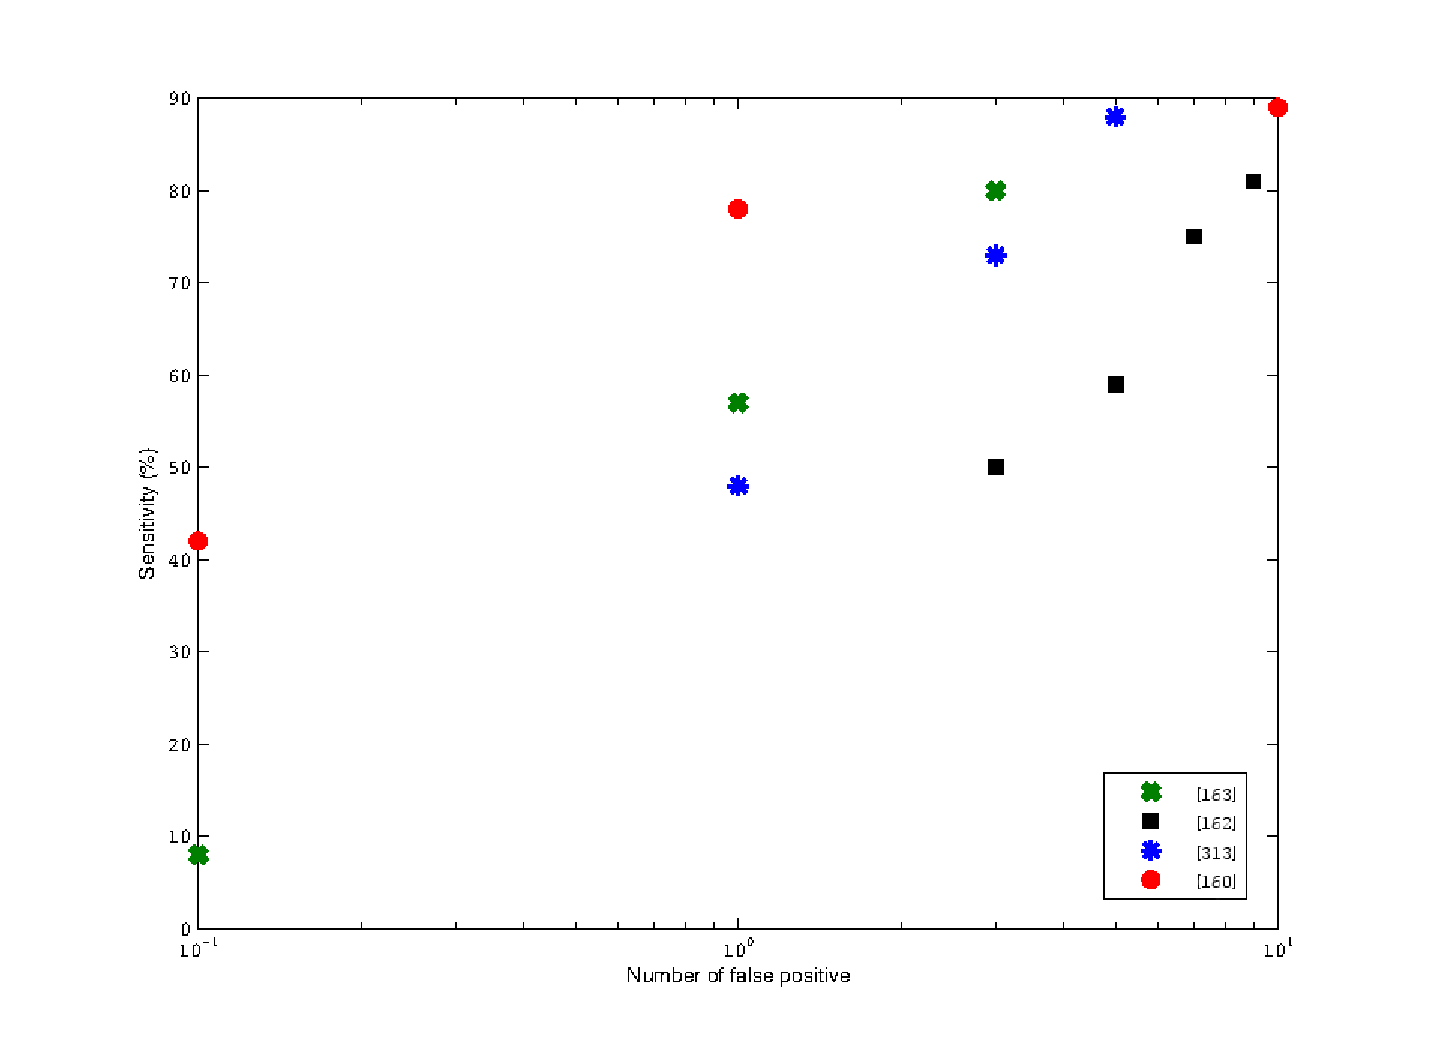
\includegraphics[width=.8\linewidth]{3_review/figures/results/froc.eps}
  \caption{Comparison in terms of \acs*{froc} of the methods using data from \SI{3}{\tesla} \acs*{mri} scanner.}
  \label{fig:froc}
\end{figure}

\begin{figure}
  \centering
 % \hspace{\fill}
  \subfigure[]{
    \label{fig:auc15}
    \begin{tikzpicture}[scale=.7,every node/.style={scale=0.7}]

      \def\labels{
        {\color{blue}\cite{Ampeliotis2008}},
        {\color{blue}\cite{Antic2013}},
        {\color{blue}\cite{Chan2003}},
        {\color{blue}\cite{Giannini2013}},
        {\color{blue}\cite{Langer2009}},
        {\color{blue}\cite{Lopes2011}},
        {\color{blue}\cite{Lv2009}},
        {\color{blue}\cite{Niaf2011}},
        {\color{blue}\cite{Niaf2012}},
        {\color{blue}\cite{Tiwari2009a}},
        {\color{blue}\cite{Tiwari2010}},
        {\color{blue}\cite{Tiwari2012}},
        {\color{blue}\cite{Tiwari2013}},
        {\color{blue}\cite{Vos2008}},
        {\color{blue}\cite{Vos2010}},
        {\color{blue}\cite{lehaire2014computer}},
        {\color{blue}\cite{giannini2015fully}},
        {\color{blue}\cite{Mazzetti2011}},
        {\color{blue}\cite{Puech2009}},
        {\color{blue}\cite{Vos2008a}},
        {\color{blue}\cite{rampun2016computerb}},
        {\color{blue}\cite{rampun2016computer}} 
      }

      \def\reward{90,94,84,87,71,93,97,87,87,84,91,90,85,91,97,75,91,92,77,90,93,93}
      \def\dbSize{25,53,15,10,25,27,55,23,30,15,19,36,29,29,29,35,56,29,100,10,45,45}
      \def\dbClass{1,2,1,1,1,1,2,1,1,1,1,1,1,1,1,1,2,1,3,1,2,2}
      \def\cZoom{3} 
      \def\percentageLabelAngle{90}
      \def\nbeams{22}
      \pgfmathsetmacro\beamAngle{(360/\nbeams)}
      \pgfmathsetmacro\halfAngle{(180/\nbeams)}
      \pgfmathsetmacro\globalRotation{\halfAngle}

      % draw the radiants
      \foreach \n  [count=\ni] in \labels
      {
        \pgfmathsetmacro\cAngle{{(\ni*(360/\nbeams))+\globalRotation}}
        \draw(\cAngle:{\cZoom*1.15})  node[fill=white] {\n};
        \draw [thin] (0,0) -- (\cAngle:{\cZoom*1}) ;

      }

      % draw the % rings 
      \foreach \x in {12.5,25, ...,100} 
      \draw [thin,color=gray!50] (0,0) circle [radius={\cZoom*\x/100}];

      \foreach \x in {50,75,100}
      { 
        \draw [thin,color=black!50] (0,0) circle [radius={\cZoom/100*\x}];
        \foreach \a in {0, 180} \draw ({\percentageLabelAngle+\a}:{\cZoom*0.01*\x}) node  [inner sep=0pt,outer sep=0pt,fill=white,font=\fontsize{8}{8.5}\selectfont]{$\x\%$};
      }

      % draw the path of the percentages
      \def\aux{{\reward}}
      \pgfmathsetmacro\origin{\aux[\nbeams-1]} 
      \draw [semiAuto, thick] (\globalRotation:{\cZoom*\origin/100}) \foreach \n  [count=\ni] in \reward { -- ({(\ni*(360/\nbeams))+\globalRotation}:{\cZoom*\n/100}) } ;

      % label all the percentags
      \foreach \n [count=\ni] in \dbSize 
      {
        \pgfmathsetmacro\cAngle{{(\ni*(360/\nbeams))+\globalRotation}}
        \pgfmathsetmacro\nreward{\aux[\ni-1]}
        \draw (\cAngle:{\cZoom*1.5}) node[align=center] {{\color{semiAuto}\nreward $\%$} \\ {\color{red}\n} };
      } ;

      % draw the database rose
      \def\dbScale{\9}
      \foreach \n [count=\ni] in \dbClass
      \filldraw[fill=red!20!white, draw=red!50!black]
      (0,0) -- ({\ni*(360/\nbeams)-\halfAngle+\globalRotation}:{\cZoom*\n/9}) arc ({\ni*(360/\nbeams)-\halfAngle+\globalRotation}:{\ni*(360/\nbeams)+\halfAngle+\globalRotation}:{\cZoom*\n/9}) -- cycle;
      \foreach \x in {1,2,3}
      \draw [thin,color=red!50!black,dashed] (0,0) circle [radius={\cZoom*\x/9}];

      %% draw the domain of each class 
      \def\puta{17/0/{Multiparametric},
        5/17/{Monoparametric}}

      \foreach \numElm/\contadorQueNoSeCalcular/\name [count=\ni] in \puta
      {

        \pgfmathsetmacro\initialAngle{(\contadorQueNoSeCalcular*\beamAngle)+\halfAngle+\globalRotation}
        \pgfmathsetmacro\finalAngle  {((\numElm+\contadorQueNoSeCalcular)*\beamAngle)+\halfAngle+\globalRotation}
        \pgfmathsetmacro\l  {\cZoom*1.65+.3pt}
        \draw (\initialAngle:{\cZoom*1.7}) -- (\initialAngle:{\cZoom*1.1});
        \draw [ |<->|,>=latex] (\initialAngle:\l) arc (\initialAngle:\finalAngle:\l) ;     
        \pgfmathsetmacro\r  {\cZoom*1.65+.45pt}
        {\draw [decoration={raise=4pt,text along path,text={\name},text align={center}},decorate] (\finalAngle:\r) arc (\finalAngle:\initialAngle:\r);}
      }
      
    \end{tikzpicture}}\\
  \subfigure[]{
    \label{fig:auc30}
    \begin{tikzpicture}[scale=.7,every node/.style={scale=0.7}]

      \def\labels{
        {\color{blue}\cite{Litjens2014}},
        {\color{blue}\cite{Liu2013}},
        {\color{blue}\cite{Peng2013}},
        {\color{blue}\cite{Viswanath2009}},
        {\color{blue}\cite{Viswanath2011}},
        {\color{blue}\cite{khalvati2015automated}},
        {\color{blue}\cite{Viswanath2012}}
      }

      \def\reward{81,83,95,82,77,90,80}
      \def\dbSize{347,54,48,6,12,20,22}
      \def\dbClass{3,3,2,1,1,1,1}
      \def\cZoom{3} 
      \def\percentageLabelAngle{90}
      \def\nbeams{7}
      \pgfmathsetmacro\beamAngle{(360/\nbeams)}
      \pgfmathsetmacro\halfAngle{(180/\nbeams)}
      \pgfmathsetmacro\globalRotation{\halfAngle}

      % draw the radiants
      \foreach \n  [count=\ni] in \labels
      {
        \pgfmathsetmacro\cAngle{{(\ni*(360/\nbeams))+\globalRotation}}
        \draw(\cAngle:{\cZoom*1.15})  node[fill=white] {\n};
        \draw [thin] (0,0) -- (\cAngle:{\cZoom*1}) ;

      }

      % draw the % rings 
      \foreach \x in {12.5,25, ...,100} 
      \draw [thin,color=gray!50] (0,0) circle [radius={\cZoom*\x/100}];

      \foreach \x in {50,75,100}
      { 
        \draw [thin,color=black!50] (0,0) circle [radius={\cZoom/100*\x}];
        \foreach \a in {0, 180} \draw ({\percentageLabelAngle+\a}:{\cZoom*0.01*\x}) node  [inner sep=0pt,outer sep=0pt,fill=white,font=\fontsize{8}{8.5}\selectfont]{$\x\%$};
      }

      % draw the path of the percentages
      \def\aux{{\reward}}
      \pgfmathsetmacro\origin{\aux[\nbeams-1]} 
      \draw [semiAuto, thick] (\globalRotation:{\cZoom*\origin/100}) \foreach \n  [count=\ni] in \reward { -- ({(\ni*(360/\nbeams))+\globalRotation}:{\cZoom*\n/100}) } ;

      % label all the percentags
      \foreach \n [count=\ni] in \dbSize 
      {
        \pgfmathsetmacro\cAngle{{(\ni*(360/\nbeams))+\globalRotation}}
        \pgfmathsetmacro\nreward{\aux[\ni-1]}
        \draw (\cAngle:{\cZoom*1.5}) node[align=center] {{\color{semiAuto}\nreward $\%$} \\ {\color{red}\n} };
      } ;

      % draw the database rose
      \def\dbScale{\9}
      \foreach \n [count=\ni] in \dbClass
      \filldraw[fill=red!20!white, draw=red!50!black]
      (0,0) -- ({\ni*(360/\nbeams)-\halfAngle+\globalRotation}:{\cZoom*\n/9}) arc ({\ni*(360/\nbeams)-\halfAngle+\globalRotation}:{\ni*(360/\nbeams)+\halfAngle+\globalRotation}:{\cZoom*\n/9}) -- cycle;
      \foreach \x in {1,2,3}
      \draw [thin,color=red!50!black,dashed] (0,0) circle [radius={\cZoom*\x/9}];

      %% draw the domain of each class 
      \def\puta{6/0/{Multiparametric},
        1/6/{Monoparametric}}

      \foreach \numElm/\contadorQueNoSeCalcular/\name [count=\ni] in \puta
      {

        \pgfmathsetmacro\initialAngle{(\contadorQueNoSeCalcular*\beamAngle)+\halfAngle+\globalRotation}
        \pgfmathsetmacro\finalAngle  {((\numElm+\contadorQueNoSeCalcular)*\beamAngle)+\halfAngle+\globalRotation}
        \pgfmathsetmacro\l  {\cZoom*1.65+.3pt}
        \draw (\initialAngle:{\cZoom*1.7}) -- (\initialAngle:{\cZoom*1.1});
        \draw [ |<->|,>=latex] (\initialAngle:\l) arc (\initialAngle:\finalAngle:\l) ;     
        \pgfmathsetmacro\r  {\cZoom*1.65+.45pt}
        {\draw [decoration={raise=4pt,text along path,  text={\name},text align={center}},decorate] (\finalAngle:\r) arc (\finalAngle:\initialAngle:\r);}
      }
      
    \end{tikzpicture}
 }
  %\hspace{\fill}
  \caption[Results comparison from the state-of-the-art in terms of \acs*{auc}.]{Numerical and graphical comparison of the results in terms of \acs*{auc} for \SI{1.5}{\tesla} and \SI{3}{\tesla} \acs*{mri} scanners. The {\color{semiAuto}green} value represents the metric and are graphically reported in the {\color{semiAuto}green} curve in the center of the figure. The {\color{red}red} value and areas correspond to the number of patients in the dataset. The numbers between brackets in {blue\color{blue}} correspond to the reference as reported in \acs{tab}~\ref{tab:sumpap}.}
  \label{fig:auc}
\end{figure}


\begin{figure}%
 \centering
 \hspace*{\fill}
  \subfigure[]{
    \label{fig:sens15}
    \begin{tikzpicture}[scale=.5,every node/.style={scale=0.5}]

      \def\labels{
        {\color{blue}\cite{Artan2009}},
        {\color{blue}\cite{Artan2010}},
        {\color{blue}\cite{Giannini2013}},
        {\color{blue}\cite{Liu2009}},
        {\color{blue}\cite{Lopes2011}},
        {\color{blue}\cite{Ozer2009}},
        {\color{blue}\cite{Ozer2010}},
        {\color{blue}\cite{Tiwari2009a}},
        {\color{blue}\cite{Viswanath2008}},
        {\color{blue}\cite{Mazzetti2011}},
        {\color{blue}\cite{Puech2009}},
        {\color{blue}\cite{Tiwari2008}}
      }

      \def\reward{74,66,79,90,85,76,78,84,88,82,100,87}
      \def\dbSize{10,21,10,11,27,20,20,18,16,10,100,18}
      \def\dbClass{1,2,1,1,2,1,1,1,1,1,3,1}
      \def\cZoom{3} 
      \def\percentageLabelAngle{90}
      \def\nbeams{12}
      \pgfmathsetmacro\beamAngle{(360/\nbeams)}
      \pgfmathsetmacro\halfAngle{(180/\nbeams)}
      \pgfmathsetmacro\globalRotation{\halfAngle}

      % draw the radiants
      \foreach \n  [count=\ni] in \labels
      {
        \pgfmathsetmacro\cAngle{{(\ni*(360/\nbeams))+\globalRotation}}
        \draw(\cAngle:{\cZoom*1.15})  node[fill=white] {\n};
        \draw [thin] (0,0) -- (\cAngle:{\cZoom*1}) ;

      }

      % draw the % rings 
      \foreach \x in {12.5,25, ...,100} 
      \draw [thin,color=gray!50] (0,0) circle [radius={\cZoom*\x/100}];

      \foreach \x in {50,75,100}
      { 
        \draw [thin,color=black!50] (0,0) circle [radius={\cZoom/100*\x}];
        \foreach \a in {0, 180} \draw ({\percentageLabelAngle+\a}:{\cZoom*0.01*\x}) node  [inner sep=0pt,outer sep=0pt,fill=white,font=\fontsize{8}{8.5}\selectfont]{$\x\%$};
      }

      % draw the path of the percentages
      \def\aux{{\reward}}
      \pgfmathsetmacro\origin{\aux[\nbeams-1]} 
      \draw [semiAuto, thick] (\globalRotation:{\cZoom*\origin/100}) \foreach \n  [count=\ni] in \reward { -- ({(\ni*(360/\nbeams))+\globalRotation}:{\cZoom*\n/100}) } ;

      % label all the percentags
      \foreach \n [count=\ni] in \dbSize 
      {
        \pgfmathsetmacro\cAngle{{(\ni*(360/\nbeams))+\globalRotation}}
        \pgfmathsetmacro\nreward{\aux[\ni-1]}
        \draw (\cAngle:{\cZoom*1.5}) node[align=center] {{\color{semiAuto}\nreward $\%$} \\ {\color{red}\n} };
      } ;

      % draw the database rose
      \def\dbScale{\9}
      \foreach \n [count=\ni] in \dbClass
      \filldraw[fill=red!20!white, draw=red!50!black]
      (0,0) -- ({\ni*(360/\nbeams)-\halfAngle+\globalRotation}:{\cZoom*\n/9}) arc ({\ni*(360/\nbeams)-\halfAngle+\globalRotation}:{\ni*(360/\nbeams)+\halfAngle+\globalRotation}:{\cZoom*\n/9}) -- cycle;
      \foreach \x in {1,2,3}
      \draw [thin,color=red!50!black,dashed] (0,0) circle [radius={\cZoom*\x/9}];

      %% draw the domain of each class 
      \def\puta{9/0/{Multiparametric},
        3/9/{Monoparametric}}

      \foreach \numElm/\contadorQueNoSeCalcular/\name [count=\ni] in \puta
      {

        \pgfmathsetmacro\initialAngle{(\contadorQueNoSeCalcular*\beamAngle)+\halfAngle+\globalRotation}
        \pgfmathsetmacro\finalAngle  {((\numElm+\contadorQueNoSeCalcular)*\beamAngle)+\halfAngle+\globalRotation}
        \pgfmathsetmacro\l  {\cZoom*1.65+.3pt}
        \draw (\initialAngle:{\cZoom*1.7}) -- (\initialAngle:{\cZoom*1.1});
        \draw [ |<->|,>=latex] (\initialAngle:\l) arc (\initialAngle:\finalAngle:\l) ;     
        \pgfmathsetmacro\r  {\cZoom*1.65+.45pt}
        {\draw [decoration={raise=4pt,text along path,  text={\name},text align={center}},decorate] (\finalAngle:\r) arc (\finalAngle:\initialAngle:\r);}
      }
      
    \end{tikzpicture}
}\hfill
  \subfigure[]{
    \label{fig:spec15}
    \begin{tikzpicture}[scale=.5,every node/.style={scale=0.5}]

      \def\labels{
        {\color{blue}\cite{Artan2009}},
        {\color{blue}\cite{Artan2010}},
        {\color{blue}\cite{Giannini2013}},
        {\color{blue}\cite{Liu2009}},
        {\color{blue}\cite{Lopes2011}},
        {\color{blue}\cite{Ozer2009}},
        {\color{blue}\cite{Ozer2010}},
        {\color{blue}\cite{Tiwari2009a}},
        {\color{blue}\cite{Viswanath2008}},
        {\color{blue}\cite{Mazzetti2011}},
        {\color{blue}\cite{Puech2009}},
        {\color{blue}\cite{Tiwari2008}}
      }

      \def\reward{82,72,84,88,93,75,74,81,85,82,43,85}
      \def\dbSize{10,21,10,11,27,20,20,18,16,10,100,18}
      \def\dbClass{1,2,1,1,2,1,1,1,1,1,3,1}
      \def\cZoom{3} 
      \def\percentageLabelAngle{90}
      \def\nbeams{12}
      \pgfmathsetmacro\beamAngle{(360/\nbeams)}
      \pgfmathsetmacro\halfAngle{(180/\nbeams)}
      \pgfmathsetmacro\globalRotation{\halfAngle}

      % draw the radiants
      \foreach \n  [count=\ni] in \labels
      {
        \pgfmathsetmacro\cAngle{{(\ni*(360/\nbeams))+\globalRotation}}
        \draw(\cAngle:{\cZoom*1.15})  node[fill=white] {\n};
        \draw [thin] (0,0) -- (\cAngle:{\cZoom*1}) ;

      }

      % draw the % rings 
      \foreach \x in {12.5,25, ...,100} 
      \draw [thin,color=gray!50] (0,0) circle [radius={\cZoom*\x/100}];

      \foreach \x in {50,75,100}
      { 
        \draw [thin,color=black!50] (0,0) circle [radius={\cZoom/100*\x}];
        \foreach \a in {0, 180} \draw ({\percentageLabelAngle+\a}:{\cZoom*0.01*\x}) node  [inner sep=0pt,outer sep=0pt,fill=white,font=\fontsize{8}{8.5}\selectfont]{$\x\%$};
      }

      % draw the path of the percentages
      \def\aux{{\reward}}
      \pgfmathsetmacro\origin{\aux[\nbeams-1]} 
      \draw [semiAuto, thick] (\globalRotation:{\cZoom*\origin/100}) \foreach \n  [count=\ni] in \reward { -- ({(\ni*(360/\nbeams))+\globalRotation}:{\cZoom*\n/100}) } ;

      % label all the percentags
      \foreach \n [count=\ni] in \dbSize 
      {
        \pgfmathsetmacro\cAngle{{(\ni*(360/\nbeams))+\globalRotation}}
        \pgfmathsetmacro\nreward{\aux[\ni-1]}
        \draw (\cAngle:{\cZoom*1.5}) node[align=center] {{\color{semiAuto}\nreward $\%$} \\ {\color{red}\n} };
      } ;

      % draw the database rose
      \def\dbScale{\9}
      \foreach \n [count=\ni] in \dbClass
      \filldraw[fill=red!20!white, draw=red!50!black]
      (0,0) -- ({\ni*(360/\nbeams)-\halfAngle+\globalRotation}:{\cZoom*\n/9}) arc ({\ni*(360/\nbeams)-\halfAngle+\globalRotation}:{\ni*(360/\nbeams)+\halfAngle+\globalRotation}:{\cZoom*\n/9}) -- cycle;
      \foreach \x in {1,2,3}
      \draw [thin,color=red!50!black,dashed] (0,0) circle [radius={\cZoom*\x/9}];

      %% draw the domain of each class 
      \def\puta{9/0/{Multiparametric},
        3/9/{Monoparametric}}

      \foreach \numElm/\contadorQueNoSeCalcular/\name [count=\ni] in \puta
      {

        \pgfmathsetmacro\initialAngle{(\contadorQueNoSeCalcular*\beamAngle)+\halfAngle+\globalRotation}
        \pgfmathsetmacro\finalAngle  {((\numElm+\contadorQueNoSeCalcular)*\beamAngle)+\halfAngle+\globalRotation}
        \pgfmathsetmacro\l  {\cZoom*1.65+.3pt}
        \draw (\initialAngle:{\cZoom*1.7}) -- (\initialAngle:{\cZoom*1.1});
        \draw [ |<->|,>=latex] (\initialAngle:\l) arc (\initialAngle:\finalAngle:\l) ;     
        \pgfmathsetmacro\r  {\cZoom*1.65+.45pt}
        {\draw [decoration={raise=4pt,text along path,  text={\name},text align={center}},decorate] (\finalAngle:\r) arc (\finalAngle:\initialAngle:\r);}
      }
      
    \end{tikzpicture}
  }\hspace*{\fill}
  \\
  \hspace*{\fill}
  \subfigure[]{
    \label{fig:sens30}
    \begin{tikzpicture}[scale=.5,every node/.style={scale=0.5}]

      \def\labels{
        {\color{blue}\cite{Peng2013}},
        {\color{blue}\cite{Viswanath2008a}},
        {\color{blue}\cite{trigui2017automatic}},
        {\color{blue}\cite{trigui2016classification}},
        {\color{blue}\cite{cameron2014multiparametric}},
        {\color{blue}\cite{cameron2016maps}},
        {\color{blue}\cite{khalvati2015automated}},
        {\color{blue}\cite{chung2015prostate}},
        {\color{blue}\cite{Matulewicz2013}},
        {\color{blue}\cite{Parfait2012}},
        {\color{blue}\cite{Sung2011}},
        {\color{blue}\cite{samarasinghe2016semi}}
      }

      \def\reward{82,60,91,99,80,86,80,72,63,84,90,92}
      \def\dbSize{48,6,34,34,5,13,20,20,18,22,42,40}
      \def\dbClass{3,1,3,3,1,2,2,2,2,3,3}
      \def\cZoom{3} 
      \def\percentageLabelAngle{90}
      \def\nbeams{12}
      \pgfmathsetmacro\beamAngle{(360/\nbeams)}
      \pgfmathsetmacro\halfAngle{(180/\nbeams)}
      \pgfmathsetmacro\globalRotation{\halfAngle}


      % draw the radiants
      \foreach \n  [count=\ni] in \labels
      {
        \pgfmathsetmacro\cAngle{{(\ni*(360/\nbeams))+\globalRotation}}
        \draw(\cAngle:{\cZoom*1.15})  node[fill=white] {\n};
        \draw [thin] (0,0) -- (\cAngle:{\cZoom*1}) ;

      }

      % draw the % rings 
      \foreach \x in {12.5,25, ...,100} 
      \draw [thin,color=gray!50] (0,0) circle [radius={\cZoom*\x/100}];

      \foreach \x in {50,75,100}
      { 
        \draw [thin,color=black!50] (0,0) circle [radius={\cZoom/100*\x}];
        \foreach \a in {0, 180} \draw ({\percentageLabelAngle+\a}:{\cZoom*0.01*\x}) node  [inner sep=0pt,outer sep=0pt,fill=white,font=\fontsize{8}{8.5}\selectfont]{$\x\%$};
      }

      % draw the path of the percentages
      \def\aux{{\reward}}
      \pgfmathsetmacro\origin{\aux[\nbeams-1]} 
      \draw [semiAuto, thick] (\globalRotation:{\cZoom*\origin/100}) \foreach \n  [count=\ni] in \reward { -- ({(\ni*(360/\nbeams))+\globalRotation}:{\cZoom*\n/100}) } ;

      % label all the percentags
      \foreach \n [count=\ni] in \dbSize 
      {
        \pgfmathsetmacro\cAngle{{(\ni*(360/\nbeams))+\globalRotation}}
        \pgfmathsetmacro\nreward{\aux[\ni-1]}
        \draw (\cAngle:{\cZoom*1.5}) node[align=center] {{\color{semiAuto}\nreward $\%$} \\ {\color{red}\n} };
      } ;

      % draw the database rose
      \def\dbScale{\9}
      \foreach \n [count=\ni] in \dbClass
      \filldraw[fill=red!20!white, draw=red!50!black]
      (0,0) -- ({\ni*(360/\nbeams)-\halfAngle+\globalRotation}:{\cZoom*\n/9}) arc ({\ni*(360/\nbeams)-\halfAngle+\globalRotation}:{\ni*(360/\nbeams)+\halfAngle+\globalRotation}:{\cZoom*\n/9}) -- cycle;
      \foreach \x in {1,2,3}
      \draw [thin,color=red!50!black,dashed] (0,0) circle [radius={\cZoom*\x/9}];

      %% draw the domain of each class 
      \def\puta{8/0/{Multiparametric},
        4/8/{Monoparametric}}

      \foreach \numElm/\contadorQueNoSeCalcular/\name [count=\ni] in \puta
      {

        \pgfmathsetmacro\initialAngle{(\contadorQueNoSeCalcular*\beamAngle)+\halfAngle+\globalRotation}
        \pgfmathsetmacro\finalAngle  {((\numElm+\contadorQueNoSeCalcular)*\beamAngle)+\halfAngle+\globalRotation}
        \pgfmathsetmacro\l  {\cZoom*1.65+.3pt}
        \draw (\initialAngle:{\cZoom*1.7}) -- (\initialAngle:{\cZoom*1.1});
        \draw [ |<->|,>=latex] (\initialAngle:\l) arc (\initialAngle:\finalAngle:\l) ;     
        \pgfmathsetmacro\r  {\cZoom*1.65+.45pt}
        {\draw [decoration={raise=4pt,text along path,  text={\name},text align={center}},decorate] (\finalAngle:\r) arc (\finalAngle:\initialAngle:\r);}
      }
      
    \end{tikzpicture}
}\hfill
  \subfigure[]{
    \label{fig:spec30}
    \begin{tikzpicture}[scale=.5,every node/.style={scale=0.5}]

      \def\labels{
        {\color{blue}\cite{Peng2013}},
        {\color{blue}\cite{Viswanath2008a}},
        {\color{blue}\cite{trigui2017automatic}},
        {\color{blue}\cite{trigui2016classification}},
        {\color{blue}\cite{cameron2014multiparametric}},
        {\color{blue}\cite{cameron2016maps}},
        {\color{blue}\cite{khalvati2015automated}},
        {\color{blue}\cite{chung2015prostate}},
        {\color{blue}\cite{Matulewicz2013}},
        {\color{blue}\cite{Parfait2012}},
        {\color{blue}\cite{Sung2011}},
        {\color{blue}\cite{samarasinghe2016semi}}
      }

      \def\reward{95,66,98,100,70,88,88,92,99,97,77,99}
      \def\dbSize{48,6,34,34,5,13,20,20,18,22,42,40}
      \def\dbClass{3,1,3,3,1,2,2,2,2,3,3}
            
      \def\cZoom{3} 
      \def\percentageLabelAngle{90}
      \def\nbeams{12}
      \pgfmathsetmacro\beamAngle{(360/\nbeams)}
      \pgfmathsetmacro\halfAngle{(180/\nbeams)}
      \pgfmathsetmacro\globalRotation{\halfAngle}

      % draw the radiants
      \foreach \n  [count=\ni] in \labels
      {
        \pgfmathsetmacro\cAngle{{(\ni*(360/\nbeams))+\globalRotation}}
        \draw(\cAngle:{\cZoom*1.15})  node[fill=white] {\n};
        \draw [thin] (0,0) -- (\cAngle:{\cZoom*1}) ;

      }

      % draw the % rings 
      \foreach \x in {12.5,25, ...,100} 
      \draw [thin,color=gray!50] (0,0) circle [radius={\cZoom*\x/100}];

      \foreach \x in {50,75,100}
      { 
        \draw [thin,color=black!50] (0,0) circle [radius={\cZoom/100*\x}];
        \foreach \a in {0, 180} \draw ({\percentageLabelAngle+\a}:{\cZoom*0.01*\x}) node  [inner sep=0pt,outer sep=0pt,fill=white,font=\fontsize{8}{8.5}\selectfont]{$\x\%$};
      }

      % draw the path of the percentages
      \def\aux{{\reward}}
      \pgfmathsetmacro\origin{\aux[\nbeams-1]} 
      \draw [semiAuto, thick] (\globalRotation:{\cZoom*\origin/100}) \foreach \n  [count=\ni] in \reward { -- ({(\ni*(360/\nbeams))+\globalRotation}:{\cZoom*\n/100}) } ;

      % label all the percentags
      \foreach \n [count=\ni] in \dbSize 
      {
        \pgfmathsetmacro\cAngle{{(\ni*(360/\nbeams))+\globalRotation}}
        \pgfmathsetmacro\nreward{\aux[\ni-1]}
        \draw (\cAngle:{\cZoom*1.5}) node[align=center] {{\color{semiAuto}\nreward $\%$} \\ {\color{red}\n} };
      } ;

      % draw the database rose
      \def\dbScale{\9}
      \foreach \n [count=\ni] in \dbClass
      \filldraw[fill=red!20!white, draw=red!50!black]
      (0,0) -- ({\ni*(360/\nbeams)-\halfAngle+\globalRotation}:{\cZoom*\n/9}) arc ({\ni*(360/\nbeams)-\halfAngle+\globalRotation}:{\ni*(360/\nbeams)+\halfAngle+\globalRotation}:{\cZoom*\n/9}) -- cycle;
      \foreach \x in {1,2,3}
      \draw [thin,color=red!50!black,dashed] (0,0) circle [radius={\cZoom*\x/9}];

      %% draw the domain of each class 
      \def\puta{8/0/{Multiparametric},
        4/8/{Monoparametric}}

      \foreach \numElm/\contadorQueNoSeCalcular/\name [count=\ni] in \puta
      {

        \pgfmathsetmacro\initialAngle{(\contadorQueNoSeCalcular*\beamAngle)+\halfAngle+\globalRotation}
        \pgfmathsetmacro\finalAngle  {((\numElm+\contadorQueNoSeCalcular)*\beamAngle)+\halfAngle+\globalRotation}
        \pgfmathsetmacro\l  {\cZoom*1.65+.3pt}
        \draw (\initialAngle:{\cZoom*1.7}) -- (\initialAngle:{\cZoom*1.1});
        \draw [ |<->|,>=latex] (\initialAngle:\l) arc (\initialAngle:\finalAngle:\l) ;     
        \pgfmathsetmacro\r  {\cZoom*1.65+.45pt}
        {\draw [decoration={raise=4pt,text along path,  text={\name},text align={center}},decorate] (\finalAngle:\r) arc (\finalAngle:\initialAngle:\r);}
      }
      
    \end{tikzpicture}
  }
  \hspace*{\fill}
  \caption[Comparison of the state-of-the-art results in terms of \acs*{se} and \acs*{sp}.]{Numerical and graphical comparison of the results in terms of \acs*{se}~\subref{fig:sens15},~\subref{fig:sens30} and \acs*{sp}~\subref{fig:spec15},~\subref{fig:spec30} for \SI{1.5}{\tesla} and \SI{3}{\tesla} \ac{mri} scanners. The value in {\color{semiAuto}green} represents the metric and are graphically reported in the {\color{semiAuto}green} curve in the center of the figure. The {\color{red}red} value and areas correspond to the number of patients in the dataset. The numbers between brackets in {\color{blue}blue} correspond to the reference as reported in \acs{tab}~\ref{tab:sumpap}.}
  \label{fig:sensspec}
\end{figure}


\subsection{Comparison}\label{subsec:chp3:dis:com}

We would like to stress the following findings drawn during the review of the different studies:

\begin{enumerate}
\item Quantitatively, it is difficult to make a fair comparison between the different studies reviewed.
Different factors come into play to elucidate this fact.
Mainly a lack of standardization has to be pointed out in regard to experimental evaluation:
(i) different datasets are used during the evaluation of the frameworks developed hindering an inter-study comparison.
The same conclusion has been recently drawn by~\cite{Litjens2014} supporting this argument;
(ii) the experimental results are not reported with a common metric which leads to the inability to compare the different studies.

\item \label{here} However, multiple studies reported some performance improvements using \ac{mpmri} techniques instead of mono-parametric imaging techniques.
Considering only the most recent studies proposing \ac{cade}-\ac{cadx} frameworks, the following results can be highlighted.
\citeauthor{Viswanath2011} obtained an \ac{auc} of \SI{77}{\percent} using an ensemble learning approach combining the features from the three \ac{mri} modalities --- i.e., \ac{t2w}-\ac{mri}, \ac{dce}--\ac{mri}, and \ac{dw}-\ac{mri}, while the results obtained as standalone modality range from \SIrange{62}{65}{\percent}~\cite{Viswanath2011}. 
\citeauthor{Tiwari2013} drawn similar conclusions by using \ac{t2w}-\ac{mri} and \ac{mrsi} modalities as both in standalone and multi-parametric frameworks with an improved \ac{auc} ranging from \SI{57}{\percent}-\SIrange{76}{85}{\percent}~\cite{Tiwari2013}.
The most recent work of \citeauthor{Litjens2014} obtained an improved \ac{auc} metric from \SI{71}{\percent}-\SI{76}{\percent} considering each modality separately --- i.e., \ac{t2w}-\ac{mri}, \ac{dce}-\ac{mri}, and \ac{dw}-\ac{mri} --- to \SI{89}{\percent} in their \ac{mpmri} framework.

\item The studies comparing particular combination of more than a single modality give rise to the same fact~\cite{Ozer2010,Litjens2011,Liu2013,Litjens2014}: using 3 modalities lead to better performances than using any combination of 2 modalities. 

\item Unlike the previous remark~\ref{here}, no straightforward conclusions can be given regarding the classification performance using each modality in a standalone framework.
The modality being processed by different methods, it does not allow us to conclude if a modality by itself is more suited than another.
However, we are able to distinguish some interesting trends which deserve the attention of the community.
\citeauthor{Tiwari2013} in~\cite{Tiwari2009a,Tiwari2012,Tiwari2013} observed that \ac{mrsi} is a more suitable modality than \ac{t2w} to highlight \ac{cap}.
Moreover, \ac{adc} maps have shown a better discriminative power than \ac{t2w} as well~\cite{Langer2009,Viswanath2011,Peng2013}.
Lately, \citeauthor{Litjens2014} observed that \ac{dw}-\ac{mri} modality is more suitable than both \ac{dce}-\ac{mri} and \ac{t2w}-\ac{mri} to distinguish \ac{cap} in their \ac{cadx} system~\cite{Litjens2014}. 
Recently, \citeauthor{rampun2016computerb} showed, however, some promising results using \ac{t2w}-\ac{mri} only in conjunction with textons and \ac{bow}; this study should be transposed to other \ac{mri} modalities~\cite{rampun2016computerb}.

\item Furthermore, \ac{mpmri} has attracted the attention of both radiologists and computer vision researchers.
Indeed, pioneer research groups included new modalities over years when at the same time, new research groups directly introduced \ac{mpmri} \ac{cad} systems.
These facts lead us to think that \ac{cap} researches will benefit from \ac{mpmri} techniques.

\item When focusing on the different modalities used, it can be pointed out that only \citeauthor{trigui2017automatic} reported the use of all modalities in a single framework by incorporating the \ac{mrsi} modality~\cite{trigui2016classification,trigui2017automatic}.
Although the results reported are promising, the detection has been performed at \ac{mrsi} scale and further investigations need to be carried out.
Nevertheless, \ac{mrsi} has shown some overall good classification performance at the price of a lower resolution as well as an increased acquisition time.
Moreover, \ac{mrsi} analysis is more complex in comparison with the other modalities.
To our mind, \ac{mrsi} could contribute in a \ac{mpmri} framework and should be fused with the other modalities.

\item Lately, 3 studies focused on developing a region-based classification in which \ac{pz} and \ac{cg} will be analyzed separately~\cite{Viswanath2012,Litjens2012,Litjens2014}.
The promising obtained results indicate that this strategy should be further investigated.

\item Recent studies are using quantitative features in addition to \ac{si}.
It seems that these quantitative features provide uncorrelated information with respect to \ac{si} features and should lead to better classification performance when combined all together. 

\item Regarding the methods used in the ``image regularization'' --- i.e., pre-processing, segmentation, and registration --- it is particularly difficult to distinguish the benefit of a method over another since none of the studies focus on making comparison of these processing stages.
The focus is usually entirely based on the ``image classification'' framework where different methods are directly compared.
Note that the performance of a classifier is highly linked with the features vector extracted from particular data.
Hence, one can not conclude that a machine learning method is more appropriate than another, but we can identify a trend in which \ac{svm} as well as ensemble learning classifiers --- i.e., AdaBoost, GentleBoost, and \ac{rf} --- seem to perform better than neural network, \ac{lda}, or Naive Bayes.

\item We would like to draw the attention of the reader on the feature extraction/selection stage.
This processing could reduce the complexity and also allow to find a better feature space for classification.
However, few studies are performing such approaches.
\citeauthor{Niaf2012}, \citeauthor{khalvati2015automated}, \citeauthor{chung2015prostate}, and \citeauthor{rampun2016computer} are successfully applying a scheme to reduce the number of dimensions by selecting the most discriminative features~\cite{Niaf2011,Niaf2012,khalvati2015automated,chung2015prostate,rampun2016computer,rampun2015computer}.
It allows them to obtain improved performances compared with a classification performed with their initial feature vector.
Another group of studies also applied different feature extraction methods~\cite{Viswanath2008a,Viswanath2008,Viswanath2012,Tiwari2007,Tiwari2008,Tiwari2009,Tiwari2010,Tiwari2012,Tiwari2013,lehaire2014computer,rampun2016computerb,rampun2015classifying}.
In these specific cases, no comparison is performed against the original data.
\end{enumerate}

\section{Conclusion}\label{subsec:chp3:dis:gen-dis}

This review leads to some general discussions which could direct to future avenues for research.
As previously mentioned, no open \ac{mpmri} is currently available.
This fact leads to an impossibility to fairly compare the different algorithms designed over years.
Also, the availability of a full \ac{mpmri} dataset, could lead to the development of algorithms which use all the different modalities currently available.
Recalling \acs{tab}~\ref{tab:sumpap}, it can be noted that a single research work provides a solution using at the same time the 4 different modalities.
Also, all the algorithms are focused on one type of scanner only, either \SI{1.5}{\tesla} and \SI{3}{\tesla}.
A dataset including both these types of imaging could allow development of more generic algorithms.

Analyzing the different stages of the \ac{cad} work-flow, it is seen that the current \ac{cad} systems do not include all the pre-processing steps.
It could be interesting to evaluate the improvement using these pre-processing steps on the final results.
Regarding segmentation and registration of the prostate, \ac{cad} systems could greatly benefit from specific research in these areas which could lead to a better automation of those systems.
%Moreover, other segmentation and registration methods does not currently used in \ac{cad} systems could also obtain better results.

% Regarding the classification framework, it seems that the current well-known pattern recognition methods have been widely studied.
% However, more investigations should be carried out regarding the feature detection stage.
% Lately, histogram-based features have shown good capabilities in the field of computer vision and could be further investigated.
% Only one study by~\cite{Liu2013} used some of these features.

Additionally, no research focuses on the problem of imbalanced dataset.
While classifying at the voxel-level, the medical dataset are highly imbalanced regarding the frequencies of \ac{cap} against healthy samples.
Imbalanced data substantially compromises the learning process since most of the standard machine learning algorithms expect balanced class distribution or an equal misclassification cost~\cite{he2009learning}.

%Therefore, after reviewing the state of art, the remaining ... (the state of art is also an objective)
Therefore, it seems important to investigate this field of pattern recognition to improve the classification performance while developing \ac{cad} systems.

%An important point allowing a fair comparison between methods resides in the fact that no common dataset, nor universal evaluation model, nor metric has been defined by the research community allowing such comparison.
% This review aims to have an impact in that respect by providing a novel publicly available multi-parametric and multi-vendor \ac{mri} dataset (from a 1.5 Tesla General Electric scanner and a 3.0 Tesla Siemens scanner).
% This dataset is available at the following website address: \url{http://visor.udg.edu/dataset}. The dataset is composed of the four modalities discussed in this review with their corresponding ground-truth images. For each scanner type, each subset is composed of twenty patients with cancerous lesions and ten healthy patients, having a total of 60 patients. In addition of the repository activity, this website will aim at providing comparison between algorithms developed by the research community.

Therefore, the main objectives of this thesis are to: (i) collect and make available the first \ac{mpmri} dataset; (ii) design, develop, and investigate a \ac{cad} system taking advantage of all available \ac{mri} modalities; (iii) focus on pre-processing methods to improve the classification performance of \ac{cad} systems; (iv) investigate the problem of imbalanced dataset in the \ac{cad} performance; (v) release source code to allow future benchmarking.

